\documentclass[a4paper,12pt,oneside]{bb}
\usepackage{latexsym}
\usepackage{amsmath}
\usepackage{amsfonts}
\usepackage{amsthm}
\usepackage{amssymb}
\usepackage{fncylab}

\usepackage[utf8]{inputenc}

% \usepackage[dvipdfm,
%              pdfstartview={FitH},
%              bookmarks,bookmarksopen,
%              colorlinks,linkcolor={blue},citecolor={red},
%              urlcolor={blue}]{hyperref}

%fonty
\usepackage{charter}
\usepackage{euler}

% tiskove zrcadlo
\topmargin-40pt
\headheight15pt
\headsep10pt
\topskip0pt
\textheight710pt
\oddsidemargin-20pt
\evensidemargin-20pt
\textwidth500pt

\usepackage{graphicx}

%headings
\usepackage{fancyhdr}
\pagestyle{myheadings}
\pagestyle{fancy}

%----------definitions---------------------------
\def\R{\mathbb R}
\def\cl{\text{cl}}
\def\norma#1{\parallel\!#1\!\parallel}
\def\norm#1{\parallel\!#1\!\parallel}

%math definitions
\def\sub{\text{Sub}}
\def\meas{\text{Meas}}
\def\msub{\text{mSub}}
\def\cov{\mbox{\itshape cov}}
\def\non{\mbox{\itshape Non}}
\def\cal{\text{cal}}
\def\msubn{\text{mSub}_{\text{1}}}
\def\subn{\text{Sub}_{\text{1}}}
\def\fn{\text{Fn}}

\def\B{{\mathbb B}}
\def\C{{\mathbb C}}

\def\F{{{\mathcal F}}}
\def\N{{{\mathcal N}}}
\def\E{\mathcal E}

\def\cohen{\mathbf C}

\def\cont{{2^{\aleph_0}}}
\def\force{\Vdash}
\def\aleq{\leq^{*}}
\def\succ{\hbox{succ}}
\def\pw{{{\mathcal P}}}
\def\conc{{^\smallfrown}}
\def\<{\langle}
\def\>{\rangle}
\newcommand{\dl}{\langle\!\langle}
\def\dr{\rangle\!\rangle}


\def\dom{\hbox{dom}}
\def\pomega{\pw(\omega)}
\def\0{\hbox{\bf 0}}
\def\1{\hbox{\bf 1}}
\def\intr#1{%
  \hbox{int}\ #1%
}
\def\cl#1{%
  \hbox{cl}\ #1%
}

\newcommand{\hooklongrightarrow}{\lhook\joinrel\longrightarrow}



%---------numbering of the formulas and theorems---------------
% \newcounter{thm}[section]
% \numberwithin{thm}{section}

%---------numbering of the theorems------------
\swapnumbers

%\renewcommand\subsection{\@startsection{subsection}{2}{\z@}{0pt plus 6pt}{3pt}{\bf}}

%\theoremstyle{plain}
\newtheoremstyle{theorem}% name
  {}%      Space above
  {}%      Space below
  {\itshape}%         Body font
  {}%         Indent amount (empty = no indent, \parindent = para indent)
  {\bfseries\scshape}% Thm head font
  {.}%        Punctuation after thm head
  {.5em}%     Space after thm head: " " = normal interword space;
        %       \newline = linebreak
  {}%         Thm head spec (can be left empty, meaning `normal')
\theoremstyle{theorem}
\newtheorem*{theorem*}{Theorem}
\newtheorem{theorem}[subsection]{Theorem}
\newtheorem{metatheorem}[subsection]{Metatheorem}
\newtheorem{lemma}[subsection]{Lemma}
\newtheorem{proposition}[subsection]{Proposition}
\newtheorem{fact}[subsection]{Fact}
\newtheorem{claim}[subsection]{Claim}
\newtheorem{obs}[subsection]{Observation}
\newtheorem{corollary}[subsection]{Corollary}
\newtheorem{problem}[subsection]{Problem}
%\numberwithin{equation}{section}
\newtheorem{notation}[subsection]{Notation}
%\theoremstyle{remark}
%\newtheorem{remark}[subsection]{Remark}
%\newtheorem*{note}{Note}
\newtheoremstyle{example}% name
  {}%      Space above
  {}%      Space below
  {}%         Body font
  {}%         Indent amount (empty = no indent, \parindent = para indent)
  {\bfseries\scshape}% Thm head font
  {.}%        Punctuation after thm head
  {.5em}%     Space after thm head: " " = normal interword space;
        %       \newline = linebreak
  {}%         Thm head spec (can be left empty, meaning `normal')
\theoremstyle{example}
\newtheorem{example}[subsection]{Example}
\newtheorem{remark}[subsection]{Remark}
\newtheorem*{note}{Note}
%\theoremstyle{definition}
\newtheorem{definition}[subsection]{Definition}

%\labelformat{subsection}{\thechapter.#1}

%vytvoreni indexu
\usepackage{makeidx}
\makeindex

\includeonly{content,prerequisites,orderings,forcing,classical_examples,generic,relations,solovay,work_in_progress}

\usepackage[system=linux]{vpe}
\usepackage[colorlinks,citecolor={blue},bookmarks,bookmarksnumbered]{hyperref}
% \pdfinfo{
%    /Author (B. Balcar, T. Pazák, J. Verner)
%    /Title  (An Exposition of Generic Extensions and Forcing in Set Theory)
%    /Subject (forcing)
%    /Keywords (forcing, set-theory)
% }


%-------------opening--------------------------
\begin{document}
%\tableofcontents
%-------------------------------------------------------------
%-------------------------------------------------------------
%-------------------------------------------------------------
%-------------------------------------------------------------
%---------------------PREREQUISITIES--------------------------
\cfoot{}\rhead{\thepage}
\lhead{{\scshape Content} $\qquad$ {\tiny \today } }

\noindent{\large{\scshape\bfseries %Entre{\' e}
An Exposition of Generic Extensions and Forcing in Set Theory}} \\[0.1cm]

\noindent {\scshape Bohuslav Balcar}, %{\small CTS, J{\' \i}lsk{\' a} 1, Praha 1,
	%Czech Republic, {\ttfamily
	%\href{mailto:balcar@cts.cuni.cz}
	{balcar@math.cas.cz}\footnotemark[1]\footnotetext[1]{Supported in part by
	the GAAV Grant IAA100190509 and by
	the Research Program CTS MSM 0021620845} \\[0.1cm]
\noindent {\scshape Tom{\' a}{\v s} Paz{\' a}k}, %{\small CTS, J{\' \i}lsk{\' a} 1, Praha 1,
	%Czech Republic, {\ttfamily
	%\href{mailto:pazak@cts.cuni.cz}
	{pazak@math.cas.cz}\footnotemark[1] \\[0.1cm]
\noindent {\scshape Jonathan Verner}, %{\small KTIML MFF UK, Praha,
	%Czech Republic {\ttfamily
	%\href{mailto:jonathan.verner@matfyz.cz}
	{jonathan.verner@matfyz.cz}\footnotemark[2]\footnotetext[2]{Supported in part by the GAČR Grant no. 401/09/H007 Logical foundation of semantics}
	\\[0.1cm]
{\tiny \today } \\[0.5cm]

%\maketitle

\thispagestyle{empty}

% \noindent{\Large{\scshape\bfseries Entreé to Generic Extensions and Forcing in Set Theory}} \\[0.1cm]
%
% \noindent {\scshape Bohuslav Balcar}, {\small CTS, J{\' \i}lsk{\' a} 1, Praha 1,
% 	Czech Republic, {\ttfamily balcar@cts.cuni.cz} } \\[0.1cm]
% \noindent {\scshape Jonathan Verner}, {\small KTIML MFF UK, {\ttfamily jonathan.verner@matfyz.cz}\\[0.1cm]
% {\tiny \today } \\[0.5cm]

%\maketitle

%\thispagestyle{empty}

%%%%%%%%%%%%%%%%%%%%%%%%%%%%%%%%%%%%%%%%%%%%%%%%%%%%%%%%%%%%%%%%%%%%%%%%%%%
%%%%%%%%%%%%%%%%%%%%%%%%%%%%%%%%%%%%%%%%%%%%%%%%%%%%%%%%%%%%%%%%%%%%%%%%%%%
\section*{Annotated Content}

\pagenumbering{roman}

${}$\\[-0.1cm] \hrule\hrule
${}$\\[0.2cm]
{\scshape 1. Set Theory Prerequisites \hfill 1 -- 10 } \\[-0.3cm]
\hrule
${}$\\[-0.1cm]

\noindent We mention the axioms of Zermelo~-~Fraenkel Set theory with
axiom of choice (ZFC), transitive sets and ordinal numbers. \ We define
the $V_\alpha$ and $H_\kappa$ hierarchies to illustrate the possibilities of
working with fragments of ZFC. \ We review well-founded relations, induction
and recursion. \ Some basics concerning trees are introduced
together with an example of a well-founded $\omega$-ary tree of rank
$\alpha$, for arbitrary $\alpha < \omega_1$. \ We introduce
the Mostowski collapse and elementary substructure techniques. \ We conclude
the chapter with the definition of a semiset and some motivation for this
concept.

\smallskip

\noindent This chapter is not intended to be self-contained but is rather
meant as a quick summary of what is needed in the sequel.

${}$\\[-0.1cm] \hrule\hrule
${}$\\[0.2cm]
{\scshape 2. Orderings and Boolean Algebras \hfill 11 -- 26 } \\[-0.3cm]
\hrule
${}$\\[-0.1cm]

\noindent In this chapter we introduce many notions that are required to
understand basic forcing combinatorics. We start with the definition of an ordering,
its separative quotient and with some basic combinatorial properties of orderings
e.g. $\kappa$-$cc$, $\kappa$-closed, $\sigma$-centred. These
properties are illustrated on important orderings from forcing
theory such as Cohen's ordering, Collapsing orderings and Levi collapse. \
Rasiowa~-~Sikorski theorem. \ $\Delta$-system lemma. \ We review the
concept of a (M)AD family on $\omega$.

\smallskip

\noindent In the second half we define Boolean algebras and thoroughly investigate
the connection betwixt orderings, Boolean algebras and zero-dimensional
compact Hausdorff spaces. We conclude this chapter with a preparation for
forcing techniques. \ Work with matrices and hierarchy of names. \
Use of elementary submodels.

${}$\\[-0.1cm] \hrule\hrule
${}$\\[0.2cm]
{\scshape 3. Forcing Notion and Generic Filters \hfill 27 -- 33 } \\[-0.3cm]
\hrule
${}$\\[-0.1cm]

First we define when orderings are forcing equivalent and
introduce two criteria. \ We define the generic object and discuss
its existence. \  Some motivation for generic extensions and generic objects
is given. \ We conclude with the Balcar~-~Vopěnka theorem about the canonical
form of a generic object. \ Glimpse of a description of the generic extension.

${}$\\[-0.1cm] \hrule\hrule
${}$\\[0.2cm]
{\scshape 4. Classical Forcing Notions \hfill 34 -- 60 } \\[-0.3cm]
\hrule
${}$\\[-0.1cm]

\noindent We start with a description of basic techniques that will be needed to
introduce classical forcing notions. \ More on working with names, Boolean names,
forcing relation. \ We bring out many phenomena known
from forcing theory together with examples that illustrate these.

\smallskip

\noindent We start with $ccc$ forcings that add new reals. \ Cohen forcing. \
Random forcing, measure algebra. \ We show how to violate CH. \ Proof that $ccc$ forcing
preserves cardinalities and cofinalities. \ Hechler forcing and adding
a dominating real. \ Adding a filter pseudointersection. \ Non $ccc$ forcings.
Mathias forcing, infinite Ramsey theory. \ Three parameter distributivity. \
Base tree techniques.

${}$\\[-0.1cm]
\hrule\hrule
${}$\\[0.2cm]
{\scshape Forcing Relations \hfill 61 -- 70 } \\[-0.3cm]
\hrule
${}$\\[-0.1cm]

\noindent Chapter in progress.

${}$\\[-0.1cm] \hrule\hrule
${}$\\[0.2cm]
{\scshape Generic Extension, Iteration \hfill 70 -- 77 } \\[-0.3cm]
\hrule
${}$\\[-0.1cm]

\noindent Chapter in progress.

${}$\\[-0.1cm] \hrule\hrule
${}$\\[0.2cm]
{\scshape Solovay's Model, Where All Sets are Measurable \hfill 78 -- 102 } \\[-0.3cm]
\hrule
${}$\\[-0.1cm]

\noindent Chapter in progress.

${}$\\[-0.1cm] \hrule\hrule
${}$\\[0.2cm]
{\scshape Index \hfill 103 -- 105 } \\[-0.3cm]
\hrule
${}$\\[-0.1cm]


${}$\\[-0.1cm] \hrule\hrule
${}$\\[0.2cm]
{\scshape References \hfill 106 } \\[-0.3cm]
\hrule
${}$\\[-0.1cm]

\noindent List of references.

%{\tiny \today } \\[0.5cm]

%%%%%%%%%%%%%%%%%%%%%%%%%%%%%%%%%%%%%%%%%%%%%%%%%%%%%%%%%%%%%%%%%%%%%%%
%%%                          END                                    %%%
%%%%%%%%%%%%%%%%%%%%%%%%%%%%%%%%%%%%%%%%%%%%%%%%%%%%%%%%%%%%%%%%%%%%%%%

%-------------------------------------------------------------
%-------------------------------------------------------------
%-------------------------------------------------------------
%-------------------------------------------------------------
%---------------------PREREQUISITIES--------------------------
\cfoot{}\rhead{\thepage}
\lhead{{\scshape Prerequisites} $\qquad$ {\tiny \today } }

% \noindent{\large{\scshape\bfseries %Entre{\' e}
% An Exposition to Generic Extensions and Forcing in Set Theory}} \\[0.1cm]
%
% \noindent {\scshape Bohuslav Balcar}, {\small CTS, J{\' \i}lsk{\' a} 1, Praha 1,
% 	Czech Republic, {\ttfamily
% 	%\href{mailto:balcar@cts.cuni.cz}
% 	{balcar@cts.cuni.cz} } } \\[0.1cm]
% \noindent {\scshape Tom{\' a}{\v s} Paz{\' a}k}, {\small CTS, J{\' \i}lsk{\' a} 1, Praha 1,
% 	Czech Republic, {\ttfamily
% 	%\href{mailto:pazak@cts.cuni.cz}
% 	{pazak@cts.cuni.cz} } } \\[0.1cm]
% \noindent {\scshape Jonathan Verner}, {\small KTIML MFF UK, Praha,
% 	Czech Republic {\ttfamily
% 	%\href{mailto:jonathan.verner@matfyz.cz}
% 	{jonathan.verner@matfyz.cz}} }\\[0.1cm]
% {\tiny \today } \\[0.5cm]

%\maketitle

\thispagestyle{empty}

\pagenumbering{arabic}
%%%%%%%%%%%%%%%%%%%%%%%%%%%%%%%%%%%%%%%%%%%%%%%%%%%%%%%%%%%%
%%%%%%%%%%%%%%%%%%%%%%%%%%%%%%%%%%%%%%%%%%%%%%%%%%%%%%%%%%%%
\section{Set Theory prerequisites}
{\tiny \today } \\[0.5cm]

When we talk about Set Theory we mean the first order predicate theory in a language with equality containing a binary predicate $\in$
with the standard axioms. Formulas describing properties of sets are built up from symbols for variables, predicates ($\in,=$),
logical connectives and quantifiers ($\forall,\exists$). If $\phi(x_0,\ldots,x_n)$ is such a formula, then $\{\langle x_0,\ldots, x_n\rangle:
\phi(x_0,\ldots,x_n)\}$ is the class defined by this formula. E.g. $V=\{x:x=x\}$ is the class of all sets.

\subsection{${}$ \hspace{-1em} Axioms of Zermelo-Fraenkel.}

\begin{itemize}
\item[1.]\emph{Extensionality.} If $x$ and $y$ have the same elements, then
$x=y$ $$(\forall x)(\forall y)((\forall z)(z\in x\leftrightarrow z\in y)\rightarrow x=y)$$
\item[2.]\emph{Pairing.} For any $a$ and $b$ there exists a set $\{a, b\}$ that
contains exactly $a$ and $b$
$$(\forall a)(\forall b)(\exists x)((\forall z)(z\in x\leftrightarrow (z=a\vee z=b)))$$
\item[3.]\emph{Separation (Comprehension).} If $\varphi$ is a formula (with parameter $p$),
then for any set $x$ and $p$ there exists a set $y = \{u \in x : \varphi(u, p)\}$,
i.e. a set that contains all those $u \in x$ that satisfy $\varphi$. Formally, given a formula $\varphi$ with $u$ and $p$ as  free
variables, the formula
$$(\forall p)(\forall x)(\exists y)(\forall u)(u\in y\leftrightarrow y\in x\ \&\ \varphi(u,p))$$
is an axiom of set theory.
\item[4.]\emph{Union.} For any $x$ there exists a set $y =\bigcup x$, the \emph{union}
of all elements of $x$
$$(\forall x)(\exists y)(z\in y\leftrightarrow (\exists u)(u\in x\ \&\ y\in u))$$
\item[5.]\emph{Power Set.} For any $x$ there exists a set $y = \pw (x)$, the
set of all subsets of $x$
$$(\forall x)(\exists y)(\forall z)(z\in y\leftrightarrow (\forall u)(u\in z\rightarrow u\in x))$$
\item[6.]\emph{Infinity.} There exists an infinite set
$$(\exists x)(\emptyset\in x\ \&\ (\forall z)(z\in x\rightarrow z\cup\{z\} \in x))$$
\item[7.]\emph{Replacement.} The image of a set under a (class) mapping is a set. Formally if $\varphi(x,y)$ is a formula then
$$\big[(\forall x)(\forall y)(\forall z)((\varphi(x,y)\ \&\ \varphi(x,z)) \rightarrow z=y)\big]\rightarrow
\big[(\forall a)(\exists b)(y\in b\leftrightarrow (\exists x\in a)\varphi(x,y))\big]$$
 is an axiom.
\item[8.]\emph{Foundation.} Every nonempty set has an $\in$-minimal element
$$(\forall x\neq\emptyset)(\exists y)(y\in x\ \&\ (\forall z)(z\in y\rightarrow z\not\in x))$$
\item[9.]\emph{Choice.} Every set has a choice function
$$(\forall x)(\exists f, \mbox{function})(\forall z)(z\in x\ \&\ z\neq\emptyset\rightarrow f(z)\in z)$$
\end{itemize}

\subsubsection{Comments.}
\begin{itemize}
%  \item[(i)] We introduced only vague formulation of axioms, but each of the
% 	axioms of ZFC can be expressed as a formula, e.g. Foundation can
% 	be stated in following form:
% 	$$
% 	(\forall a \not = \emptyset)\ (\exists x \in a) \ x \cap a = \emptyset.
% 	$$
\item[(i)] In the formal statements of the axiom schemas we tacitly assume that the formulas which serve as
           parameters do not contain ``conflicting free variables''.
\item[(ii)] Some authors include an axiom postulating the existence of a set, i.e. $(\exists x)(x=x)$.
            We do not include it here since it is provable from the axioms of predicate logic with equality.
            Moreover, this is only relevant for fragments which do not include the axiom of infinity.
\item[(iii)] Once we have any set, say $a$, using the third axiom we can prove the existence of the empty set $\{x\in a:x\neq x\}$,
            customarily denoted as $\emptyset$.

 \item[(v)] Formally, our language admits varibles ranging over sets only, however it is
            often useful to talk about collections which are too large to be sets, e.g.
            the universal class $V$. To overcome this difficulty we shall regard formulas
            involving class variables as shorthands. Any formula $\varphi$ naturally determines
            the collection $F=\{x:\varphi(x)\}$ of all sets satisfying $\varphi$. In this
            situation $x\in F$ is a shorthand for $\varphi(x)$. so, e.g. the formula
            $(\forall x\in F)\psi$ is shorthand for $(\forall x)(\varphi\rightarrow\psi)$.
\item[(vi)] The list of axioms is not the shortest possible, e.g. each instance of the axiom of comprehension follows from an instance of the axiom of
            replacement. Also pairing can be proved from the other axioms. However since the list is infinite anyway, this makes \emph{no} difference
            whatsoever.


\end{itemize}


\smallskip

It is customary to let ZF denote Set Theory with axioms 1.--8. and ZFC Set Theory ZF with choice,
i.e. with axiom 9. Occasionally we shall write ZF$^-$ and ZFC$^-$ when we omit axiom 5.

\begin{notation}
Throughout the text we will use the standard notation. For definiteness given a relation $r$
and a class $A$ we let $r[A]=\{y:(\exists a\in A)(\langle a,y\rangle\in r\}$. Similarly for
a function $f$ we let $f[A]=\{y:(\exists a\in A)(f(a)=y)\}$, $f^{-1}[A]=\{x:f(x)\in A\}$.
Moreover the domain of a function (or relation) $f$ will be denoted by $dom(f)$ and the
range of $f$, i.e. $\{y:(\exists x)(f(x)=y)\}$, will be denoted by $rng(f)$.
The corresponding notions for a relation will also be used.
% The ordered pair $\langle x,y\rangle$ will defined according to Kuratowski as $\{\{x\},\{x,y\}\}$ but
% we note that for our purposes any other sensible definition would also do.
\end{notation}

\begin{definition}\label{ts}
{\bf Transitive set.} A set $a$ is \emph{transitive} if every element of $a$
 is a subset of $a$, i.e. $(\forall x\in a)(x\subseteq a)$.
\end{definition}

\begin{fact} Every set $a$ has a \emph{transitive closure}, that is, the smallest transitive
 set containing $a$ as an element. It is denoted by $\mbox{tcl}(a)$.
\end{fact}
\begin{proof} (Hint.) By the axiom of union we can define a (class) function $F$ such that
$F^0(x)=x$, $F(x)=\bigcup x$ and we let $Tcl(a)=\bigcup_{n<\omega} F^n(\{a\})$, i.e.
$\mbox{tcl}(A)=\{A\}\cup A\cup \bigcup A\cup \bigcup\bigcup A\cdots$ is arrived at by iterating
the union operation. See also example \ref{transitive_closure}.
\end{proof}

\begin{definition}\label{ordnumber}{\bf Ordinal number.} A set $\alpha$ is an ordinal number if
 \begin{itemize}
  \item[(i)] $\alpha$ is a transitive set and
  %\item{(ii)}  every element of $\alpha$ is transitive
  \item[(ii)] the $\in$ relation is a linear ordering on $\alpha$, i.e. for all $\beta,\gamma\in\alpha$
               either $\beta\in\gamma$ or $\gamma\in\beta$ or $\beta=\gamma$.
 \end{itemize}
 In other words an ordinal number is the set of all smaller ordinal numbers well-ordered by $\in$.
 The class of all ordinal numbers is denoted by $On$. We write $\alpha<\beta$ to mean $\alpha\in\beta$.
\end{definition}

%The standard definition above is due to John von Neumann.
\begin{definition}[Maximo-lexicographical ordering] The class $On^2$ of pairs of ordinals can be well ordered in a particularly nice way. We say
 that $\langle \alpha_1,\beta_1\rangle\leq_{MLex}\langle\alpha_2,\beta_2\rangle$ iff
 $$
 \max \{\alpha_1,\beta_1\} < \max \{\alpha_2,\beta_2\}\quad \vee\quad \left(\max \{\alpha_1,\beta_1\} = \max \{\alpha_2,\beta_2\}\ \&\
                                                                     \min\{\alpha_1,\beta_1\}<\min\{\alpha_2,\beta_2\}\right)
 $$
 This ordering is a set-like well order, i.e. for each pair $p\in On^2$ the class of pairs which are $\leq_{MLex}$ below $p$ is a set.
\end{definition}


\subsection{${}$ \hspace{-1em} Approximation of the universe.}

% The universal class $V=\{x:x=x\}$ satisfies all axioms of Set Theory, but it is not a set. However there are transitive sets,
% which satisfy a large fragment of the axioms, although not necessarily all of them. The ones most commonly used are
% the two hierarchies of $V_\alpha$'s and $H(\kappa)$'s.

We shall show that there are transitive sets which --- in a sense --- approximate the universe $V$. The ones most commonly used are
the two hierarchies of $V_\alpha$'s and $H(\kappa)$'s.

\begin{definition}{\bf The hierarchy of $V_\alpha$'s.} Using transfinite recursion to iterate the power set operation we define $V_\alpha$
for $\alpha\in On$ as follows:
$$ %\startformula
V_{\emptyset}=\emptyset,\quad V_{\alpha+1}=\pw(V_\alpha),\quad V_\alpha = \bigcup_{\beta<\alpha} V_\beta,\ \mbox{for limit}\ \alpha.
$$ %\stopformula
\end{definition}
\begin{fact} $V=\bigcup\{V_\alpha:\alpha\in On\}$. \\
Note that this fact is equivalent to the axiom of foundation (axiom 8.).
\end{fact}

\begin{definition}\label{rank}{\bf Rank.} To each set $x$ we assign an ordinal number --- its \emph{rank} $\tau(x)$:
 $$ %\startformula
  \tau(x)=min\{\alpha:x\subseteq V_\alpha\}.
 $$ %\stopformula
  It is easily seen that $\tau(x)=sup\{\tau(y)+1:y\in x\}$ for any set $x$.
\end{definition}

\begin{fact}\label{valphaFact} Suppose $\alpha<\beta$ are ordinal numbers. Then
 \begin{itemize}
  \item[(i)] $V_\alpha$ is a transitive set.
  \item[(ii)] $V_\alpha\in V_\beta$.
  \item[(iii)] $On\cap V_\alpha = \alpha$, hence $\alpha\subseteq V_\alpha$ but
	$\alpha\not\in V_\alpha$.
 \end{itemize}
\end{fact}
\begin{proof} (i) Given $x\in V_\alpha$, let $\beta$ be minimal such that $x\in V_\beta$. Clearly $\beta=\gamma+1\leq\alpha$. By the definition of
$V_\beta$ we have that $x\in \mathcal{P(V_\gamma)}$ so $x\subseteq V_\gamma\subseteq V_\beta\subseteq V_\alpha$. (ii) is clear since
$x\in\mathcal{P}(x)$ (iii) We show by induction that $\alpha\subseteq V_\alpha$ and $\alpha\not\in V_\alpha$: this is clear for $\emptyset$. Suppose we
have proven this for all $\beta<\alpha$. If $\alpha$ is limit then by the inductive hypothesis clearly $\alpha\subseteq V_\alpha$ and
easily $\alpha\not\in V_\alpha$. If $\alpha=\beta+1$, then $\alpha=\beta\cup\{\beta\}$ and since $\beta\subseteq V_\beta\subseteq V_\alpha$
by the inductive hypothesis and hence $\beta\in V_\alpha$ by the definition of $V_\alpha$. Similarly $\alpha\not\in V_\alpha$.
\end{proof}

% \begin{definition} Given a set (or class) $M$ and a formula $\varphi$ of set theory, we define the \emph{relativization} $\varphi^M$ of
%  $\varphi$ to $M$ by induction on the complexity of $\varphi$ as follows:
%  \begin{itemize}
%   \item[(i)] If $\varphi$ is atomic, then $\varphi^M$ is $\varphi$,
%   \item[(ii)] if $\varphi$ is of the form $(\forall x)\psi$ then $\varphi^M$ is $(\forall x)(x\in M\rightarrow \psi^M)$ and
%   \item[(iii)] if $\varphi$ is of the form $\neg\psi$ then $\varphi^M$ is $\neg(\psi^M)$.
%  \end{itemize}
%  If $\varphi$ is a closed formula, we say that $M$ satisfies $\varphi$ iff $\varphi^M$ is provable in ZFC. In this case
%  we say that $M$ is a \emph{syntactical model} for $\varphi$.
% \end{definition}

\begin{proposition}\label{valphaApprox}
\begin{itemize}
 \item[]
 \item[(i)] If $\alpha>\omega$ is a limit ordinal number, then $V_\alpha$ satisfies all axioms
 of set theory except for the (full) replacement schema. The class of ordinal numbers in the sense of $V_\alpha$ is
 $\alpha=V_\alpha\cap On$.
 \item[(ii)] $V_\omega$ consists of hereditarily finite sets and
	$(V_\omega,\in)$ is a model of $\mbox{ZF}_{\mbox{fin}} \ $,
	the theory of finite sets. It turns out that it is ``equivalent''
	to the standard model of Peano Arithmetic.
\end{itemize}
\end{proposition}




\begin{definition}\label{H-kappa}{\bf The $H(\kappa)$ hierarchy.} Assume AC. If $\kappa$ is an infinite cardinal number we define
$H(\kappa)$ as follows:
$$ %\startformula
 H(\kappa) = \{x:|\mbox{tcl}(x)|<\kappa\}.
$$ %\stopformula
The set $H(\kappa)$ consists of sets which are hereditarily of cardinality  less then
$\kappa$. The universe $H(\omega_1)$ of hereditarily countable
sets is sometimes denoted by $HC$. Note that $H(\kappa)$ is a set for each $\kappa$.
\end{definition}

In ZFC we again have the following:

\begin{proposition}{\rm (AC)}
 \begin{itemize}
  \item[(i)] Each $H(\kappa)$ is a transitive set.
  \item[(ii)] $V=\bigcup\{H(\kappa):\kappa\ \mbox{is a cardinal number}\}$
 \end{itemize}
\end{proposition}

\begin{definition}\label{strong-limit} Recall, that a cardinal number $\kappa$ is \emph{strongly limit} if
if $2^\lambda<\kappa$ for any $\lambda<\kappa$. An uncountable regular strongly limit cardinal $\kappa$
is called \emph{inaccessible}.
\end{definition}
\begin{proposition}{\rm (AC)} If $\kappa$ is inaccessible or $\kappa=\omega$ then
    $$H(\kappa)=V_\kappa$$
\end{proposition}

Note that the existence of an inaccessible cardinal is not provable in ZFC, however $H(\kappa)=V_\kappa$
for any fixed point of the function $\beth(\kappa)=2^{<\kappa}$.

\begin{proposition}{\rm (AC)}\label{Hkappa2}
\begin{itemize}
 \item[(i)] If $\kappa>\omega$ is a regular cardinal, then $(H(\kappa),\in)$ satisfies all axioms of set theory
 except for the power set axiom 5., i.e. it is a model of $ZFC^-$. (cf. Proposition \ref{valphaApprox}.)
 \item[(ii)] The role of the class of ordinal numbers in the structure $(H(\kappa),\in)$ is played by $\kappa$. %(cf. \in{fact}[valphaFact],iii.)
 \item[(iii)] If a set $b$ is in $H(\kappa)$, then $\pw(b)\subseteq H(\kappa)$.
 \item[(iv)] If $b\in H(\kappa)$ then $\pw(b)\in H(\kappa)$ iff $2^{|b|}<\kappa$.
\end{itemize}
\end{proposition}
\begin{note} Even thought $H(\kappa)$ need not satisfy the full power-set axiom, (iv) tells us that
if we restrict ourselves to sets of ``small'' cardinality --- viz. of cardinality $\lambda$ such that $2^\lambda <\kappa$ ---
the power-set axiom holds.
\end{note}

\subsection{${}$ \hspace{-1em}$H(\kappa)$ as models of fragments of ZFC}
For the purpose of proving
consistency results a model of full ZFC is not needed. More precisely: every proof is a finite
chain (finite in the met\hbox{a-t}heory) of consecutive arguments. Given any finite fragment of ZFC,
there are unboundedly many cardinal numbers $\kappa$ such that $(H(\kappa),\in)$ is a model of
this fragment --- this is the essence of the reflection principle.

Now of course one does not specify the exact fragment of ZFC one needs. The main point
is that it is, at least theoretically, possible to do this. This is the content of the oft
seen phrase

\begin{center}
 ``take sufficiently large $\kappa$''
\end{center}
which in fact means: take $\kappa$ large enough so that $(H(\kappa),\in)$ satisfies
enough axioms to guarantee all the arguments and constructions which we need.

\subsection{${}$ \hspace{-1em}Well-founded relations.}

\begin{definition}\label{ext}
A binary relation $R$ on a set $A$ is \emph{well-founded}
iff each nonempty subset of $A$ contains at least one
 $R$-minimal element, that is for any $\emptyset\neq a\subseteq A$ there is an $x\in a$ with
 $$ %\startformula
  Ext_R(x) \cap a = \emptyset,\quad\hbox{where}\quad Ext_R(x)=\{ y:\langle y,x\rangle\in R\}.
 $$ %\stopformula
\end{definition}

A strict wellordering is an example of a well-founded relation. Well-founded relations
are a generalization of wellorders which are themselves a generalization of the $\in$
relation, viz the axiom of foundation. We shall show (see \ref{WF-recursion}), that recursive
constructions can be carried out along general well-founded relations much in the same way as along $\in$.

\begin{definition}\label{DC}
{\bf Dependent Choice.} The axiom of dependent choice is a weaker
version of the axiom of choice. It says, that
whenever some relation $R$ satisfies
$$ %\startformula
  (\forall x\in dom(R))(\exists y)(yRx)
$$ %\stopformula
then there is an $R$-descending sequence $\langle x_n:n<\omega\rangle$,
i.e. a sequence satisfying $x_{n+1}R x_n$ for each $n<\omega$.
The axiom of dependent choice is abbreviated DC.
\end{definition}

\begin{fact} If we assume DC then a relation $R$ is well-founded iff there are no infinite $R$-decreasing chains.
\end{fact}


% \begin{definition}
% A relation $R$ is \emph{set-like} iff for every set $x$ the class $Ext_R(x)$ is a set.
% \end{definition}

% Well-founded set-like relations are generalizations of the $\in$ relation. The theorems on transfinite induction and recursion can be
% generalized in this setting to induction and recursion over set-like well-founded relations.

% \begin{example}
% \begin{itemize}
%  \item[(i)]  The lexicographical ordering $<_1$ on $On\times On$ is an example of a relation which is well-founded but is not set-like.
%  \item[(ii)] The maximo-lexicographical ordering $<_2$ on $On\times On$ is a well-founded set-like relation:
% %\startformula
% %\startalign[n=3,align={left,middle,left}]
% \begin{align}
% {} & \langle \alpha_1,\beta_1\rangle \leq_2 \langle \alpha_2,\beta_2\rangle & \equiv& \max(\alpha_1,\beta_1) < \max(\alpha_2,\beta_2)\ \hbox{or}\ \\
%                                                                           &&&(\max(\alpha_1,\beta_1) = \max(\alpha_2,\beta_2)\ \&\ %\\ &&&
%                                                                           \min(\alpha_1,\beta_1)< \min(\alpha_2,\beta_2) )
% \end{align}
%  %\stopformula
% \end{itemize}
% \end{example}

\subsection{${}$ \hspace{-1em}Well-founded induction and recursion.}


% \begin{theorem}\label{WF-induction}
% {\rm (Well-founded induction).}
% Suppose $R$ is a well-founded %and set-like
% relation on $A$. Let $X \subset A$ contain the $R$-minimal
% element of $A$ and $X$ satisfies ``the induction
% hypothesis'' $Ext_R(a) \subset X \rightarrow a \in X$. Then
% $X=A$.
% % Furthermore suppose $\phi$ is a formula such that whenever for each $a\in A$ if
% % $(\forall b\in Ext_R(a))\varphi(b) \rightarrow \varphi(a)$. Then $(\forall a\in A)\varphi(a)$.
% \end{theorem}

\begin{theorem}\label{WF-recursion}
{\rm (Well-founded recursion).} Suppose $R$ is a well-founded and set-like
relation on $X$ and $G$ is a mapping defined on $V$.
Then there exists a unique function $F$ defined on $X$ which satisfies
$$ %\startformula
 %F(a) = G(F\upharpoonright Ext_R(a) )\quad\hbox{for each}\ a\in A.
 F(x) = G(\{F(y):y R x \}), \ \mbox{for each}\ x \in X.
$$ %\stopformula
\end{theorem}

% \begin{corollary}
% It follows, as a special case, that there exists a unique function $F_1$ such that
%  $$ %\startformula
%  F_1(a) = G(\{F_1(y):b R a \}).
% $$ %\stopformula
% \end{corollary}

\subsection{${}$ \hspace{-1em}Rank function.}
Every well-founded relation $R$ on $X$ has an associated
\emph{rank function} $\rho_R:X\to On$ which
is defined using well-founded recursion as:
$$ %\startformula
 \rho_R(x)=\hbox{sup}\{\rho_R(y)+1:y R x\},\ \sup \emptyset = 0.
$$ %\stopformula

\smallskip

If $X$ is a set, then the range of $\rho_R$ is an ordinal number and is called the \emph{height} of $R$ on $X$.
If $R$ is a well-ordering, then the height of $R$ is also called the \emph{order type} of $R$.

\smallskip

We shall now introduce the often used concept of a tree and show an application of the rank function on ill-founded trees.


\begin{definition}\label{tree}
{\bf Tree.} A nonempty set $T$ together with a partial order $\leq$ forms a \emph{tree} iff
for each $t\in T$ the set of its predecessors $pred_T(t)=\{s\in T:s< t\}$ is well-ordered by $<$.
\begin{itemize}
 \item[(i)] Similarly to predecessors, we denote $succ_T(t)$ the set of all immediate successors of node $t$ in $T$.
 \item[(ii)] For each $t\in T$ we define the \emph{height} $h_T(t)$ of $t$ as the order type of $(pred_T(t),<)$.
 \item[(iii)] The $\alpha$-th level of $T$, denoted by $T_\alpha$,  is defined as $T_\alpha=\{t\in T:h_T(t)=\alpha\}$.
 \item[(iv)] The height of $T$ is defined to be the rank of $<$ and is equal to $\min\{\alpha:T_\alpha=\emptyset\}$.
 \item[(v)] A maximal linearly ordered subset of $T$ is called a \emph{branch} of $T$. The set of all branches of a tree $T$ will be denoted by $[T]$.
\end{itemize}

\smallskip

By a \emph{subtree} $T' \subset T$ we understand a nonempty subset $T'$ of $T$
which is closed under initial segments, i.e. $(\forall t \in T')$ if $s \leq t$ then $s \in T'$.
\end{definition}


\begin{example}\label{Seq}
Trees of height $\omega$ with a single root, i.e. a smallest element, have a nice representation.
For a set $X$ define $Seq(X)={}^{<\omega}X=\bigcup\{{}^nX:n<\omega\}$,
the set of all finite sequences of
elements of $X$. In case $X=\omega$ we write just $Seq$. A set
$T\subseteq Seq(X)$ closed under initial segments,
i.e. if $f\in T$ and $n\in dom f$ then $f\upharpoonright n\in T$,
is called a tree on $X$. If $X=\kappa$, we say $T$ is a
\emph{$\kappa$-ary tree}, if $X=2$, $T$ is \emph{binary tree}.
If $T$ is a tree on $X$ then  $(T,\subseteq)$ is a tree.

Given a tree $T$ on $X$ we shall identify branches with
elements of ${}^\omega X$ and let $[T]=\{f\in {}^\omega X:(\forall n<\omega)(f\upharpoonright n\in T)\}$
be the set of all branches of $T$.

\end{example}


\begin{definition} A tree is called \emph{well-founded} if the reverse order $>$ is well-founded, otherwise it is \emph{ill-founded}. Beware that we take the
\emph{reverse} order $>$, since $<$ is well-founded by definition!
\end{definition}

\begin{fact}{\rm {(ZF)} }
\begin{itemize}
 \item[(i)] Assume DC. Then a tree is ill-founded iff it has an infinite branch.
 \item[(ii)] Assume DC. A tree of height omega with finite levels must have an infinite branch.
 \item[(iii)] A well-founded binary tree is finite
\end{itemize}


\end{fact}


\begin{example} If $T$ is a well-founded $\omega$-ary tree, then the reverse
inclusion relation on $T$ is
 well-founded, so it has an associated rank function $\rho_T$.
We can then define the rank $r(T)$
 of $T$ to be $\rho_T(\emptyset)$.
\end{example}

\begin{example}{\rm {(DC)} }
If $T$ is a well-founded $\omega$-ary tree, then $r(T)<\omega_1$ and for any $\alpha<\omega_1$
 there is a well-founded $\omega$-ary tree $T^\alpha$ with $r(T^\alpha)=\alpha$.

\medskip

To see that $r(T)<\omega_1$ note that $|T|$ is countable. For the opposite direction
 we proceed by induction.
A tree of rank $1$ is just $\{\emptyset\}$. Suppose $\alpha<\omega_1$ and we have constructed a tree $T^\beta$ of rank $\beta$ for each $\beta<\alpha$.
To construct a tree of rank $\alpha$, take a tree $T$ of height $2$ with $|T_1|=\omega$ and glue the $T^\beta$'s to the branches of $T$ to
get $T^\alpha$.
%
% $we have a tree $T$
% A tree of finite rank is easy to build. A tree of rank $\omega$ is just an infinite union of branches of increasing length.
%
% if $\alpha<\omega_1$, choose for each limit $0<\beta\leq\alpha$ a strictly increasing sequence $\beta_n$
% with $\beta=\bigcup\{\beta_n:n<\omega\}$. We define by induction on $\alpha$ a function $f$ on the full $\omega$-ary tree
% ${}^{<\omega}\omega$ as follows: $f(\emptyset)=\alpha$. If $f(t)=\beta+1$ then $f(t\conc n)=\beta$ for each $n<\omega$.
% If $f(t)=\beta$ and $\beta$ is limit and nonzero, then $f(t\conc n)=\beta_n$. If $f(t)=0$ then $f(t\conc n)=0$.
% Finally we let $T_\alpha=\{t\in{}^{<\omega}\omega:f(t)>0\vee f(t)=0\ \&\ (\forall s\subset t)(f(s)\neq 0)\}$. It
% is easily seen that $r(T_\alpha)=\alpha$ and that $f\upharpoonright T_\alpha$ is the canonical rank function $\rho_{T_\alpha}$.
\end{example}

The following example will be useful in chapter \ref{chapter_generic} when we will compare
transitive models of ZFC.

\begin{example}\label{transitive_closure}
Given a set $A$, let $Tc(A)$ be the set of all $\in$-descending sequences beginning in
A. The set $Tc(A)$ together with inclusion is a tree. By the axiom of foundation
the height of $(Tc(A),\subseteq)$ is at most $\omega$ and the tree has no infinite
branches. For convenience we shall add the empty sequence to $Tc(A)$ so that $Tc(A)$
has a single root.
\end{example}

Given any well-founded tree $T$ we can define the following two functions on $T$:
\begin{eqnarray*}
 f_T(t)  & = &  \{ \ f(t') : \ t' \in \mbox{succ}_T (t) \ \}, \\
 g_T(t)  & = &  \sup\{ \ g(t') + 1 : \ t' \in \mbox{succ}_T (t) \ \}, \
	\mbox{where} \ g(\mbox{leaf}) = 0.
\end{eqnarray*}
and note that $f_T(s)=\emptyset$ if $s$ is a leaf of $T$.

\begin{theorem} The tree $Tc(A)$ codes the set $A$ in the sense that
$f_{Tc(A)}(\emptyset) = \{A\}$. Moreover given any tree $T$ isomorphic to $Tc(A)$,
$f_T(root(T))=\{A\}$, $g_T(root(T)) = g_{Tc(A)}(\emptyset)=rk(A)+1=\min\{\alpha:A\subseteq V_\alpha\}$
and $rng(f_T)=Tcl(\{A\})$.
\end{theorem}


%
% Any set $X$ determines a tree $(Tc(X),\subseteq)$ consisting of
% finite sequences of sets.
% \begin{itemize}
%  \item[(i)] The empty sequence (sequence of length $0$) belongs to
% 	$Tc(X)$.
%  \item[(ii)] The sequence $\langle X \rangle$ of length $1$ belongs to
% 	$Tc(X)$.
%  \item[(iii)] If sequence $\langle X_0,X_1,X_2,\dots, X_n \rangle$ belongs
% 	to $Tc(X)$, then sequence $\langle X_0,X_1,X_2,\dots, X_n, X_{n+1}\rangle$
% 	belongs to $Tc(X)$ provided $X_{n+1} \in X_n$.
% \end{itemize}
% The sequences are ordered by inclusion. By the axiom of foundation,
% the height of $Tc(X)$ is at most $\omega$ and each leaf of the tree
% is an empty set. It is easy to see, that \emph{transitive closure}
% $\mbox{tcl}(X)$ of set $X$ is equal to $\bigcup \{rng(A) : A \in Tc(X)\}$.
%
% \smallskip
%
% Take any tree $(T,\leq)$ isomorphic to $Tc(X)$. Using WF-recursion
% we can define the following functions on $T$.
% \begin{eqnarray*}
%  f(t)  & = &  \{ \ f(t') : \ t' \in \mbox{succ}_T (t) \ \}, \\
%  g(t)  & = &  \sup\{ \ g(t') + 1 : \ t' \in \mbox{succ}_T (t) \ \}, \
% 	\mbox{where} \ g(\mbox{leaf}) = 0.
% \end{eqnarray*}
% Then we have that $f(\mbox{root}) = \{X\}$ and
% $g(\mbox{root}) = \min \{\alpha : x \in V_\alpha \}$.
% \end{example}

% \begin{example}\label{Cantor_Baire}
% Fundamental examples of trees are
% sets of all finite
% sequences of of natural numbers ${}^\omega \omega$ denoted as
% $\mbox{Seq}$
% or finite sequences of $\{0,1\}$ denoted as
% and $\mbox{Seq}(2) = {}^\omega 2$, where the tree ordering is the inclusion.
% $\mbox{Seq}(2)$ is an example of binary tree and
% $\mbox{Seq}$ of $\omega$-ary tree.
% By the definition
% $\mbox{Seq}(2)$ is a subtree of $\mbox{Seq}$.
% The sets of functions ${}^\omega \{0,1\}$ and ${}^\omega \omega$
% can be equipped with natural topology.
%  $$ %\startformula
% d(f,g)=\frac{1}{k+1}, \ \mbox{where} \ k=\min\{n:f(n)\neq g(n)\}.
% $$ %\stopformula
% Then the topological space ${}^\omega \omega$, known as \emph{Baire space} and
% denoted by $\mathcal N$, is homeomorphic to the irrational numbers,
% while ${}^\omega \{0,1\}$ with the very same topology
% is known as \emph{Cantor space}, denoted by $\mathcal C$ and is a compact subspace
% of $\mathcal N$. ${\mathcal N}$ is a classical example of a non-compact Polish space.
% Note that $[Seq] = {}^\omega \omega$ and $[Seq(2)] = {}^\omega \{0,1\}$.
% \end{example}

We now turn to an important theorem that will be useful later on, but first we need a definition.

\begin{definition}
A relation $R$ on a set $A$ is extensional if for $a\neq b\in A$ we have that $Ext_R(a)\neq Ext_R(b)$, where
$Ext_R(a)=\{x\in A: xRa\}$ (see \ref{ext}).
\end{definition}

Note that the axiom of extensionality is equivalent to saying that $\in$ is extensional on $V$.

\begin{theorem}\label{mostowski}
{\scshape (Mostowski collapse).} Suppose $R$ is a well-founded
%, set-like relation on a class
relation on a set $A$.
\begin{itemize}
\item[(i)] There is a transitive set $M$ and a surjective mapping $F:A\to M$ such that $xRy\rightarrow F(x)\in F(y)$.
\item[(ii)] Moreover if $R$ is extensional on $A$, then the mapping $F$ is an isomorphism.
\end{itemize}
\end{theorem}

\begin{proof}
(hint) Using well-founded recursion, define $F(a)=\{F(b):b\in A\ \&\ bRa\}$. To show that $F$ is as required, use well-founded induction.
\end{proof}

% \startlemma Suppose that $M,N$ are transitive models of ZF and one of them satisfies the Axiom of choice.
%  Suppose, moreover, that they have the same subsets of ordinal numbers, i.e. $\pw^M(Ord^M)=\pw^N(Ord^N)$.
%  Then $M=N$.
% \stoplemma
% \begin{proof} Without loss of generality assume $M\models AC$. First we show that $M\subseteq N$. Let $X\in M$ and, since $M\models AC$
% there is bijection $f\in M$ of some ordinal $\delta\in M$ onto the transitive closure of $X$.
% Define a relation $E$ on $\delta$ as follows: $\alpha E\beta\equiv f(\alpha)\in f(\beta)$. Then, by our
% assumption, $E\in N$. Also $E$ is extensional and well-founded in $M$ and, by absoluteness, also in $N$. Applying
% Mostowski collapsing theorem, there is a transitive set $T\in N$ such that $(E,\delta)\equiv (T,\in)$. So also
% $(T,\in)\equiv (Tcl(X),\in)$. But since both $T$ and $Tcl(X)$ are transitive, necessarily $T=Tcl(X)$. So
% $X\in N$.
%
% Now we show $M=N$ by transfinite induction. Assume $X\in N$ and $X\subseteq M$. Find $\alpha\in Ord$ such
% that $X\subseteq V_\alpha^M$ and let $f\in M$ be a bijection from $V_\alpha^M$ into $Ord$. Now since
% $f[X]$ is a set of ordinals and hence $f[X]\in M$ we know that $X=f^{-1}[f[X]]\in M$.
% \end{proof}


\subsection{${}$ \hspace{-1em}Elementary substructures.}

We will focus on countable substructures of the uncountable structures
$(H(\kappa),\in)$ and universal algebras
$A=\langle A,\{f_i:i\in I\}\rangle$. We shall tacitly assume that the set of operations is at most
countable and each of them is finitary. Suppose we have such an algebra $A$.
A nonempty subset $X\subseteq A$ closed under all these operations determines a
subalgebra and whenever $Y\subseteq A$ is infinite, there is an $X\subseteq A$
which is closed under the operations,
contains $Y$ and $|Y|=|X|$. We assume the axiom of choice throughout this section.

\bigskip
Let us first recall the classical definition of a club set on $\omega_1$. The cardinal number
$\omega_1$ ordered by $\in$ carries a natural topology derived from the order. A club on $\omega_1$
is an unbounded subset of $\omega_1$ which is closed in this topology, i.e. is closed under
taking suprema. A standard argument shows that a countable intersection of club sets is again
a club set. A subset of $\omega_1$ is called stationary iff it intersects each club set. The following
is a classical theorem about stationary subsets, which was subsequently generalized by R. Solovay to
higher cardinalities.

\begin{theorem}[Fodor] Any stationary subset of $\omega_1$ can be partitioned into $\omega_1$-many
 disjoint stationary subsets of $\omega_1$.
\end{theorem}

In the context of forcing it turns out that the following generalization of club sets to
different structures is very convenient.

\begin{definition}\label{club}
{\bf Club.} Let $A$ be an infinite set. A family $C\subseteq[A]^{\omega}$ is
\emph{closed unbounded}, or \emph{club}
for short, in $[A]^\omega$ if it is
\begin{itemize}
  \item[(i)] \emph{unbounded,} i.e.
	$(\forall Y\in[A]^\omega)(\exists X\in C)(Y\subseteq X)$ and
  \item[(ii)] \emph{closed,} i.e. for any increasing chain $\{X_n:n<\omega\}$ of elements of
	$C$ the union $\bigcup\{X_n:n<\omega\}$ is again an element of $C$.
\end{itemize}
\end{definition}

\begin{note} In our definition we have only assumed that $A$ is infinite. If it is countable, however, the notion is not very interesting, in particular
the singleton $\{A\}$ is a club.
\end{note}

\begin{note} Observe that if $C$ is a (classical) club on $\omega_1$ then it is also a club in $[\omega_1]^{\omega}$
(more precisely $\{\alpha:\alpha\in C\ \&\ \omega\leq\alpha\}$ is a club in $[\omega_1]^{\omega}$).
\end{note}

\begin{fact}
Suppose $A$ is an infinite set. It is relatively easy to prove that the intersection
of a countable system of clubs in $[A]^{\omega}$ is again
a club in $[A]^{\omega}$. It follows that the system of clubs in $[A]^{\omega}$
generates a $\sigma$-complete filter.
\end{fact}
%
% \begin{fact}{} It is relatively easy to prove the following basic properties. Suppose $A$ is infinite. Then
% \begin{itemize}[i]
% \item[()] The intersection of a countable system of clubs in $[A]^{\omega}$ is a club in $[A]^{\omega}$.
% \item[()] The system of clubs in $[A]^{\omega}$ generates a filter.
% \end{itemize}
% \end{fact}

The following proposition is an algebraic version of the well-known L\"owenheim~-~Skolem theorem from model theory.

 \begin{proposition}\label{algebraic-club-A}
Suppose $A=\langle A,\{f_n:n<\omega\}\rangle$ is an algebra with infinite underlying set $A$.
Then the family of all  countable subalgebras forms a club in $[A]^{\omega}$.
 \end{proposition}

The converse of the proposition also holds (see e.g. \cite{JechST}):

 \begin{proposition}\label{algebraic-club-B}
Suppose that $C$ is a club in $[A]^{\omega}$, then there are operations
$\{f_n:n < \omega\}$ on $A$ such that
 $C$ contains all countable subalgebras of $A$ with given operations.
 \end{proposition}


Having defined closed unbounded families, we can define stationary families.

\begin{definition}\label{stationary}
{\bf Stationary set.} A family $S\subseteq [A]^{\omega}$ is \emph{stationary} if it intersects each club,
i.e. if $C$ is a club in $[A]^{\omega}$, then $S\cap C\neq\emptyset$.
\end{definition}

It follows from propositions \ref{algebraic-club-A}, \ref{algebraic-club-B} that:

% \begin{corollary} A set $S\subseteq [A]^\omega$ is stationary iff for every system $\{f_n:n<\omega\}$ of finitary operations on $A$,
% $S$ contains a set which is closed under these operations.
% \end{corollary}

Consider now the structure $(H(\kappa),\in)$.

\begin{definition}\label{elementary-substructure}
{\bf Elementary substructure.}
Let $X\subseteq H(\kappa)$ be a countable set. We shall say that
$X$ is an \emph{elementary substructure} of $H(\kappa)$, denoted $(X,\in)\preceq (H(\kappa),\in)$, if for each property expressed
by a formula of Set Theory $\varphi(v_1,\ldots,v_n)$ with free variables $v_1,\ldots, v_n$, the following holds:
%\placeformula
$$ %\startformula
(\forall x_1,\ldots,x_n\in X)( (X,\in)\models \varphi[x_1,\ldots,x_n] \equiv (H(\kappa),\in)\models \varphi[x_1,\ldots,x_n] )
$$ %\stopformula
This implies, in particular, that sentences (i.e. closed formulas) of Set Theory are valid in $(X,\in)$ iff they are valid in $(H(\kappa),\in)$.
\end{definition}

\noindent{\bfseries\scshape Relativity principle.}
The concept of an elementary substructure is akin to the Galileo's relativity principle in physics. This principle states that, using physical
experiments, we cannot decide which frame of reference we are in. Similarly, using Set Theoretical properties, we cannot distinguish
whether we are in the elementary substructure or the superstructure. In other words, the validity of statements about elements of $X$
cannot distinguish between $X$ and $H(\kappa)$.


% \begin{note} Note that when deciding the validity of formulas in $X$ the quantifiers range only over $X$ whereas in $H(\kappa)$ they range
% over all of $\kappa$. In particular existential formulas are 'easier to satisfy' in $H(\kappa)$ whereas universal formulas are ``easier to
% satisfy'' in $X$.
% \end{note}

\begin{fact}\label{elementary-fact}
For any $X\preceq H(\kappa)$ the following basic facts are true:
\begin{itemize}
  \item[(i)] $\omega\subseteq X$ since each natural number is definable in $H(\kappa)$ and
  \item[(ii)] $\omega\in X$, since $\omega$ is also definable in $H(\kappa)$,
\end{itemize}
more generally
\begin{itemize}
  \item[(iii)] If $Y\in X$ and $Y$ is countable, then $Y\subseteq X$.
\end{itemize}
\end{fact}

\begin{note}
Countable elementary substructures typically are not transitive sets, and for $\kappa>\omega_1$ are provably not transitive.
             It is hence perfectly possible that some uncountable set is an \emph{element} of the countable substructure. In fact,
             $\omega_1\in X$ whenever $X$ is an elementary substructure of $H(\kappa)$ for $\kappa>\omega_1$.
\end{note}

As with algebras, we have the following often used and important theorem.

\begin{theorem} Suppose $\kappa>\omega$. Then
\begin{itemize}
  \item[(i)] for any countable subset $Y\subseteq H(\kappa)$, there is an
	$X\preceq H(\kappa)$ such that $Y\subseteq X$ and
  \item[(ii)] the set of countable elementary substructures of $H(\kappa)$
	forms a club in $[H(\kappa)]^\omega$.
\end{itemize}
\end{theorem}

Stationary sets on $[A]^\omega$ are important in the theory of proper forcing. For more information on elementary substructures
and their usage e.g. in topology see \cite{DowST}. Here we mention an application in set theory

\begin{theorem} It $\kappa$ is an inaccessible cardinal, then $V_\kappa = H(\kappa)$ and
 $V_\kappa$ is a model of ZFC. Moreover there exists a cardinal number $\lambda<\kappa$
 with countable cofinality such that $V_\lambda$ is a model of ZFC.
\end{theorem}
\begin{proof} By induction find $\alpha_n<\omega$ and elementary substructures $X_n\preceq H(\kappa)$
such that $X_n\subseteq V_{\alpha_n}\subseteq X_{n+1}$. Then $\lambda=\sup\{\alpha_n:n<\omega$ is as required.
\end{proof}


\subsection{${}$ \hspace{-1em} Elementary substructures as proof tools.}
If we want to prove that a given set $a$ has property $\varphi$
the following argument is sometimes useful. We consider a ``sufficiently
large $\kappa$'' such that $a\in H(\kappa)$. Then, taking an elementary
substructure $(X,\in,a)\prec (H(\kappa),\in,a)$, it is sometimes
easier to prove that
$$(X,\in,a) \vDash \varphi (a),$$
By elementarity we get $(H(\kappa),\in,a)\vDash\varphi(a)$ and, since
$\kappa$ was ``sufficiently large'' then also $\mbox{ZFC}\vdash\varphi(a)$.

\subsection{${}$ \hspace{-1em} Interpretations \& finitary consistency proofs.}

We shall now sketch an effective method for proving relative consistency. This
method was used by G\"{o}del to prove the relative consistency with ZF of CH and the
Axiom of choice.

First we introduce the notion of \emph{interpretation} of the language of Set Theory in
Set Theory itself. The language of Set Theory is determined by two basic binary predicates:
equality ($=$) and membership ($\in$). Using these two predicates we may
define, as is customary, further predicates (e.g. $\cup,\emptyset,\omega,\mathbb{R},\ldots$).

To interpret this language in Set Theory, we need to define a class $U$ and two binary relations,
which we shall suggestively call $=^*$ and $\in^*$. We also require that the following basic conditions
are satisfied, i.e. provable in Set Theory,

\begin{itemize}
 \item[(a)] $(\exists x)U$,
 \item[(b)] $\mathcal{=^*}$ is an equivalence relation on $\{x:U(x)\}$ and
 \item[(c)] $(\forall x,y,z)(U(x)\ \&\ U(y)\ \&\ U(z)\rightarrow \big((x\in^*y\ \&\ x=^*z\rightarrow z\in^*y)\ \&\
								      (x\in^*y\ \&\ y=^*z\rightarrow x\in^*z)\big))$.
\end{itemize}

Then we can translate any formula $\varphi$ of Set Theory into the corresponding formula $\varphi^*$ ---
the interpretation of $\varphi$ --- by replacing all occurances of $=$ with $=^*$, $\in$ with $\in^*$ and
$\forall x$ with $(\forall x\in U)$. The precise definition is, of course, by
induction on the complexity of $\varphi$:

\begin{itemize}
 \item[] If $\varphi$ is $x\in y$, then $\varphi^*$ is $x\in^* y$,
 \item[] if $\varphi$ is $x = y$ then $\varphi^*$ is $x=^*y$ and
 \item[] if $\varphi$ is $\neg(\psi)$ then $\varphi^*$ is $\neg(\psi^*)$,
 \item[] if $\varphi$ is $\psi\rightarrow\chi$ then $\varphi^*$ is $\psi^*\rightarrow\chi^*$ and
 \item[] if $\varphi$ is $(\forall x)\psi$ then $\varphi^*$ is $(\forall x)(U\rightarrow\psi^*)$.
\end{itemize}

We shall say that $(U,=^*,\in^*)$ is a \emph{syntactical model} of a theory $T$ if any axiom of
$T$ translates into a provable formula. We say that the model \emph{satisfies} a sentence $\varphi$ if $\varphi^*$
is provable.

\begin{metatheorem} Suppose $(U,=^*,\in^*)$ is a syntactical model of Set Theory which satisfies
some sentence $\varphi$. Then $\varphi$ is consistent with Set Theory.
\end{metatheorem}
\begin{proof} We assume Set Theory is consistent, otherwise the theorem is clear.
Given a sentence $\psi$ provable in Set Theory by induction on the lenght of its proof we
show that it is satisfied by $U,=^*,\in^*$. Now if $\varphi$ were inconsistent,
then $\neg\varphi$ would be provable so also $(\neg\varphi)^*\equiv\neg(\varphi^*)$ would be
provable. Since we assumed $\varphi^*$ is provable we have shown that Set Theory itself is inconsistent
a constradiction.
\end{proof}

A common special case of interpretations is that we only define the class $U$ and let $=^*,\in^*$
be just $=,\in$. In that case the translated formula $\varphi^*$ is often denoted as $\varphi^U$.

\begin{example} If $U\neq\emptyset$ is a transitive class and $\varphi$ is the axiom of extensionality, then
 $\varphi^U$ is provable. Let us call this interpretation transitive. A formula with $\varphi$ with
 free variables $x_0,\ldots,x_n$ is called \emph{absolute} for an interpretation if
 $$
 (\forall x_0,\ldots,x_n\in U)(\varphi^*\leftrightarrow\varphi).
 $$
 Transitive interpretations have the advantage that many formulas are absolute.
 For example $z=\{x,y\}$ is absolute so for any $z\in U$ we have ``(is a pair)$^U$''
 iff $z$ is a pair. This allows us to simplify many arguments in the case of transitive interpretations.
\end{example}

\begin{example}[G\"{o}del] Let $L$ be the class of constructible sets (see e.g. \cite{JechST}).
$L$ is a transitive class.Then if $\varphi$ is an axiom of ZF, then $\varphi^L$ is provable.
Moreover GCH$^L$ and AC$^L$ are provable. It follows that the continuum hypothesis and the
axiom of choice are both consistent with ZF.
\end{example}

\subsection{${}$ \hspace{-1em}Semisets.}
We now introduce a working term which will be used later on.
Please keep in mind that this concept is not generally known in the wide
Set-Theory circles. Nevertheless it is a simple notion and appears to be quite handy for
generic extension. For more details and in-depth discussion of the concept
see \cite{VoHa:72}. For our purposes we shall not assume --- or need --- any
knowledge of this book.

As a motivation for the definition consider the axiom of power set.
Conventionally it is understood to say that the collection of all parts of a set
forms a set. The following interpretation, which leads to the definition of a
semiset, is equally valid: The axiom of powerset says that the collection of
all parts of a set \emph{which are themselves a set} forms a set.

\begin{definition}\label{semiset}
{\bf Semiset.} A \emph{semiset} is a part of a set. A semiset which is not
a set is \emph{proper}.
\end{definition}

Note that each set is a semiset and in our Set Theory there are no proper semisets.
We will now describe two natural scenarios which lead to this notion.


\subsubsection{Motivating semisets.}
{\bf I.} Take an infinite cardinal $\lambda$ and consider $H(\kappa)$ where
$\kappa= (2^\lambda)^+$. We know that
$(H(\kappa),\in)$ is a model of ZFC${}^-$ (see Proposition \ref{Hkappa2}, (i)).
In our special case,
$\pw(\lambda)\in H(\kappa)$ so the power set axiom holds for
$\lambda$. Let $X$ be a countable elementary substructure of $H(\kappa)$
with $\lambda\in X$.

Then $(X,\in)$ is a model for ZFC${}^-$, $\lambda,\pw(\lambda)\in X$ and
$\in$ is a well-founded extensional relation
on $X$. Applying the Mostowski collapse (see Theorem \ref{mostowski})
to obtain a transitive set $M$ and an isomorphism $F$ of $(X,\in)$
and $(M,\in)$. $(M,\in)$ is again a countable model of ZFC${}^-$.
All subsets of $F(\lambda)$ which are not elements
of $M$ are proper semisets from the point of view of $M$.

\medskip
\hskip-\parindent{\bf II.} Another context, where semisets arise, are nonstandard models of ZFC. For example consider the ultrapower $V^\omega/{\mathcal U}$
where ${\mathcal U}$ is a nontrivial ultrafilter on $\omega$. In this structure there are proper semisets which are even parts of a natural number:
the class of standard natural numbers is an example of such a semiset. It has to be proper, since it has no maximal element. Conversely there
are parts of the natural numbers with no minimal elements, so, again, they must be proper semisets.



% \subsubsubject{A last comment}
% The method of forcing invented by P. Cohen is a method which, given suitable proper semisets, allows to extend the universe of sets into a
% new universe where these semisets become regular sets. Moreover the method is flexible in the sense that it allows to control the behavior
% of the new sets. This extension is called the \emph{generic} extension and the method involves the usage of names.

% \subsection{${}$ \hspace{-1em}Questions\ \&\ Answers.}\label{QaA}
%
% ${}$  \medskip

% {\scshape Question.} Why separation is an axiom schema instead of an axiom?
%
% \smallskip
%
% {\scshape Answer.} For each formula $\varphi$, the schema introduces a single axiom. It follows that there are really infinitely many axioms.
% It can be shown, that the theory $ZF$ cannot be finitely acclimatized, i.e. no finite list of axioms is equivalent to $ZF$. However, the collection of axioms is still rather simple, formally speaking, it is recursive. This is important in logic.
%
% \medskip

% {\scshape Question.} What are classes?
%
% \smallskip
%
% {\scshape Answer.} Every formula $\varphi$ of Set Theory naturally determines the collection of all sets satisfying $\varphi$. This collection
% is usually denoted by
% $$ %\startformula
% \{x:\varphi(x)\},
% $$ %\stopformula
% and called a class. We can extend most of the usual set operation to these objects even though, in many cases, e.g. $V=\{x:x=x\}$, $On=\{\alpha:\alpha\ \mbox{is an ordinal}\}$, $E=\{\langle x,y\rangle:x\in y\}$, these objects are {\bf not} sets. Separation axiom implies that the intersection of a class with a set is always a set. Using classes, we can e.g. write $(H(\kappa),E\cap H(\kappa)^2)$ instead of $(H(\kappa),\in)$.
%
% \medskip

% {\scshape Question.} What is the weird symbol $\models$?
%
% \smallskip
%
% {\scshape Answer.} Short answer: satisfaction, a relation between
% relation structures and formalised formulas, well-known from Model Theory.
%
% \medskip
%
% {\scshape Question.} What about the countable model of ZFC?
%
% \smallskip




% \bigskip
%
% For an in-depth discussion of these questions see your local logic guru.

%%%%%%%%%%%%%%%%%%%%%%%%%%%%%%%%%%%%%%%%%%%%%%%%%%%%%%%%%%%%%%%%%%%%%%%
%%%                          END                                    %%%
%%%%%%%%%%%%%%%%%%%%%%%%%%%%%%%%%%%%%%%%%%%%%%%%%%%%%%%%%%%%%%%%%%%%%%%

%-------------------------------------------------------------
%-------------------------------------------------------------
%-------------------------------------------------------------
%-------------------------------------------------------------
%-----------------------ORDERINGS-----------------------------
\cfoot{}\rhead{\thepage}
\lhead{{\scshape Orderings and Boolean Algebras} $\qquad$ {\tiny \today } }

% \noindent{\Large{\scshape\bfseries Entre{\' e} to Generic Extensions and Forcing in Set Theory}} \\[0.1cm]
%
% \noindent {\scshape Bohuslav Balcar}, {\small CTS, J{\' \i}lsk{\' a} 1, Praha 1,
% 	Czech Republic, {\ttfamily \href{mailto:balcar@cts.cuni.cz}{balcar@cts.cuni.cz} } } \\[0.1cm]
% \noindent {\scshape Jonathan Verner}, {\small KTIML MFF UK, {\ttfamily \href{mailto:jonathan.verner@matfyz.cz}{jonathan.verner@matfyz.cz}} }\\[0.1cm]
% {\tiny \today } \\[0.5cm]

%\maketitle

\thispagestyle{empty}

%%%%%%%%%%%%%%%%%%%%%%%%%%%%%%%%%%%%%%%%%%%%%%%%%%%%%%%%%%%%
%%%%%%%%%%%%%%%%%%%%%%%%%%%%%%%%%%%%%%%%%%%%%%%%%%%%%%%%%%%%
\section{Orderings and Boolean algebras}

{\tiny \today } \\[0.5cm]

In this section we shall introduce many notions.
Most of them are elementary and probably already known to the reader.
We will familiarise ourselves with concepts related
to orderings, e.g. dense and predense sets, filters, separative quotients etc.
We shall also mention the important relationship between
an ordered set and a (complete) Boolean algebra. Then we state the
Rasiowa-Sikorski theorem and show an application in
the special case of $\sigma$-complete algebras. The final paragraph will be devoted
to the concept of a Boolean matrix and its use.
The whole section will also be sprinkled with important
examples of orderings.

%
% We shall first talk about the close relationship between partially ordered sets and complete Boolean algebras. Then we shall go on
% to mention their (basic) cardinal characteristics (as e.g. ccc, $\kappa$-cc, height, $\&$ c. We shall also give basic examples of
% partial orders which will later be used as forcing notions for generic extensions. These examples will include the collapsing partial
% order, the order which is used to add many new subsets of the natural numbers (or, equivalently, raise the power of the continuum)
% and the order used to add a new selective (Ramsey) ultrafilter.

\begin{definition}\label{ordering}
{\bf Ordering.}
            An \emph{ordering} (or an \emph{ordered set}) $(P,\leq)$
	    consist of a nonempty set $P$ together with a reflexive and transitive
	    binary relation $\leq$, i.e. $x\leq x$ and $x\leq y\ \&\ y\leq z\rightarrow x\leq y$.
	    If the binary relation is moreover antisymmetric,
            i.e. if $x\leq y\ \&\ y\leq x\rightarrow x=y$, we say that $(P,\leq)$ is a partial order.

            If $x\leq y$ we say that $x$ is smaller than $y$ or that $x$ is below $y$. If $x,y$ are such that for no $z$ both $z\leq x$ and $z\leq y$,
            we say that $x,y$ are \emph{disjoint} or \emph{incompatible} and denote this by $x\perp y$, otherwise they are \emph{compatible}, denoted by $x\parallel y$.
            An element $x$ with no disjoint elements below $x$ is called an \emph{atom}.
\end{definition}

\begin{definition}\label{various} Suppose $P$ is an ordering and $X\subseteq P$.
\begin{itemize}
 \item[(i)] {\bf Antichain.} $X$ is an \emph{antichain} or is called \emph{disjoint} if any
	two distinct elements of $X$ are incompatible. $X$ is a
	\emph{maximal antichain} if it is an antichain and each element of
	$P$ is compatible with some element of $X$.
 \item[(ii)] {\bf Dense.} $X$ is called \emph{predense} if any element of $P$
	is compatible with some element of $X$. $X$ is dense if for any $x\in P$
	there is an element of $X$ which is below $x$.
	$X$ is \emph{predense} (dense) below $x\in P$ if for every element $y$
	of $P$ \emph{below $x$} there is an element $h\in X$ which is
	compatible with (below) $y$.
 \item[(iii)]{\bf Open dense.} $X$ is called \emph{open dense} if it is downward closed and dense,
	i.e. $(\forall p\in P)(\exists q\in X)(q\leq p)$ and $(\forall h\in X)((\leftarrow,h]\subseteq X$, where
	$(\leftarrow,h]=\{p\in P:p\leq x\}$
 \item[(iv)]{\bf Centred.} $X$ is \emph{centred} if for any finite $F\subseteq X$
	there is a $z\in X$ which is below each $x\in F$.
 \item[(v)]{\bf Filter.} $X$ is a \emph{filter} if it is centred and upward closed,
	i.e. $(\forall h\in X)([h,\rightarrow)\subseteq X$
\end{itemize}
\end{definition}

\subsubsection{Comments and facts}

\begin{itemize}
 \item[(a)] Note that some authors prefer to use the term \emph{preorder} or \emph{quasiorder} where we use the term ordering or order.
 \item[(b)] Linear (total) orders (i.e. any two elements are comparable) and orders having the least element cannot contain disjoint elements.
 \item[(c)] A subset $X$ of an ordering $(P,\leq)$ is implicitly ordered by the restriction of $\leq$ to $X$.
%  \item[()]  A $\sigma$-centered ordering is necessarily ccc, but not vice versa.
\end{itemize}

\begin{fact}\label{dense_equivalents} Let $A$ be maximal antichain and $D$ a dense set. Then
 \begin{itemize}
  \item[(i)]  $A$ is a predense set and $\bigcup\{(\leftarrow, a]:a\in A\}$ is an open dense set.
  \item[(ii)]  $A$ has a refinement $B\subseteq D$, that is, $B$ is a maximal antichain and for all
              $b\in B$ there is an $a\in A$ with $b\leq a$.
 \end{itemize}
\end{fact}


\begin{proof} (hint) For $a\in A$ find a maximal antichain $B_a$ in the ordering $((\leftarrow,a]\cap D,\leq)$.
              Then it suffices to take $\bigcup \{B_a:a\in A\}$.
\end{proof}

The following is a first version of the Rasiowa-Sikorski theorem:

\begin{theorem}\label{rasiowa-sikorski}
{\scshape (Rasiowa, Sikorski).} Suppose $\{D_n:n<\omega\}$ is a countable family of dense subsets of an ordering $P$ and $p\in P$.
Then there is a filter $F$ on $P$ such that
$$ %\startformula
p\in F\quad\&\quad (\forall n<\omega)(D_n\cap F\neq\emptyset).
$$ %\stopformula
\end{theorem}
\begin{proof} By induction choose a decreasing sequence $p\geq p_0\geq p_1\cdots\geq p_n\geq\cdots$ such that $p_n\in D_n$. This sequence forms a centred system which
can easily be extended to the required filter $F$.
\end{proof}

%  \subsection{${}$ \hspace{-1em}Basic cardinal characteristics.}
%
%  We shall now introduce the basic cardinal characteristics of ordered sets: cardinality, weight ($\pi$), saturatedness (sat), height ${\mathfrak h}$. For each of these
%  characteristics we define a partition of $P$ into sets which homogeneous with respect to this characteristic.
%
%  The example of cardinality is most instructive: If $p\leq q$ then $|(\leftarrow,p]|\leq|(\leftarrow, q]|$.
%  Since there is no infinite, strictly decreasing sequence of ordinals, we conclude that the set $H=\{p\in P:(\forall q\leq p)(|(\leftarrow,q]|=|(\leftarrow, p]|)\}$
%  is open dense in $P$. Any maximal antichain consisting of $H$ gives rise to a partition of $P$ into sets which are homogeneous in cardinality.
%
%  \begin{definition}\label   Suppose $(P,\leq)$ is a partial order. Then
%   \begin{itemize}
%    \item[()]{(a)} $P$ is $\kappa$-cc if there is no antichain of cardinality $\kappa$ in $P$. If $P$ is $\omega_1$-cc we say it is ccc
%               (satisfies the countable chain condition). The cardinal characteristic sat($P$) is defined to be the minimal $\kappa$ such that $P$ is $\kappa$-cc.
%    \item[()]{(b)} The \emph{weight} of $P$ ($\pi(P)$) is the minimal cardinality of a dense subset of $P$.
%    \item[()]{(c)} Suppose $P$ has no atoms. Then we define the \emph{height} (or \emph{nondistributivity}) of $P$ (${\mathfrak h}(P)$ to be the minimal cardinality of a system
%               ${\mathcal H}$ of dense subsets of $P$ such that the intersection of ${\mathcal H}$ is not dense. If $P$ has atoms, we let ${\mathfrak h}(P)=\infty$.\stopnotation
%   \end{itemize}
%  \end{definition}
%
% \subsubsection{Comments and facts}
% \begin{itemize}
%  \item[()]{(a)} The cardinal characteristic sat$(P)$ is either finite or uncountable.
%  \item[()]{(b)} The cardinal characteristics sat and $\pi$ are both monotone so they have homogeneous partitions (see exercise \in{section}[monotone_cardinal_characteristics]).
%             ${\mathfrak h}$ is not monotone, nevertheless homogeneous partitions for ${\mathfrak h}$ always exist.
%  \item[()]{(c)} The height of $P$ is only interesting for \emph{atomless} (i.e. without atoms) partial orders. Such orders must necessarily be infinite and
%             $\omega\leq{\mathfrak h}(P)\leq|P|$. (Hint: For each $p\in P$ choose $p_0,p_1$ disjoint below p. Extend $\{p_0,p_1\}$ to a maximal antichain $A_p$ in P.
%             Then if \penalty-10000$H_p=\{(\leftarrow\penalty10000,~a]:a\in A_p\}$ and ${\mathcal H}=\{H_p:p\in P\}$ we have that $\bigcap {\mathcal H}=\emptyset$.)
% \end{itemize}

\subsection{${}$ \hspace{-1em}Separative orderings.}

We will see that, from the forcing point of view, the disjointness relation of an ordering plays a crucial role apart from the ordering itself.
\begin{notation}
Suppose $A$ is a subset of $P$. Then we shall write $A^\perp$ to be the set of all elements disjoint with $A$, formally
$A^\perp=\{p\in P:(\forall a\in A)(p\perp a)\}$. In particular $\{x\}^\perp=\{p\in P:x\perp p\}$.
\end{notation}

\begin{definition} An ordering $(P,\leq)$ is called \emph{separative} if for all $x,y\in P$
 $$ %\startformula\pagereference[separation]
    x\not\leq y \rightarrow (\exists z\leq x)(z\perp y). \leqno{(*)}
 $$ %\stopformula
\end{definition}

It is easy to see that (*) can be substituted by any of the following equivalent conditions:
\begin{itemize}
 \item[(i)]  $x\leq y\equiv \{x\}^\perp \supseteq\{y\}^\perp $
 \item[(ii)]  $x\leq y\equiv (\forall z)(z\parallel x\rightarrow z\parallel y)$
 \item[(iii)]  $x\leq y\equiv \{y\}$ is predense below $x$
\end{itemize}
Note that the implications from the left to the right hold in every ordering.

\smallskip

The following definition and fact shows that each ordering can be strengthened to a separative ordering while preserving
the disjointness relation:

\begin{definition}\label{separative-modification}
{\bf Separative modification.} For any ordering $\leq$ on a set $P$ we define its \emph{separative modification}
$\leq_{sp}$ as follows:
$$ %\startformula
 x\leq_{sp} y \equiv \{x\}^\perp \supseteq\{y\}^\perp
$$ %\stopformula
\end{definition}

\begin{fact} Let $(P,\leq)$ be an ordering. Then

 \begin{itemize}
  \item[(i)] $\leq\ \subseteq\ \leq_{sp}$,
  \item[(ii)] $\leq_{sp}$ is a separative ordering of $P$,
  \item[(iii)]  the disjointness relations for $\leq$ and $\leq_{sp}$ coincide.
 \end{itemize}
 Moreover conditions (i-iii) determine the relation $\leq_{sp}$ uniquely.
\end{fact}

From this point of view linear orderings or orderings with a smallest element are not very interesting because
in their separative modification the disjointness relation is trivial (i.e. each two elements are comparable)
and their quotient (see \ref{separative-quotient}) is just the one element partial order.

Every ordering gives rise to a natural equivalence relation and quotient partial order:

 \begin{fact} If $(P,\leq)$ is an ordering we let $x\approx y\equiv x\leq y\ \&\ y\leq x$. Then
 \begin{itemize}
 \item[(i)]  $\approx$ is an equivalence relation and the quotient $(P,\leq)/\hskip-1mm\approx$ is a partial order.
 \item[(ii)]  If $(P,\leq)$ is a separative ordering, then the quotient $(P,\leq)/\hskip-1mm\approx$ is also separative.
 \item[(iii)]  A dense subset of a separative ordering is again a separative ordered set.
\end{itemize}
\end{fact}


\subsection{${}$ \hspace{-1em}Separative quotient.}\label{separative-quotient}
%\begin{notation}\label{separative-quotient}
The equivalence relation from the preceding fact defined from $\leq_{sp}$ is denoted by $\approx_{sp}$. The
quotient partial order $(P,\leq_{sp})/\hskip-1mm\approx_{sp}$ is called the \emph{separative quotient} of $(P,\leq)$.
%\end{notation}

\medskip

The following is trivial

\begin{fact}
$(P,\leq)$ is a separative partial order iff $\approx_{sp}$ is the identity on $P$.
\end{fact}

\begin{fact}
If $(P,\leq)$ is an ordering then
$$ %\startformula
x\approx_{sp}y\equiv(\forall H\subseteq P)(H\ \mbox{is predense below}\ x\ \mbox{iff}\
H\ \mbox{is predense below}\ y).
$$ %\stopformula
\end{fact}


% \begin{fact} If $\B$ and $\C$ are complete Boolean algebras, $H_1\subseteq \B, H_2\subseteq\C$ are dense
%  subsets and $f$ is an order isomorphism of $(H_1,\leq)$ onto $(H_2,\leq)$ then there exists a unique
%  extension $\overline{f}$ of $f$ with domain $\B$ and range $\C$.
% \end{fact}

\subsection{${}$ \hspace{-1em}Examples of orderings.}


The properties of orderings relevant for forcing only depend on the combinatorial properties of dense sets.
The following examples illustrate that there are nonisomorphic orderings with isomorphic dense subsets
(and hence, as will be seen, have isomorphic generic extensions).

First we mention two cardinal characteristics of an ordering:

\begin{definition}
An ordering $P$ is called
 \begin{itemize}
  \item[(i)]{\bf $\kappa$-cc} (or satisfies the {\bf $\kappa$-chain condition}) if any antichain of $P$ has cardinality $<\kappa$. If $\kappa=\omega_1$ we say that $P$ is \emph{ccc}.

  \item[(ii)]{\bf $\kappa$-closed} if for any $\leq$-descending sequence of
	elements of $P$ which is of length $<\kappa$ has a lower bound in $P$.
	If $\kappa=\omega_1$
        we say that $P$ is \emph{$\sigma$-closed}.
 \end{itemize}
\end{definition}

%Note that while the first property is invariant with respect to dense sets, the second one is not.

\subsection{${}$ \hspace{-1em}Countable orderings.}\label{ctble-orderings}

Consider the following three sets of finite functions:
\begin{itemize}\label{defFn}
 \item[(a)]  $Seq = \bigcup\{ ^n\omega:n<\omega\}$,
 \item[(b)]  $Seq_2 = \bigcup\{ ^n2:n<\omega\}$,
 \item[(c)]  $Fn(\omega,2)=\{f;f:D\to\{0,1\},D\in[\omega]^{<\omega}\}$,
\end{itemize}
all ordered by inverse inclusion (i.e. $f\leq g$ iff $f\supseteq g$). These systems are countable separative partial orders without atoms (atomless) with
a largest element which is the empty set.


\begin{proposition}\label{countable-isom-dense}
 Any two countable atomless orderings have isomorphic dense subsets.
\end{proposition}

\begin{proof}
We show that each such order has a countable dense subset $T$ such that $(T,\geq)$ is isomorphic to the full $\omega$-ary tree
$\bigcup\{ ^n\omega : n\in\omega\}$ ordered by inclusion. This clearly suffices. First we enumerate $P=\{p_n:n<\omega\}$ and
for each $p\in P$ we choose an infinite maximal antichain $A_p$ below $p$. To build $T$ proceed by induction on $\omega$ building at step
$n+1$ the $(n+1)$-st level $T_{n+1}$ of $T$ as follows: $T_{n+1}=\bigcup\{A_{p^\prime}:p\in T_n\}$ where $p^\prime\leq p_n, p$ if $p_n$ and
$p$ are compatible, otherwise $p^\prime=p$.
\end{proof}

\subsection{} A natural generalisation of (c) are the two following separative partial orders ($X$ is an infinite set)

\begin{itemize}
 \item[(d)] $Fn(X,\omega)=\{f;f:D\to\omega,D\in[X]^{<\omega}\}$,
 \item[(e)] $Fn(X,\{0,1\})=\{f;f:D\to\{0,1\},D\in[X]^{<\omega}\}$,
\end{itemize}

which again have isomorphic dense subsets:

\begin{proof}
When $|X|=\omega$ see above. Otherwise partition $X$
into countable sets $A_\xi$, $\xi<\kappa$. Using Proposition \ref{countable-isom-dense}
fix $H_\xi, K_\xi$ dense subsets of $F(A_\xi,\omega)$
and $F(A_\xi,2)$ respectively and an isomorphism $\phi_\xi$ of $H_\xi$ onto $K_\xi$.
Now the set $\{f\in F(X,\omega):(\forall\xi<\kappa)(f\upharpoonright A_\xi\in H_\xi)\}$ is dense in $F(X,\omega)$ and
is isomorphic to the corresponding dense set in $F(X,2)$ via the (concatenated) isomorphisms $\phi_\xi$.
\end{proof}

\begin{definition}\label{sigma-centered}
{\bf {$\sigma$-centred.}} An ordering $P$ is \emph{$\sigma$-centred}
if it can be written as a countable union of filters.
\end{definition}

Each $\sigma$-centred ordering is ccc but not vice versa, see below. Also note that each countable ordering is $\sigma$-centred and the
following proposition limits the cardinality from above:

\begin{proposition}
Any $\sigma$-centred separative partial order $P$ is of cardinality at most $\cont$.
\end{proposition}

\begin{proof}
Let $P=\bigcup P_n$ where $P_n$ is a maximal centred family. Then the mapping $\varphi:P\to\pomega$ defined by $\varphi(p)=\{n:p\in P_n\}$ is
one-to-one.
\end{proof}


\begin{proposition}
 Both of the orders defined in (d,e) are ccc.
\end{proposition}


\begin{proof}
We shall only show the ccc property for $F(X,2)$. This is enough, since $F(X,2)$ and $F(X,\omega)$ have isomorphic dense subsets.
In fact we shall show that $F(X,2)$ satisfies an even stronger condition, %(see \in{exercise}[horn_tarski]),
namely we will partition $F(X,2)$ into countably many sets $P_n$ each of which will contain
antichains of size at most $2^n$. This clearly suffices. Put $P_n=\{f\in F(X,2):|\dom f|=n\}$. Take $f_0,\ldots,f_{2^n}\in P_n$.
We show that at least two are compatible. Put $K=\bigcup\{\dom f_i:i\leq2^n\}$. Consider the normalised counting measure $m$ on $\pw( ^K2)$ and let $X_i=\{g;g:K\to2,g\supseteq f_i,|K|<\omega\}$. Then $X_i\cap X_j=\emptyset$ whenever $f_i\perp f_j$. Also $m(X_i)=1/2^n$ and, using the additivity
of measure, we see that at least two of these sets are not disjoint: otherwise $\sum_{i=0}^{2^n} m(X_i) > 1$.
\end{proof}

Moreover both of the orders (d,e) are $\sigma$-centred iff $|X|\leq\cont$.

\subsection{${}$ \hspace{-1em}Countable functions.}
%\mystartpgraf {Countable functions}
%\mystoppgraf

Consider the following two families of (at most) countable functions:
\begin{itemize}
 \item[(f)]  $Fn(\omega_1,\{0,1\},\omega_1)=\{f;f:D\to\{0,1\}:D\in[\omega_1]^{<\omega_1}\}$,
 \item[(g)]  $Fn(\omega_1,{\mathbb R},\omega_1)=\{f;f:D\to{\mathbb R}:D\in[\omega_1]^{<\omega_1}\}$,
\end{itemize}
ordered by reverse inclusion. ${\mathbb R}$ is the real line.
Both of these orders are separative partial orders which are $\sigma$-closed.

\begin{proposition}
The orderings (f) and (g) have isomorphic dense subsets and satisfy $(\cont)^+$-cc. Also below each of their elements there is an antichain
of size $\cont$.
\end{proposition}
\begin{proof} (hint) We show that (g) can be embedded onto a dense subset of (f): choose a partition $\{A_\xi:\xi<\omega_1\}$ of $\omega_1$ into
countable sets and fix a 1-to-1 onto mapping $\phi_\xi:{\mathbb R}\to 2^{A_\xi}$. Then define $\phi:Fn(\omega_1,{\mathbb R},\omega_1)\to Fn(\omega_1,2,\omega_1)$ as follows: $\phi(f)=\bigcup\{ \phi_\xi(f(\xi)):\xi\in\dom f\}$. It is clear that the range of $\phi$ is a dense subset of $Fn(\omega_1,2,\omega_1)$.
\end{proof}

\subsection{${}$ \hspace{-1em}Collapsing ordering.}

Recall that $Seq(\alpha)$ is the set of finite sequences of ordinals $<\alpha$. The \emph{collapsing ordering} is $(Seq(\kappa),\supseteq)$.
It is a separative partial order, mainly interesting only in the case that $\omega<\alpha$. For $\alpha=2,\omega$ it coincides with the orderings
defined in \ref{ctble-orderings}. If $\omega\leq\alpha$ then $Seq(\alpha)$ has cardinality $|\alpha|$ and is $|\alpha|^+$-cc.

We shall see (\ref{macaloon}) that for infinite $\kappa$ the collapsing ordering $Seq(\kappa)$ is `characterised' by the following properties
\begin{itemize}
\item[(i)]  It has cardinality $\kappa$,
\item[(ii)]  it is a countable union of maximal antichains, namely $\{ ^n\kappa:n<\omega\}$,
\item[(iii)]  each element is compatible with $\kappa$-many members of one of the maximal antichains from (ii).
\end{itemize}

\subsection{${}$ \hspace{-1em}Levi collapse.}


The underlying set for the Levi collapse Levi$(\omega,<\!\!\!\kappa)$ consists of finite functions $p$ from $\kappa\times\omega$ into the ordinals
such that $p(\alpha,n)<\alpha$ whenever $(\alpha,n)\in\dom p$. The ordering is by reverse inclusion, i.e. $p\leq q$ iff $p\supseteq q$.

\begin{definition}\label{product}
{\bf Product of orderings.} Suppose $\langle P_i:i\in I\rangle$ are orderings. We define the product ordering.
$$ %\startformula
\prod_{i\in I}P_i=\left\{f: dom\ f\in[I]^{<\omega}, (\forall i\in dom\ f)(f(i)\in P_i)\right\},
$$ %\stopformula
with the ordering defined by
$$ %\startformula
f\leq g\equiv dom\ f\supseteq dom\ g\ \&\ (\forall i\in dom\ g)(f(i)\leq_i g(i))
$$ %\stopformula
\end{definition}

Note that in the literature, it is often assumed that each $P_i$ has a maximal element $\1$ and the product is then defined to be the
subset of the normal Cartesian product where each function has only finitely many values different from $\1$, i.e. has finite support.

\begin{fact}%observation
 $\prod_{\alpha<\kappa} (Seq(\alpha),\supseteq)$ is isomorphic to a dense subset of Levi$(\omega,<\!\!\kappa)$.
\end{fact}%observation

\begin{proposition}\label{levi-isom}
If $\kappa$ is uncountable regular then Levi$(\omega,<\!\!\!\kappa)$
is $\kappa$-cc and below each element there is an antichain of size
$\lambda$ for any $\lambda<\kappa$.
\end{proposition}

Before we prove the proposition we prove the following theorem which is a very useful tool.

\begin{theorem}\label{delta-system-lemma}
{\scshape ({$\Delta$-system lemma}). } Suppose $\kappa>\omega$ is a regular cardinal and $\langle A_\alpha:\alpha<\kappa\rangle$ are finite sets.
Then there exists a \emph{$\Delta$-system} of cardinality $\kappa$, i.e. a set $I\in[\kappa]^\kappa$ and a \emph{kernel} $K$ of the $\Delta$-system such that for each $\alpha,\beta\in I,\alpha\neq\beta$ we have
$A_\alpha\cap A_\beta=K$.

\smallskip

In particular, every uncountable system of finite sets contains an uncountable $\Delta$-system.
\end{theorem}

\begin{proof}
Shrinking if necessary, we can assume each $A_\alpha$ has the same cardinality,
say $n<\omega$. We continue the proof by induction on $n$.
 If $n=1$, then either there is an $x$ such that for $\kappa$-many $\alpha$'s we
have $A_\alpha=\{x\}$ or we can choose $\kappa$-many
distinct $A_\alpha$'s. Assume $n>1$ and the theorem holds for all $k<n$.
Write $A_\alpha=B_\alpha\cup\{x_\alpha\}$. By induction apply the theorem to the system
$\langle B_\alpha:\alpha<\kappa\rangle$ to find $I$.
Then apply the theorem again, this time to $\langle \{x_\alpha\}:\alpha\in I\rangle$ to obtain $I^\prime$. Now
$\langle B_\alpha\cup\{x_\alpha\}:\alpha\in I^\prime\rangle$ is the required $\Delta$-system.
\end{proof}

\begin{proof} {\scshape of Proposition \ref{levi-isom}.}
We use the $\Delta$-system lemma. Suppose for a contradiction that $\{p_\alpha:\alpha<\kappa\}\subseteq L=Levi(\omega,<\!\!\kappa)$ is a disjoint system. Apply the $\Delta$-system
lemma to the domains of the $p_\alpha$'s. We obtain an index set $A\in[\kappa]^\kappa$ and the root $K$ of the delta system. Note that if any two $p,q\in L$ disjoint, then
they are also disjoint when restricted to the intersection of their domains. It follows,
that $\{p_\alpha\upharpoonright K:\alpha\in A\}$ is still a disjoint system, so in particular $p_\alpha\upharpoonright K\neq p_\beta\upharpoonright K$ for any $\alpha,\beta\in A$. But this is a contradiction, since the number of distinct elements in $L$ having domain $K$ is $\leq (\omega\cdot max K)^{<\omega}<\kappa=|A|$.
\end{proof}



% \begin{theorem}Levi$(\omega,<\!\!\kappa)$ has a dense subset isomorphic to
% $$ %\startformula
% \otimes_{\alpha<\kappa}{\mathbb C}_\alpha = \{g\in\prod_{\alpha<\kappa}{\mathbb C}_\alpha:|\{\alpha:g(\alpha)\neq\emptyset\}|<\omega\}.
% $$ %\stopformula
% \end{theorem}


\subsection{${}$ \hspace{-1em}$([\omega]^\omega,\subseteq)$, infinite subsets of $\omega$.}

The important partial ordered set $([\omega]^\omega,\subseteq)$ is an example of an ordering, that is neither separative nor $\sigma$-closed, while the
separative modification \emph{is} $\sigma$-closed. We shall describe the separative modification. For $A,B\in[\omega]^\omega$ it is easy to see that
$$ %\startformula
A\perp B\equiv |A\cap B|<\omega,
$$ %\stopformula
therefore
$$ %\startformula
A\subseteq_{sp} B \equiv |A\setminus B|<\omega\quad\&\quad A \approx_{sp} B\equiv |A \vartriangle  B|<\omega.
$$ %\stopformula

\subsection{${}$ \hspace{-1em}Star notation.}
%\begin{notation}
In this special case, the following \emph{star-notation} is usually employed.
We write $A\subseteq^* B$ and $A=^*B$ instead of
$A\subseteq_{sp} B$ and $A\approx_{sp} B$, respectively.

\smallskip

\noindent A similar `Star' notation is also used in the context of functions in ${}^\omega \omega$, where we write
\begin{eqnarray*}
 f \leq^* g \ & \equiv & \ |\{\ n : f(n) > g(n) \ \}| < \omega, \\
f <^* g \ & \equiv & \ |\{\ n : f(n) \geq g(n) \ \}|< \omega.
\end{eqnarray*}
The ordering $({}^\omega \omega,  \leq *)$ is frequently used and is the object of ongoing research.
%\end{notation}

\begin{fact}
$([\omega]^\omega,\subseteq^*)$ is a $\sigma$-closed separative ordering.
Its separative quotient, after adding a smallest element,
is the quotient Boolean algebra $\pw(\omega)/fin$, where $fin$ is the
ideal of finite subsets of $\omega$.
\end{fact}


\begin{proof}
Suppose $\langle A_n:n<\omega\rangle$ is a $\subseteq^*$-descending sequence.
By induction choose $a_n\in \bigcap_{i<n} A_n\setminus\{a_0,\ldots,a_{n-1}\}$.
Then $\{a_n:n<\omega\}$ is the required lower bound for $\langle A_n:n<\omega\rangle$.
\end{proof}

\begin{definition}\label{mad}
{\bf AD and MAD families.} Antichains and maximal antichains in
$([\omega]^\omega,\subseteq)$ are usually called \emph{almost disjoint (AD)} and
\emph{maximal almost disjoint (MAD)} families on $\omega$ respectively.
\end{definition}

\begin{fact}
\begin{itemize}
\item[(i)]  No MAD family on $\omega$ is countable.
\item[(ii)]  There is an AD family on $\omega$ of size $\cont$.
\end{itemize}
\end{fact}


\begin{proof}
(i) Let $\{A_n:n<\omega\}$ be an AD family. Choose $a_n\in A_n\setminus \bigcup_{i<n} A_n$. Then if $A=\{a_n:n<\omega\}$ we find that $
\{A_n:n<\omega\}\cup\{A\}$ is still an AD family. (ii) We shall construct the AD family on $Seq(2)$ which clearly suffices, since $|Seq(2)|=\omega$.
For each such branch $f\in 2^\omega$, we let $A_f=\{f\upharpoonright n:n<\omega\}\subseteq Seq(2)$ be the branch of $Seq(2)$ corresponding to $f$. Then
$\{A_f:f\in 2^\omega\}$ is the required AD family.
\end{proof}


%\subsection{${}$ \hspace{-1em}Boolean algebras.}

\begin{definition}
{\bf Boolean algebra.}
A \emph{Boolean algebra} $\B=(B,\vee,\wedge,-,\0,\1)$ is a set
$B$ together with the Boolean operations $a\vee b$ (join), $a\wedge b$ (meet), $-a$ (complement)
and two distinguished elements $\0$ and $\1$ satisfying the following:
\begin{itemize}
 \item[(1)]{(commutativity)} $x\wedge y=y\wedge x,\quad x\vee y=y\vee x$
 \item[(2)]{(distributivity)}
	$x\wedge(y\vee z)=(x\wedge y)\vee(x\wedge z),\quad x\vee(y\wedge z)=(x\vee y)\wedge(x\vee z)$
 \item[(3)]{(neutrality)} $x\vee\0=x,\quad x\wedge\1=x$.
 \item[(4)]{(complement)} $x\wedge-x=\0,\quad x\vee-x=\1$.
 \item[(5)]{(nontriviality)} $\0\neq\1$.
\end{itemize}
\end{definition}


%Also note that the associativity of the operations can be
%deduced from the axioms. From the point of view of universal algebra,
Boolean algebras are distributive, complementary lattices.
Note that the axioms of Boolean algebra as presented are dual. Since
different authors use different set of axioms, we sketch a proof
for some of common formulas that are usualy considered as axioms.

\begin{lemma}
 For each $x,y,z$ elements of Boolean algebra the following hold
\begin{itemize}
 \item[(i)] $x \wedge \mathbf 0 = \mathbf 0 \qquad x \vee \mathbf 1 = \mathbf 1$,
 \item[(ii)] {\bfseries absorption}   $x \vee (x \wedge y) = x \qquad x \wedge (x \vee y) = x $,
 \item[(iii)] {\bfseries associativity} $x\wedge (y \wedge z) = (x \wedge y) \wedge z \qquad x \vee (y \vee z) = (x \vee y) \vee z$.
\end{itemize}
\end{lemma}

\begin{proof}
 Equalities in the same row are dual, so it sufices to prove one of them.

\smallskip

\noindent {\itshape (i)} $x \wedge \mathbf{0} = (x \wedge \mathbf{0}) \vee \mathbf{0} =
	(x \wedge \mathbf{0}) \vee (x \wedge -x) = x \wedge (\mathbf{0} \vee -x) = x \wedge -x = \mathbf{0}$.

\smallskip

\noindent {\itshape (ii)} $x = x \wedge \mathbf{1} = x \wedge (\mathbf{1} \vee y) = (x \wedge \mathbf{1}) \vee (x \wedge y)
	= x \vee (x \wedge y)$.

\smallskip

\noindent {\itshape (iii)} To show the associativity we start with the conjuction of both
formulas
$$
\bigl( x \wedge (y \wedge z) \bigr) \vee \bigl( (x \wedge y) \wedge z \bigr) =
	\bigl[ x \vee \bigl( (x \wedge y) \wedge z \bigr) \bigr] \wedge
	\bigl[ (y \wedge z) \vee \bigl( (x \wedge y) \wedge z \bigr) \bigr] = x \wedge \bigl[ y \wedge z \bigr],
$$
since $\bigl[ x \vee \bigl( (x \wedge y) \wedge z \bigr) \bigr] = \bigl( x \vee (x \wedge y) \bigr) \wedge (x \vee z)
= x \wedge (x \vee z) = x$, \\
and $\bigl[ (y \wedge z) \vee \bigl( (x \wedge y) \wedge z \bigr) \bigr] =
\bigl[y \vee \bigl( (x \wedge y) \bigr) \bigr] \wedge z
 = y \wedge z$.
\smallskip

Now we use commutativity to obtain that the same conjuction is equal to $(x \wedge y) \wedge z$
$$
 \bigl( (x \wedge y) \wedge z \bigr) \vee \bigl( x \wedge (y \wedge z) \bigr) =
	\bigl[ (x \wedge y) \vee \bigl( x \wedge ( y \wedge z) \bigr) \bigr] \wedge
	\bigl[ z \vee \bigl( (x \wedge y) \wedge z \bigr) \bigr] = \bigl[ x \wedge y \bigr] \wedge z.
$$
\end{proof}

The canonical ordering on a Boolean algebra is: $a\leq b$ iff $a\wedge b=a$ iff $a\vee b = b$ and hence $\0$ is the smallest element and $\1$ the largest in this ordering.
We let $\B^{+}=B\setminus\{\0\}$. Then $(\B^{+},\leq)$ is a separative partial ordering.

\smallskip

We shall frequently use notions and properties defined for partial orders also
in the context of Boolean algebras. In such cases we always refer to the partial order
$(\B^+,\leq)$. This order is separative, since if $a\not\leq b$
then we can let $c=a-b\neq\0$ and $c\leq a$ while $c\wedge b=\0$, where $a-b=a\wedge(-b)$.

\begin{definition}\label{density}{\bf Density.} The \emph{density} of a Boolean algebra $\pi(B)$ (also called $\pi$-weight) is
 the minimal cardinality of a dense subset of $(B^+,\leq)$.
\end{definition}

\begin{definition}\label{cba}
{\bf Complete Boolean algebra.}
\begin{itemize}
 \item[(i)]  A Boolean algebra is \emph{complete} %(\emph{Dedekind complete})
	if every subset $X\subseteq B$ has an infimum in the canonical ordering,
	denoted by $\bigwedge X$. In this case every subset also has a supremum,
	denoted by $\bigvee X$ and the standard de Morgan laws hold.
	We say that ``$B$ is a cBA'' as a shorthand for ``$B$ is a complete Boolean algebra''.
 \item[(ii)]  A Boolean algebra is \emph{$\sigma$-complete} if every countable subset has a meet (or join).
\end{itemize}
\end{definition}

\begin{definition}\label{generators}
{\bf Generators.} We say that a subset $X\subseteq B^+$ of a complete Boolean algebra $B$
\emph{completely generates} $B$
if there is no proper complete subalgebra of $B$ containing $X$. We define
$$ %\startformula
{\mathfrak g}(B)\ =\ \min \{ |X|:X\subseteq B^+, X\ \mbox{completely generates}\ B^+\}.
$$ %\stopformula
Similarly for a $\sigma$-complete algebra we define a \emph{$\sigma$-completely generating set} and correspondingly ${\mathfrak g}_\omega(B)$, the
smallest cardinality of a set which $\sigma$-completely generates $B$.
\end{definition}


The power-set $\pw(X)$ of a nonempty set $X$ is a typical example of a complete atomic Boolean algebra. The singletons are
atoms and the operation of meet and join correspond to intersection and union respectively with $\0=\emptyset$,
$\1=X$. Subalgebras of this algebra are called \emph{fields} of sets. If they are moreover $\sigma$-subalgebras, then
they are called $\sigma$-fields  of sets.

\begin{example} Given a topological space $(S,\tau)$ there are several natural algebras determined by $(S,\tau)$:
\begin{itemize}
 \item[(i)]  The algebra $Clop(S)$ of closed-and-open, \emph{clopen} for short, subsets of $S$.
 \item[(ii)]  The algebra $Baire(S)$ is the smallest $\sigma$-field which contains all zero sets from S.
             A subset of $S$ is a \emph{zero set} iff it is the preimage of $\{0\}$ under some continuous
             mapping $f:S\to{\mathbb R}$.
 \item[(iii)]  The algebra $Borel(S)$ is the smallest $\sigma$-field which contains all open subsets of $S$.
 \item[(iv)]  The algebra $BP(S)$ consisting of all sets with the \emph{Baire property}. This is the
             smallest $\sigma$-field containing all meagre sets and all open sets.
\end{itemize}
It is evident that $Clop(S)\subseteq Baire(S)\subseteq Borel(S)\subseteq BP(S)$.
\end{example}

\subsection{${}$ \hspace{-1em}Stone theorem.}\label{stone}

Given a Boolean algebra $B$ there is a compact, zero-dimensional, Hausdorff space $S$
such that $Clop(S)$ is isomorphic to $B$. It follows that $B$ is isomorphic to a field of sets.
\smallskip

Note, however, that not every $\sigma$-complete Boolean algebra is isomorphic to a $\sigma$-field of sets.
The following holds:

\subsection{${}$ \hspace{-1em}Loomis, Sikorski theorem.}\label{loomis-sikorski}

Every $\sigma$-complete Boolean algebra is isomorphic to the quotient $F/{\mathcal I}$,
 where $F$ is a $\sigma$-field of sets and ${\mathcal I}$ is a $\sigma$-ideal on $F$.

\smallskip

The previous theorem is an easy consequence of the fact that the $\sigma$-complete algebra $Baire(2^\kappa)$ is a free object on $\kappa$-many free
generators in the category of $\sigma$-complete Boolean algebras. In the category of all Boolean algebras, the free objects on $\kappa$-many generators
are the algebras $Clop(2^\kappa)$. Also note that for $\kappa>\omega$, $Baire(2^\kappa)\subsetneq Borel(2^\kappa)$.

%%%%%%%%%%%%%%%%%%%%%%%%%%%%%%%%%%%%%%%%%%
% VLOZIT BAIRE, GENERALIZED CANTOR SPACE %
%%%%%%%%%%%%%%%%%%%%%%%%%%%%%%%%%%%%%%%%%%

\subsection{${}$ \hspace{-1em}From ordered sets to complete Boolean algebras.}

The aim of the following sections is to explain the following theorem which, it is hoped, will help to better understand
what is essential for forcing.

\begin{theorem}
 Suppose $(P,\leq)$ is an ordering. Then there exists a unique (up to isomorphism) complete
Boolean algebra $B$ and a function $h:P\to B^{+}$ such that the following holds:
\begin{itemize}
 \item[(i)]    $h$ preserves the ordering,
 \item[(ii)]   $h$ preserves the disjointness relation and
 \item[(iii)]  the image of $P$ is dense in $ B^{+}$.
\end{itemize}
The (unique) algebra $B$ is denoted $RO(P)$. Note that $h$ need not be an embedding.
\end{theorem}

Observe that any dense subordering of $P$ determines the same algebra:

Suppose $H\subseteq P$ and $h:P\to B$ satisfies (i),(ii),(iii). Then the restriction of $h$ to $H$ also satisfies
(i), (ii), (iii).
% Suppose on the other hand that we have $h^\prime:H\to B$ satisfying (i),(ii),(iii). If for $p\in P$
% we define $h(p)=\bigvee\{h^\prime(q):q\in H\ \&\ q\leq p\}$ then it is easily checked that $h$ defined in this way again
% satisfies (i), (ii), (iii).

This is the reason why we have been concerned with isomorphisms between dense subsets of (formally) nonisomorphic orderings.

If $h$ satisfies (iii) and $H=h[P]$, then $(H,\leq_{{ \mathbb B}})$ with the order inherited from the Boolean algebra is a separative
partial order. If we define $x\preceq y\equiv h(x)\leq_{{ \mathbb B}}h(y)$ then $\preceq=\leq_{sp}$, the separative modification
of $(P,\leq)$ and, moreover, $(P,\leq)/\hskip-2mm\approx_{sp}$ is isomorphic to $(H,\leq_{{ \mathbb B}})$.



The following simple lemma illustrates the uniqueness of $RO(P)$.
%\pdfannot{/T(Jonathan Verner)/Subtype/Text/Open true/Contents(Tak to bylo mysleno?)}

\begin{lemma} If two complete Boolean algebras $B$ and $C$ have isomorphic dense subsets,
then they are isomorphic. Moreover any isomorphisms of dense subsets can be extended into
isomorphisms of the whole algebras.
\end{lemma}

We shall now show two approaches to finding the unique algebra $RO(P)$. The first approach is algebraical, the second topological.
We shall also show that they have a common core.

\subsubsection{Algebraical approach}
In the first approach $RO(P)$ will consist of downward closed subsets of $P$ and the canonical ordering will coincide with inclusion.
The complement operation will not coincide with set complement and, moreover, $RO(P)$ will generally not be a $\sigma$-field of sets.

\begin{definition}[Regularisation]\label{Regularisation}
Recall that for any set $A\subseteq P$ we have defined $A^{\perp}$ as $\{x\in P:(\forall y\in A)(x\perp y)\}$. We define
the \emph{regularisation} of $A$ as follows:
$$ %\startformula
 reg(A)=(A^{\perp})^{\perp}
$$ %\stopformula
A set will be called \emph{regular} if $reg(A)=A$.
\end{definition}

Note that $A\subseteq (A^{\perp})^{\perp}$ and also
$$ %\startformula
 reg(A)=(p\in P:A\ \hbox{is predense below}\ p\}.
$$ %\stopformula
From this it follows that $((A^{\perp})^{\perp})^{\perp}=A^{\perp}$ and also that
the regularisation $reg(A)$ is always a regular set. Moreover $A^{\perp}$ is regular
for any $A\subseteq P$.

\medskip

We are now ready to define $RO(P)$\label{RO}:
$$ %\startformula
 RO(P)=\{A\subseteq P:reg(A)=A\}.
$$ %\stopformula
Further define $h:P\to RO(P)$ as $h(p)=reg(\{p\})$. Since both $\emptyset$ and $P$ are
regular subsets of $P$ we can let $\0=\emptyset$ and $\1=P$. Also the intersection of regular
sets is regular so the Boolean operation $\wedge$ coincides with set intersection. We
let $A\vee B=reg(A\cup B)$ and $-A=A^{\perp}$. It is clear that $RO(P)$ with the described
operations is Boolean algebra. The following holds for any system $\{A_i:i\in I\}\subseteq RO(P)$:
$$ %\startformula
 \bigwedge \{A_i:i\in I\}=reg(\bigcap_{i\in I} A_i)
$$ %\stopformula
and hence $RO(P)$ is a complete Boolean algebra. The mapping $h$ is a homomorphism of $P$ onto
a dense subset of $RO(P)$ and it can also be described as
$$ %\startformula
 h(p)=reg((\leftarrow,p]),
$$ %\stopformula
where $(\leftarrow,p]=\{q\in P:q\leq p\}$.

\subsubsection{Topological approach}

Let $(S,\tau)$ be a topological space. We always assume $S$ to be nonempty.
$Open^{+}(S)$ shall denote the collection of all nonempty open sets. We know that
the ordering $P=(Open^{+}(S),\subseteq)$ determines a complete Boolean algebra $RO(P)$. We shall now
try to describe it in a topological language.

\begin{definition}
An subset $G$ of $S$ is \emph{regular open} if it is equal to
 the interior of its closure, i.e. iff $G=\intr{\cl{G}}$. The collection of regular
 open subsets of a space is customarily denoted by $RO(S)$. It is evident, that
 $RO^{+}(S)\subseteq Open^{+}(S)$ and $\emptyset, X\in RO(S)$.

 For any set $H\subseteq S$ we define its \emph{regularisation} $r(H):=\intr{\cl{H}}$. It is clear that $r(H)$
 is a regular open set.
\end{definition}

% To motivate the previous definition of $r(H)$ somewhat, consider the following operation:
% $$ %\startformula
%  {{\mathcal H}}^{\perp} =\{U\in Open^{+}:(\forall H\in{{\mathcal H}})(U\cap H=\emptyset)\}
% $$ %\stopformula
%
% For $H\subseteq S$ we write $H^{\perp}$ as an abbreviation for $\{H\}^{\perp}$. Then $V=\bigcup H^{\perp}$
% is open, $\cl{H}=S\setminus V$ and $r(H)=\bigcup(H^{\perp})^{\perp}=\intr{S\setminus V}$. The analogy with
% the algebraical construction should be clear.

To motivate the previous definition of $r(H)$ somewhat, consider the following operation:
$$ %\startformula
 \{H\}^{\perp} =\{U\in Open^{+}:U\cap H=\emptyset\}
$$ %\stopformula

Then $V=\bigcup H^{\perp}$ is open, $\cl{H}=S\setminus V$ and $r(H)=\intr{S\setminus V}$. The analogy with
the algebraical construction should be clear.

\begin{theorem}The set $RO(S)$ endowed with the operations $A\vee B=r(A\cup B)$, $A\wedge B=r(A\cap B)$ and $-A=r(S\setminus A)$
 forms a Boolean algebra. The canonical ordering of this Boolean algebra coincides with set inclusion and the following
 holds:
 \begin{itemize}
  \item[(i)]  $-A=\intr (S\setminus A)$
  \item[(ii)]  $r(A\cap B)=A\cap B$ for all $A,B\in RO(S)$.
  \item[(iii)]  $RO(S)$ is a complete Boolean algebra and for ${\mathcal A}\subseteq RO(S)$ the infinite meet
  $\bigwedge{\mathcal A}$ is exactly equal to $\intr{\bigcap{\mathcal A}}=r(\bigcap{\mathcal A})$.
 \end{itemize}
\end{theorem}


\begin{proof} (i) is clear. For (ii) it suffices to show that $r(A\cap B)\subseteq A\cap B$, the other direction is clear.
Since $r(A\cap B)$ is an open set contained in $\cl{A\cap B}\subseteq\cl{A}$ we have that $r(A\cap B)\subseteq r(A)=A$.
Similarly $r(A\cap B)\subseteq B$.
 We now prove (iii). Given ${\mathcal A}\subseteq RO(S)$ we show that the regularisation $D=r(\bigcap{\mathcal A})$ is
 the Boolean meet since. It is clearly a lower bound for ${\mathcal A}$. If $C$ is a different lower bound, then it is regular open and $C\subseteq A$
 for each $A\in{\mathcal A}$, then $C\subseteq \bigcap{\mathcal A}$ and since $r$ is monotone with respect to inclusion, also $C\subseteq D$. We leave
 the rest of (iii) as an exercise for the interested reader.
\end{proof}

\subsection{${}$ \hspace{-1em}Conclusion.}
If ${\mathcal B}$ is a basis for the topology of $S$ or ${\mathcal P}$ is a $\pi$-basis for the topology of $S$ then
both ${\mathcal B}$ and ${\mathcal P}$ are dense in $(Open^{+},\subseteq)$ and
$$RO(Open^{+},\subseteq)\simeq RO({\mathcal B},\subseteq)\simeq RO({\mathcal P},\subseteq)\simeq RO(S).$$


\subsection{${}$ \hspace{-1em}Relationship between the approaches.}

Given an order $(P,\leq)$ we can define a topology on $P$ by giving the base
$$ %\startformula
\{(\leftarrow,p]:p\in P\}
$$ %\stopformula

Regular open sets in this topology are exactly the regular sets arising in the algebraical approach.

\subsection{${}$ \hspace{-1em}Completion.}
For any Boolean algebra $B$, there is a complete Boolean algebra $\overline{B}$ such that $B^+$ is a dense subset of $\overline{B}$. It suffices
to take $RO(B^+)$. The complete algebra $\overline{B}$ is called regular completion
or shortly completion.

\begin{definition} A topological space has the \emph{Baire category property} if no nonempty open set is meager.
\end{definition}

Equivalently a space has the Baire category property iff the intersection of countably many open dense subsets
is a dense set. The following theorem is a classical theorem of general topology

\begin{theorem} If a space $S$ has the Baire category property, then
 $$
 RO(S)\simeq Borel(S)/Meager\simeq BP(S)/Meager
 $$
\end{theorem}
For proof see \cite{BSHBA} or \cite{Engelking}.

\subsection{${}$ \hspace{-1em}A Characterization of Collapsing Algebras}
The collapsing algebra for an infinite cardinal $\kappa$, denoted $Col(\omega,\kappa)$, is a complete
Boolean algebra determined by the separative partial order $(Fn(\omega,\kappa),\supseteq)$ defined in
\ref{defFn}. Since the set ${}^{<\omega}\kappa$ of all finite sequences of ordinals $<\kappa$ is dense in
$Col(\omega,\kappa)$ it is easy to see that $Col(\omega,\kappa)$ is isomorphic to the algebra of all regular open
subsets of the completely metrisable space $\kappa^\omega$, the topological product of $\omega$ many copies of $\kappa$
with the discrete topology.


\begin{theorem}[McAloon]\label{macaloon} Let $P$ be a separative partial order. The complete Boolean algebra $B=RO(P)$ is isomorphic to $Col(\omega,\kappa)$
if and only if
\begin{itemize}
 \item[(i)] $|P|=\kappa$ and
 \item[(ii)] there are countably many maximal antichains $\{\mathcal{A}_n:n<\omega\}$ such that for
 every $p\in P$ there is $n<\omega$ so that $p$ is compatible with $\kappa$-many elements of $\mathcal{A}_n$.
\end{itemize}
\end{theorem}

The proof of the theorem uses the following ``trick'', which is a useful fact on its own:

\begin{lemma}
Suppose $(P,\leq)$ is a partial order, ${\mathcal A}\subseteq P$ an antichain and
$\langle p_\alpha:\alpha<\kappa\rangle$ a system of elements of $P$. Moreover assume that
each $p_\alpha$ is compatible with $\kappa$-many elements of ${\mathcal A}$. Then
there is an antichain ${\mathcal B}$ refining ${\mathcal A}$ such that for each $\alpha$
$$
\kappa\leq|\{ x\in B:x\leq p_\alpha\}|.
$$
\end{lemma}
\begin{proof} Let $A_\alpha=\{a\in{\mathcal A}:p_\alpha\parallel a\}$. Since each $|A_\alpha|\geq\kappa$
it is easy to find pairwise disjoint sets $B_\alpha$ such that $B_\alpha\in [A_\alpha]^\kappa$. For
each $a\in B_\alpha$ we can find $b_a$ which is below both $a$ and $p_\alpha$. Now let
$$
\mathcal{B}=\bigcup_{\alpha<\kappa}\left(\{b_a:a\in B_\alpha\}\cup A_\alpha\setminus B_\alpha\right).
$$
\end{proof}

This lemma allows us to construct a subset of $P$ isomorphic to $({}^{<\omega}\kappa\setminus\{0\},\supseteq)$
and the required isomorphism with $Col(\omega,\kappa)$ is easily derived.

As an application of the theorem of McAloon, we mention the following important property of $Col(\omega,\kappa)$ (for proof see \cite{RSHBA}).

\begin{theorem}[Kripke]{\bf Universality.}
\begin{itemize}
 \item[(i)]Given an ordering $(P,\leq)$ of size at most $\kappa$ there is a homomorphism $h:P\to (Col(\omega,\kappa)^+,\leq)$
 which preserves disjointness and maximal antichains.
 \item[(ii)] Given any complete Boolean algebra $B$ which has a dense subset of cardinality $\leq\kappa$, i.e. $\pi(B)\leq\kappa$,
 there is an embedding $h$ of $B$ into $Col(\omega,\kappa)$ such that any automorphism of the image $h[B]$ can be extended to the
 whole algebra $Col(\omega,\kappa)$.
 \item[(iii)] (R. Solovay) Moreover $Col(\omega,\kappa)$ is a complete boolean algebra of size $2^\kappa$ with countable many complete generators.
\end{itemize}
\end{theorem}



\begin{definition}\label{matrix}{\bf Matrix.} Let $B$ be a Boolean algebra and $\kappa,\lambda$ cardinal numbers. We call ${\mathbb A}=(a_{\alpha,\beta}:\alpha<\kappa,\beta<\lambda)$
a $(\kappa,\lambda)$-matrix in $B$ if
\begin{itemize}
\item[(i)] the elements of the rows are pairwise disjoint, i.e. for $\alpha<\kappa$ and $\mu,\nu<\lambda, \mu\neq\nu$ we have $a_{\alpha,\mu}\wedge a_{\alpha,\nu}=\0$, and
\item[(ii)] the joins of the rows is $\1$, i.e. for each $\alpha<\kappa$, $\bigvee\{a_{\alpha,\beta}:\beta<\lambda\}=\1$.
\end{itemize}
In other words, a $(\kappa,\lambda)$-matrix is a system of $\kappa$ disjoint partitions of unity each of size $\lambda$ (note that we admit zero elements).
\begin{itemize}
 \item[(iii)] $(\kappa,\lambda)$-matrix A is called \emph{surjective}
	if moreover $\bigvee \{a_{\alpha,\beta}:\alpha<\kappa\} = \mathbf 1$
	for each $\beta < \lambda$.
  \item[(iv)] $(\kappa,\lambda)$-matrix A is called \emph{bijective} if
	the transposed family $A = (a_{\beta,\alpha}:\alpha<\kappa,\beta<\lambda)$
	is also a matrix.
\end{itemize}

\end{definition}

\begin{example} Consider the collapsing algebra $Col(\omega,\kappa)$ which is isomorphic with $RO(\kappa^\omega)$. For $n<\omega,\beta<\kappa$ define
$$
a_{n,\beta}=\{f\in{}^\omega\kappa:f(n)=\beta\}.
$$
This is an $(\omega,\kappa)$-surjective matrix in $RO(\kappa^\omega)$.
\end{example}


We shall see later that a $(\kappa,\lambda)$-matrix in a complete Boolean algebra is a canonical name for a mapping from $\kappa$ into $\lambda$.

\subsection{${}$ \hspace{-1em}Composition.}\label{superposition} Given cardinals $\kappa,\lambda,\mu$ a $(\kappa,\lambda)$-matrix ${\mathbb A}$ and a $(\lambda,\mu)$-matrix ${\mathbb B}$,then
$$
{\mathbb A}*{\mathbb B}=\{c_{\alpha,\gamma}:\alpha<\kappa,\gamma<\mu\},
$$
where
$
c_{\alpha,\gamma}=\bigvee\left\{(a_{\alpha,\beta}\wedge b_{\beta,\gamma}:\beta<\lambda\right\}
$
is a $(\kappa,\mu)$-matrix.


% \begin{definition} If for a $(\kappa,\lambda)$-matrix ${\mathbb A}$ the transposed family
% (i.e. ${\mathbb A}^\intercal=(a_{\beta,\alpha}:\beta<\lambda,\alpha<\kappa)$) is again a matrix, tha
% matrix were also disjoint partitions of unity, then we say that the
% matrix ${\mathbb A}$ is a {\it bijection matrix}. Bijection matrices are canonical names for one-to-one mappings of $\kappa$ onto $\lambda$.
% \end{definition}

\medskip

The following proposition is a simple consequence of a forcing consideration
and Cantor~-~Berstein theorem.
Its direct algebraic proof may appear lengthy.

\begin{proposition}\label{forcing_consideration}
 Let $\kappa \leq \kappa_1 < \lambda_1 \leq \lambda$ be cardinal numbers.
If there is a surjective $(\kappa,\lambda)$-matrix in a complete Boolean
algebra $B$, then there is also a bijective $(\kappa_1,\lambda_1)$-matrix
in $B$.
\end{proposition}

% \subsubsection*{Topological approach}
%
% Any ordering $P$ has a natural topology given by its basis:
%
% $$ %\startformula
%  {\mathcal B}(\P)=\{(\leftarrow,p]:p\in\P\},
% $$ %\stopformula
% where $(\leftarrow,p]=\{q\in\P:q\leq p\}$. Recall, from topology, that a \emph{regular open} set in a topological space is an open set which
% is equal to the interior of its closure (i.e. an open set $G$ is regular iff $G=\hbox{int}\cl{G}$).
%
% \begin{fact} The set of regular open subsets of a topological space $X$ together with the operations
%  $A\cap B$ ($\wedge$), $\hbox{int}\cl{A \cup B}$ ($\vee$), $\hbox{int}(X\setminus A)$ ($-$), and constants
%  $\emptyset$, $X$ form a Boolean algebra. This algebra is complete and will be denoted as $RO(X)$.
% \end{fact}
%
% \begin{fact} The mapping $h:\P\to RO(\P)$ (where $RO(\P)$ stands for the algebra of regular open subsets of $P$ endowed with the natural topology)
%  which assigns to $p\in\P$ the set $\hbox{int}\overline{(\leftarrow,p]}$ satisfies the conditions (i),(ii), (iii).
% \end{fact}
% \begin{proof} (hint) First note that the mapping is well defined because for any set $A$ the set $\hbox{int}\overline{A}$ is regular open.
%  Checking (i), (iii) is routine so we check that $h$ preserves disjointness: Suppose $p\perp q\in\P$ and suppose that $h(p)\wedge h(q)\neq\0$.
%  Then, necessarily, there is $r\in\P$ with $r\in\hbox{int}\overline{(\leftarrow,p]}\cap\hbox{int}\overline{(\leftarrow,q]}$. It follows that
%  $(\leftarrow, r]\subseteq h(p)\cap h(q)$ which implies that $r\leq p,q$ which is a contradiction with $p\perp q$.
% \end{proof}


\subsection{${}$ \hspace{-1em}Working with matrices.}

The Baire number $b(S)$ of a topological space $S$ is the minimal cardinality of a family of nowhere dense subsets of $S$ which cover $S$.
This number is well defined for perfect spaces, i.e. spaces without isolated points.

For a perfect Polish space $S$ the Baire number $b(S)$ is equal to $cov({\mathcal M})$ (see Cicho\'n's diagram)%\in{section}[cardinal_characteristics]),
and its value is independent of the axioms of Set Theory. In metric spaces, which are hereditarily nonseparable, i.e. every nonempty open subset
has uncountable density, the situation is radically different. We shall show that in this case, the Baire number is $\omega_1$, the smallest
it can be. Examples of such spaces are the generalised Baire spaces ${\mathcal N}(\kappa)$ for $\kappa$ uncountable or nonseparable Banach spaces with
the norm metric. The proof of this intrinsically topological theorem, valid in ZFC, was motivated by forcing techniques.

 \begin{theorem}\label{vopenka}
Every hereditarily nonseparable metric space without isolated points can be written as
 a union of an increasing chain of length $\omega_1$ consisting of nowhere dense sets. So, in particular, the Baire number of such a
 space is $\omega_1$.
 \end{theorem}


\begin{proof}
The idea of the proof is based on a construction of a surjective
$(\omega,\kappa)$-matrix for some $\kappa > \aleph_0$ in a
complete Boolean algebra $RO(S)$.
%(Idea) Let $S$ be such a space.
\begin{itemize}
\item[(a)]  There is a maximal family of disjoint open subsets of $S$ such that each of the sets is homogeneous in density, so it is sufficient
to prove the theorem for spaces which are homogeneous in density $\kappa>\omega$, i.e. spaces where all open subspaces have a dense subset of cardinality $\kappa$.
\item[(b)]  Since $S$ is a metric space, we know that for any nonempty open subset $U$ the weight, $\pi$-weight and density of $U$ coincide. Also,
each open set $U$ contains a family of size $\kappa$ consisting of nonempty disjoint open subsets of $U$.

\item[(c)] Since each open subset of $S$ has cellularity $\kappa$, i.e. contains at least $\kappa$-many disjoint open subsets, it is easy to find maximal disjoint collections ${\mathcal R}_n$ ($n<\omega$),
of open sets such that
\begin{eqnarray*}
(\forall n<\omega)(\forall U\in {\mathcal R}_n)\ diam(U) \ & < & \ \frac{1}{n+1}, \\
{\mathcal R}_{n+1} \ \mbox{refines} \ {\mathcal R}_{n} \ \mbox{and} \qquad & {\dfrac{{}}{{}}} & \\
(\forall U\in {\mathcal R}_n)|\{V\in {\mathcal R}_{n+1}:V\subseteq U\}| \ & = & \ \kappa.
 \end{eqnarray*}
\item[(d)] Notice that for each nonempty open $G\subseteq S$ there is some $n<\omega$ and $V\in{\mathcal R}_n$ such that $V\subseteq G$. Indeed, choose $k<\omega$
such that for some $x\in G$ the ball $B(x,1/k)\subseteq G$. Then for $n=2k$ we can use the maximality of ${\mathcal R}_n$ together with the requirement that
all elements of ${\mathcal R}_n$ have diameter at most $1/(n+1)$.

In  other words, $\bigcup_{n<\omega} {\mathcal R}_n$ is a $\pi$-basis for the space $S$. Now comes an important step immediately followed by the heart of
the proof.

\item[(e)]  Using the ${\mathcal R}_n$'s it is easy to build a $(\omega,\kappa)$-matrix ${\mathbb A}=\langle A_{n,\alpha}:n<\omega,\alpha<\kappa\rangle$ of nonempty open sets such that rows are pairwise disjoint and for any nonempty open $U$ there is a row $n<\omega$ such that $U$ meets all elements of $\{A_{n,\alpha}:\alpha<\kappa\}$. Such $A$ is
a surjective $(\omega,\kappa)$-matrix.

\item[(f)]  Since $\kappa\geq\omega_1$, by Proposition \ref{forcing_consideration}
there is $(\omega_1,\omega)$ matrix ${\mathbb C}=\{C_{\alpha,n}:\alpha<\omega_1,n<\omega\}$ such that the rows are countable maximal disjoint families of nonempty open sets and the columns consist of disjoint open sets. Also note that all of the sets can be chosen to be regular open so we can work in the complete algebra $RO(S)$.

% This is the step where we use forcing ideas. No doubt there is a direct topological proof and the interested reader is challenged to prove this topologically, namely
% to construct the matrix ${\mathbb C}$ from ${\mathbb A}$ using only topological methods.
\item[(g)]  We now let $W_\alpha= S\setminus\bigcup\{C_{\alpha,n}:n<\omega\}$ for $\alpha<\omega_1$ and define $F_\alpha=\bigcap_{\alpha\leq\beta}W_\alpha$.
It is clear that $\langle F_\alpha:\alpha<\omega_1\rangle$ is an increasing family of nowheredense closed sets. Also $\bigcup_{\alpha<\omega_1}F_\alpha=S$ for otherwise
if $x\in X\setminus \bigcup_{\alpha<\omega_1}F_\alpha$ then in for each $\alpha<\omega_1$ there is an $n<\omega$ such that $x\in C_{\alpha,n}$. So there must
be an $n<\omega$ such that for $\omega_1$-many $\alpha$'s $x\in C_{\alpha,n}$ but this is impossible, since the columns are disjoint.
\end{itemize}
\end{proof}

\begin{note}
\begin{itemize}
 \item[]
 \item[(i)] The family $\mathcal{R}_n$ described in (c) can be constructed so that $(\bigcup \{\mathcal{R}_n:n<\omega\},\subseteq)$ is isomorphic to
  $(Fn(\omega,\kappa),\supseteq)$ (see definition \ref{defFn}) so its completion is isomorphic to $Col(\omega,\kappa)$.
 \item[(ii)]The crucial part of the previous proof consisted in finding the $(\omega,\kappa)$ matrix where $\kappa\geq\omega_1$, the rows are maximal disjoint families of open sets and for each nonempty open set there is a row such that the open set intersects every element of this row. In particular, whenever we can find such a matrix in some space $S$ then $S$ can be written as an increasing union of nowhere dense sets of length $\omega_1$. Note that if $cf(\kappa)>\omega$, then the space
of uniform ultrafilters on $\kappa$, which is far from being metric, has such a matrix. For the genesis of the proof see \cite{BV:ad-sets}, \cite{BS:baire} and
\cite{Sh:pw-modsmall}.
\end{itemize}
\end{note}

\subsection{${}$ \hspace{-1em}Working with names.}

Our aim is to prove a special case of the Loomis-Sikorski theorem and in the course of the proof
also demonstrate the techniques of names.

We start with a slightly more general version of the Rasiowa-Sikorski theorem (see \ref{rasiowa-sikorski}):

\begin{theorem}\label{gen_RS}
Let $A$ be a Boolean algebra and $\langle S_n:n<\omega\rangle$ an arbitrary family, where each $S_n$ is of
the form $\langle\circledast_n,X_n\rangle$ with $X_n\subseteq A$ and $\circledast_n\in\{\bigwedge,\bigvee\}$. Then for any $a\in A^+$ there
is a filter $F$ on $A$ such that $a\in F$ and for each $n<\omega$ there is an $a_n\in F$ satisfying
\begin{itemize}
 \item[(i)] if $\circledast_n=\bigvee$ then either $a_n \leq x$, for some $x \in X_n$
	 or $a_n\in X_n^\perp$,
 \item[(ii)] if $\circledast_n=\bigwedge$ then either $a_n$ is below each $x\in X_n$ or there is an $x\in X_n$ disjoint with $a_n$.
\end{itemize}
\end{theorem}
\begin{proof} Follows from Theorem \ref{rasiowa-sikorski}, when we put
$$
D_n \ = \ \begin{cases}
           \{a \in A^+: (\exists x \in X_n) a \leq x \} \cup X_n^\perp, \ \text{provided that} \
			 S_n=\langle\bigvee,X_n\rangle, \\
	   \{a \in A^+: (\forall x \in X_n) a \leq x\} \cup
		\bigcup\{x^\perp : x \in X_n\},  \ \text{provided that} \
			 S_n=\langle\bigwedge,X_n\rangle.
          \end{cases}
$$
\end{proof}

Consider the Baire space ${\mathcal N}= ^\omega\omega$ with the standard metric
see Example \ref{Seq},
% $$ %\startformula
% d(f,g)=\frac{1}{k+1},
% $$ %\stopformula
% where $k=min\{n:f(n)\neq g(n)\}$ is the least natural number on which $f$ and $g$ differs.
% ${\mathcal N}$ is a classical example of a non-compact, perfect Polish space.
% We shall prove the following universal property of the $\sigma$-field $Borel({\mathcal N})$,
%denoted as $B$:
and denote $B$ the $\sigma$-field of Borel subsets of $\mathcal N$.
Let $b_{i,j}=\{f\in{\mathcal N}:f(i)=j\}$ for $i,j<\omega$. Then $\B=\langle b_{i,j}:i,j<\omega\rangle$ is a matrix in $B$ consisting
of clopen sets which $\sigma$-completely generate the field $B$.

\smallskip

Given any $\sigma$-complete Boolean algebra $A$ with countably many $\sigma$-complete generators
$\{g_n:n<\omega\}$ it is easy to find a matrix ${\mathbb A}=\langle a_{i,j}:i,j<\omega\rangle$ on $A$ such that for each $i,j<\omega$ either $g_i\perp a_{i,j}$ or
$g_i\geq a_{i,j}$. For example it suffices to take $a_{i,0}=g_i,a_{i,1}=-g_i$ for each $i<\omega$ and $\0$ for the other elements.

\begin{theorem}\label{l_s_z}
The mapping $f:\B\to{\mathbb A}$ defined by
$$ %\startformula
f(b_{i,j})=a_{i,j},\quad i,j<\omega.
$$ %\stopformula
can be uniquely extended to a $\sigma$-complete homomorphism $F:B\to A$ onto $A$. In particular the Boolean algebra $A$ is isomorphic to $Borel({\mathcal N})/I$ where
$I=Ker(F)$ is a $\sigma$-complete ideal of Borel sets.
\end{theorem}

\begin{corollary}(see e.g. \cite{fremlin:cms})
Any complete ccc Boolean algebra with countably many complete generators is isomorphic to a quotient of the algebra $Borel({\mathcal N})$ modulo some
$\sigma$-complete ideal on $Borel({\mathcal N})$.
\end{corollary}

\begin{proof}{\scshape Of the Theorem \ref{l_s_z}:}
Put $N_0 = \omega \times \omega$, henceforth we refer the
elements of $N_0$ as a names (of rank zero) for elements
of generating matrix in $B$ and in $A$ respectively. The
'meaning' of a name $\langle i,j \rangle$ in algebra
$B$ is $|| \langle i,j \rangle ||_B = b_{i,j}$ and similarly
in algebra A it is $|| \langle i,j \rangle ||_A = a_{i,j}$.


We define the hierarchy of names for elements of the Boolean
algebras $B$ and $A$ by transfinite recursion. Names will
be denoted by lowercase letters with a dot over them,
%\startformula
\begin{eqnarray*}
N_1         & = &\langle \langle \circledast \rangle\conc\langle n_i:i<\omega\rangle,
	n_i\in\omega\rangle \\ %\cup\{\langle \vee\rangle \conc
	%\langle n_i:i<\omega\rangle, n_i\in\omega\}	\\
N_{\alpha+1}& = & \langle\langle \circledast \rangle\conc\langle
	\dot{b}_i:i<\omega\rangle,\dot{b}_i\in N_\alpha\rangle \\
	%\cup 	\{\langle \vee\rangle\conc\langle \dot{b}_i:i<\omega\rangle,
	%\dot{b}_i\in N_\alpha\}	\\
N_{\alpha}  & = & \bigcup_{\beta<\alpha}N_\beta,\quad\alpha\ \mbox{limit}\\
N           & = & \bigcup_{\beta\in \omega_1} N_\beta,
\end{eqnarray*}
%\stopformula \circledast
where $\circledast \in \{\bigvee, \bigwedge\}$.

\smallskip

For any $\dot{b}\in N$ we define, by recursion, the interpretation $||\dot{b}||_B$ of $\dot{b}$ in $B$ using the matrix $\B$
$$ %\startformula
||\langle \wedge,\dot{n}_i:i<\omega\rangle||_B=\bigwedge_{i<\omega}||\dot{n}_i||_B\quad\&\quad||\langle \vee,\dot{n}_i:i<\omega\rangle||_B=\bigwedge_{i<\omega}||\dot{n}_i||_B.
$$ %\stopformula
Similarly we define the interpretation in $A$ using the matrix ${\mathbb A}$. We say that $\dot{b}$ is a name for $b\in B$ if $||\dot{b}||_B=b$.

\medskip

\noindent{\bfseries\scshape Claim 1.} Each element of our algebras has a name, i.e.
$$ %\startformula
(\forall b,a\in B,A)(\exists \dot{b},\dot{a})(||\dot{b}||_B=b\ \&\ ||\dot{a}||_A=a).
$$ %\stopformula

\noindent Claim 1. follows from the fact that $-b_{i,j}=\bigvee{b_{j,k}: j \not = k}$,
since $\mathbb B$ is a matrix. Hence all interpretation are closed under
complement.

\smallskip

% The proof is easy once you notice that $-b_{i,j}=\bigvee_{k\neq j} b_{i,k}$ since $\B$ is a matrix. Also note that a single element $b\in B$ will
% generally have many different names.
%
% For $b\in B$ choose a name $\dot{b}\in N$ for $b$ and define $F(b)=||\dot{b}||_A$. If we can show that $F$ does not depend on the choice of the name $\dot{b}$,
% we are done, since then $F$ will be a $\sigma$-complete homomorphism extending $f$.

Consider relation
$$
F = \{ \ \langle b,a \rangle \ : \ (\exists \dot n \in N) \ ||\dot n ||_B = b \
	\text{and} \ ||\dot n ||_A = a \ \}.
$$
Clearly $F$ extends mapping $f$.

\medskip

\noindent{\bfseries\scshape Claim 2.}
$F$ is a mapping.
% If $\dot{b_0},\dot{b_1}$ are names for an element $b\in B$ then $||\dot{b_0}||_A=||\dot{b_1}||_A$.

\smallskip

\noindent Let $\dot{b_1},\dot{b_2} \in N$ $\dot{b_1}\not =\dot{b_2}$ be
such that $||\dot{b_1}||_B = ||\dot{b_2}||_B$ and
$a_1=||\dot{b_1}||_A\neq||\dot{b_2}||_A=a_2$. So
$a=a_1\vartriangle a_2 \not = \mathbf 0$.

Now consider a countable set of names $S \subset N$ such that
\begin{itemize}
\item[(i)]  $\dot{b_1},\dot{b_2} \in S$,
\item[(ii)] $\{\langle \vee\rangle \conc
	\langle \langle i,j \rangle \ : \ j <\omega \rangle \} \in S$
	for each $i \in \omega$,
\item[(iii)] $S$ is closed to names of lower rank, i.e. if
	$\dot n = \langle \circledast \langle \dot n_i : i \in \omega \rangle \rangle \in S$
	then all $\dot n_i \in S$.
\end{itemize}

Now apply version \ref{gen_RS} of Rasiova~-~Sikorski Theorem and
take ultrafilter $G$ in $A$ such that $a \in G$ and satisfies
conditions of Theorem \ref{gen_RS}. Then there is exactly one
mapping $g:\omega \rightarrow \omega$ such that for every $i \in \omega$
$a_{i,g(i)} \in G$.

Denote $U = \{X \in B : g \in X \}$, note that $g \in \mathcal N$. $U$
is an ultrafilter in the field $B$ and the following holds
$g \in ||\dot n||_B \ \mbox{iff} \ ||\dot n||_A \in G$, for each $\dot n \in S$.

Therefor $g \in ||\dot b_1||_B  \ \mbox{iff} \ g \in ||\dot b_2||_B \
\mbox{iff} \ a_1 \in G \ \mbox{iff} \ a_2 \in G$, but $a = a_1 \vartriangle a_2 \in G$
and so only one of $a_1,a_2$ belongs to $G$, a contradiction.
%
% Assume, aiming towards a contradiction, that there are two names $\dot{b_0},\dot{b_1}$ for an element $b\in B$ with $a_0=||\dot{b_0}||_A\neq||\dot{b_1}||_A=a_1$.
% Let $a=a_0\vartriangle a_1$. Using a modified version of the well known Rasiowa-Sikorski theorem, we can find an ultrafilter $U$ on $A$
% which satisfies:
%
\end{proof}


Many of important examples of orderings for adding new real can be expressed
as an ordering of type $(\mbox{Borel}(\mathcal N) - \mathcal I)$, for some
$\sigma$-complete ideal $\mathcal I$. Such orderings are not separable. The
separable quotient is a $\sigma$-complete Boolean algebra
$\mbox{Borel}(\mathcal N) / \mathcal I$ with at most countably many generators.

Moreover instead of Baire space $\mathcal N$ one can consider any uncountable
Polish space $P$ since such spaces are Borel isomorphic, i.e. there is
one-to-one mapping $f: \mathcal N \rightarrow P$, which is onto and Borel
measurable, which means that $f$ induces isomorphism of the fields
Borel$(\mathcal N)$ and Borel$(P)$. To study forcing properties for
this kind of orderings means to study properties of $\sigma$-ideals on
Polish spaces and properties of orderings $(P_\mathcal I, \subseteq)$,
where $P_\mathcal I = \mbox{Borel}(P) - \mathcal I$. This reveals
a part of the riddle hidden  beyond the title of J.~Zapletal
book `Forcing Idealized'.

\subsection{${}$ \hspace{-1em} Chains of ccc algebras.}
The last section of this chapter will be devoted to a demonstration of the
thechniques of elementary submodels (see \ref{elementary-substructure}) and McAloon's characterisation of the collapsing
algebras $Col(\omega,\kappa)$.

\begin{definition}{\bf Chain of algebras.} A \emph{chain} of algebras is a sequence of Boolean algebras
$\langle B_\xi:\xi<\alpha\rangle$
such that for $\xi_1<\xi_2$
\begin{itemize}
\item[(i)] $B_{\xi_1}$ is a subalgebra of $B_{\xi_2}$,
\item[(ii)] any maximal antichain in $B_{\xi_1}$ is also a maximal antichain in $B_{\xi_2}$ and
\end{itemize}
It is \emph{continuous} if moreover
\begin{itemize}
\item[(iii)] if $\beta<\alpha$ is limit, then $\bigcup\{B_\xi:\xi<\beta\}$ is dense in $B_\beta$.
\end{itemize}
\end{definition}

The conditions (i) and (ii) say that $B_{\xi_1}$ is a \emph{regular} subalgebra of $B_{\xi_2}$.



\begin{proposition}[R.Solovay] Let $\langle B_\xi:\xi<\alpha\rangle$ be a continuous chain of ccc Boolean algebras.
 Then $\bigcup\{B_\xi:\xi<\alpha\}$ is again a ccc Boolean algebra.
\end{proposition}
\begin{proof} Let $B=\bigcup\{B_\xi:\xi<\alpha\}$. It is sufficient to prove the theorem for the case $\alpha=\omega_1$.
Let $A\subseteq B$ be a maximal antichain. We shall show, that $|A|\leq\omega$. Choose $\kappa$ sufficiently big so that
$\mathcal{C}=\langle B_\xi:\xi<\alpha\rangle, B, A\in H(\kappa)$ and let $M\preceq \langle H(\kappa),\mathcal{C},B,A\rangle$
be a countable elementary submodel. Define $A^*= A\cap M$. We shall show that in fact $A^*=A$. Let $\xi = M\cap\omega_1$.
Since for each $a\in A$ there is $\delta<\omega_1$ such that $a\in B_\delta$ by elementarity we have
$$
A^*=\bigcup_{\alpha<\xi} A\cap B_\alpha\cap M.
$$
Since $A\cap B_\alpha$ is an antichain in the ccc Boolean algebra $B_\alpha$ it must be countable and hence
$A\cap B_\alpha\subseteq M$ (see \ref{elementary-fact}, iii). Thus
$$
A^*=\bigcup_{\alpha<\xi} A\cap B_\alpha.\leqno{(*)}
$$

We will show that $A^*$ is a maximal antichain in $B_\xi$. Suppose not, then there is an $\alpha<\xi$ and $b\in B_\alpha$
such that for all $\beta<\xi$ and all $a\in A\cap B_\beta$, $b\perp a$ (here we used *). Working in $M$ we may write this as
$$
M\models(\exists \alpha<\omega_1)(\exists b\in B_\alpha)(\forall\beta<\omega_1)(\forall a\in A\cap B_\beta)(b\perp a),
$$
by elementarity this must also hold in $H(\kappa)$ but that would contradict the fact that $A$ is a maximal antichain.

Since $A^*$ is a maximal antichain in $B_\xi$ it must also be maximal in $B$ (recall the continuity of the chain) so
$A^*=A$. Since $A^*$ is countable we are finished.

\end{proof}

The following fact, which is the core of the previous proof, deserves a mention on its own (see e.g. \cite{mekler}):

\begin{proposition} An ordering $(P,\leq)$ is ccc iff for each countable $M\preceq H((2^|P|)^+)$ with $P\in M$ and any dense $D\subseteq P, D\in M$,
 the trace $D\cap M$ is predense in $P$.
\end{proposition}
\begin{proof}
If $P$ is not $ccc$, then, there is an uncountable antichain $A\subseteq P$. By elementarity, there is such an $A$ with $A\in M$. But $A\cap M$
is countable, so $A\setminus (A\cap M)$ is nonempty so $A\cap M$ cannot be predense.

If $P$ is $ccc$, take some dense $D\subseteq P, D\in M$. Find a maximal antichain $A\subseteq D$. Using elementarity, we can assume $A\in M$.
Since $A$ is countable and $A\in M$ necessarily $A\subseteq M\subseteq D\cap M$ and $A$ is obviously predense.
\end{proof}


\subsection{${}$ \hspace{-1em}Homogeneity and the Katowice problem.}

\begin{definition}{\bf Homogeneity.} An ordering $(P,\leq)$ is \emph{homogeneous} if for all $p,q\in P$ the suborders
 $(\leftarrow,p]$ and $\leftarrow,q]$ are isomorphic. A Boolean algebra is homogeneous if $(B^+,\leq)$ is a homogeneous
 ordering.
\end{definition}

\begin{fact} An infinite Boolean algebra is homogeneous iff one of the following equivalent conditions holds:
\begin{itemize}
 \item[(i)] For all $a\in B^+$ the factor $B\upharpoonright a$ is isomorphic to $B$.
 \item[(ii)] For all $a,b\in B\setminus\{0,1\}$ there is an automorphism $h$ of $B$ such that $h(a)=b$.
 \item[(iii)] An automorphism of any finite subalgebra of $B$ can be extended to an automorphism of $B$.
\end{itemize}
Also note that an infinite homogeneous Boolean algebra must be atomless.
\end{fact}

{\bf The Katowice problem}: uncountability versus countability from the point of view of finiteness.
There are several formulations which are equivalent in ZFC:

\begin{itemize}
 \item[(i)] Is it consistent that the Boolean algebras $\pw(\omega)/_{[\omega]^{<\omega}}$ and $\pw(\omega_1)/_{[\omega_1]^{<\omega}}$
            are isomorphic?
 \item[(ii)] Is it consistent that the topological spaces $\omega^*$ and $\omega_1^*$ are homeomorphic?
 \item[(iii)] Is it consistent that $\pw(\omega_1)/_{[\omega_1]^{<\omega}}$ is homogeneous?
 \item[(iv)] Is it consistent that there is a uniform ultrafilter $U_0$ on $\omega$ and $U_1$ a uniform ultrafilter on $\omega_1$ such that
              $(U_0,\subseteq^*)$ and $(U_1,\subseteq^*)$ are isomorphic orderings?
\end{itemize}

This is a longstanding open problem. However the following is known

\begin{fact}
 If $\omega^*$ is homeomorphic to $\omega_1^*$ then $2^\omega= 2^{\omega_1}$ and $\mathfrak{d}=\omega_1$.
\end{fact}

For more information see \cite{katowice}.





%%%%%%%%%%%%%%%%%%%%%%%%%%%%%%%%%%%%%%%%%%%%%%%%%%%%%%%%%%%%%%%%%%%%%%%
%%%                          END                                    %%%
%%%%%%%%%%%%%%%%%%%%%%%%%%%%%%%%%%%%%%%%%%%%%%%%%%%%%%%%%%%%%%%%%%%%%%%

%-------------------------------------------------------------
%-------------------------------------------------------------
%-------------------------------------------------------------
%-------------------------------------------------------------
%----------------------FORCING--------------------------------
\cfoot{}\rhead{\thepage}
\lhead{{\scshape Forcing} $\qquad$ {\tiny \today } }

% \noindent{\Large{\scshape\bfseries Entreé to Generic Extensions and Forcing in Set Theory}} \\[0.1cm]
%
% \noindent {\scshape Bohuslav Balcar}, {\small CTS, J{\' \i}lsk{\' a} 1, Praha 1,
% 	Czech Republic, {\ttfamily balcar@cts.cuni.cz} } \\[0.1cm]
% \noindent {\scshape Jonathan Verner}, {\small KTIML MFF UK, {\ttfamily jonathan.verner@matfyz.cz}\\[0.1cm]
% {\tiny \today } \\[0.5cm]

%\maketitle

\thispagestyle{empty}

%%%%%%%%%%%%%%%%%%%%%%%%%%%%%%%%%%%%%%%%%%%%%%%%%%%%%%%%%%%%%%%%%%%%%%%%%%%
%%%%%%%%%%%%%%%%%%%%%%%%%%%%%%%%%%%%%%%%%%%%%%%%%%%%%%%%%%%%%%%%%%%%%%%%%%%
\section{Forcing notion and Generic filters}

{\tiny \today } \\[0.5cm]


We now come to the important definition.

\begin{definition}{\bf Forcing Notion.}\label{forcing-notion}
A \emph{forcing notion} is a synonym for an ordering (see Definition \ref{ordering}).
In this context elements of a forcing notion $P$ are called conditions and for two conditions $p,q\in P$ we say that
$p$ is \emph{stronger} than $q$ if $p\leq q$. If two conditions are compatible we write $p\parallel q$ and we write
$p\perp q$ if they are incompatible or disjoint.
\end{definition}

\begin{note}
Beware that some authors use the so called `eastern notation' and they say that a condition $p$ is stronger, i.e. carries more information, than $q$ if $p\geq q$. When reading a book or article on forcing, one should check which convention is used.
\end{note}

Recall that for a forcing notion $(P,\leq)$ we have defined its separative modification $(P,\leq_{sp})$ which
gives rise to the separative quotient $(P,\leq_{sp})/\hskip-2mm\approx$ and this in turn is
isomorphic to a dense subset of a complete
Boolean algebra we have denoted by $RO(P)$. Note that when dealing with properties which are interesting from the forcing point
of view, it is usually not important whether we take the forcing notion, its separative modification or the complete Boolean algebra $RO(P)$.
%Thus, e.g., $(P,\leq)$ is ccc (or $\sigma$-centered, etc.)
%iff $(P,\leq_{sp})$ is iff $(P,\leq)/\hskip-2mm\approx_{sp}$ is iff $RO(P)$ is.
The reason lies in the preservation of the disjointness relation.

Since it is formally irrelevant whether one works with an ordering
or a complete Boolean Algebra one may wonder whether there is really \emph{any}
difference. It turns out that orderings are easier to work with in
practical applications, while complete Boolean algebras are useful for
the theoretical work.

% What is better concerning forcing, dealing with ordering or with
% complete Boolean algebra? We can say that an ordering is more
% convenient for practical use while complete Boolean algebras are
% useful for theoretical reasoning.

\subsection{${}$ \hspace{-1em}Comparing forcing notions.}

\begin{definition}\label{compare} Given two forcing notions $P,Q$ we say that
 \begin{itemize}
  \item[(i)] $P\lessdot Q$ if $RO(P)$ can be completely embedded into $RO(Q)$,
  \item[(ii)] the orderings $P$ and $Q$ are \emph{forcing equivalent},
	$P\sim Q$ if the algebras $RO(P)$ and $RO(Q)$ are isomorphic.
 \end{itemize}
\end{definition}

The $\lessdot$ relation is transitive and $\sim$ is an equivalence relation. A special case of the $\sim$ relation is the case when
the two forcing notions have isomorphic dense subsets. However note that $P\lessdot Q$ and $Q\lessdot P$ \emph{does not},
in general, imply $P\sim Q$. We also have to be prepared that sometimes it is not so easy
to determine whether two forcing notions are in these relations.

\medskip

We introduce two criteria for $P\lessdot Q$.
\subsection{${}$ \hspace{-1em}Criterion 1.}\label{criterium1}
Let $P,Q$ be two forcing notions and $f : P \rightarrow Q$ be a regular mapping, i.e.
%If $f$ is regular, i.e.
\begin{itemize}
 \item[(i)] $f$ is homomorphism of orderings that
 \item[(ii)] preserves disjointness relation and
 \item[(iii)] each maximal antichain $A$ in $P$ is mapped
	onto a maximal antichain in $Q$,
\end{itemize}
then $P\lessdot Q$.

\medskip

\begin{proof}
 {\scshape (Hint)} The mapping $f$ preserves disjointness. Let
$B = RO(Q)$. Then there is a homomorphism
$h$ of $(P,\leq_1)$ into $(B^+,\leq)$ preserving disjointness
and such that $\bigvee_B h[P] = \mathbf 1$. The complete subalgebra
of $B$ completely generated by $h[P]$ is $RO(P)$.
\end{proof}

\begin{example}
 \begin{itemize}
  \item[(i)] Let $P \subset (Q,\leq)$ be such that every maximal antichain
	in $(P,\leq)$ is maximal antichain in $Q$. Then $P\lessdot Q$, and
	the identity on $P$ is a regular embedding.
  \item[(ii)] Let $P,Q$ be forcing notions with greatest elements
	$\mathbf 1_P$ and $\mathbf 1_Q$, respectively. Then
	$P \times \{\mathbf 1_Q\}$ and $\{\mathbf 1_P\} \times Q$
	are regular suborderings of $P \times Q$ (see Definition \ref{product}).
 \end{itemize}
\end{example}

\subsection{${}$ \hspace{-1em}Criterion 2.}\label{criterium2}
Let $h:Q\to P$ satisfy
 \begin{itemize}
  \item[(i)] $h$ is a homomorphism,
  \item[(ii)] $(\forall q\in Q)(\forall p^\prime\leq h(q))(\exists q^\prime)(q^\prime\parallel q\ \&\ h(q^\prime)\leq p^\prime)$,
  \item[(iii)] and $h[Q]$ is dense in $P$.
 \end{itemize}
 Then $P\lessdot Q$.

\medskip

\begin{proof}
 {\scshape (Hint)} We can assume that $Q$ is dense in $B = RO(Q)$
and $P$ is dense $C = RO(P)$. Let $f:C \to B$, where
$f(c) = \bigvee_B \{q\in Q \ : \ h(q) \leq c \}$. Then $f$ is a
complete embedding of $C$ into $B$.
\end{proof}

% \begin{lemma}
% Let $P\subseteq Q$ be two forcing notions satisfying
%  \begin{itemize}
%   \item[(i)] for all $p_1,p_2\in P$ if $p_1$ and $p_2$ are compatible in $Q$ then they are compatible in $P$.
%   \item[(ii)] every maximal antichain in $P$ is maximal in $Q$.
%  \end{itemize}
%  Then $P\lessdot Q$.
% \end{lemma}
%
% \begin{lemma}Let $h:Q\to P$ satisfy
%  \begin{itemize}
%   \item[(i)] If $q_1\leq q_2$ then $h(q_1)\leq h(q_2)$.
%   \item[(ii)] $(\forall q\in Q)(\forall p^\prime\leq h(q))(\exists q^\prime)(q^\prime\parallel q\ \&\ h(q^\prime)\leq p^\prime)$
%   \item[(iii)] $h[Q]$ is dense in $P$.
%  \end{itemize}
%  Then $P\lessdot Q$.
% \end{lemma}

\subsection{${}$ \hspace{-1em}Projections.} Let $C$ be a complete subalgebra
of a cBA $B$. The \emph{upward projection} $upr : B \to C$ is an onto mapping defined
by $upr(b) \ = \ \bigwedge_{C} \{c \in C : c \geq b \}$, for each $b \in B$.
The element $upr(b)$ is the least element in $C$ which is larger than $b$.
For any $b_1,b_2 \in B$ $upr(b_1 \vee b_2) = upr(b_1) \vee upr(b_2)$.
On the other hand we only have $upr(b_1 \wedge b_2) \leq upr(b_1) \wedge upr(b_2)$.

The mapping $upr : B^+ \to C^+$ satisfies all conditions for $h$ in
criterion 2.

\subsection{${}$ \hspace{-1em}The Generic filter.}

Recall that a filter $F$ on an ordered set $P$ is an upward closed, centred
subset of $P$ (see Definition \ref{various}). The following notion of
a \emph{generic filter} is the key to understanding the whole theory of
forcing. It is also probably the most confusing definition for beginners.

% If, after reading the definition, the reader thinks that such objects
% cannot exists, she is right --- at least in some sense. We will have to
% admit that the generic filter is only a semiset (see Definition \ref{semisets}).
% We will show, how to obtain, or generate, other semisets form the generic object.


% \begin{definition}\label{filter} {\bf Filter.}
% A subset $F\subseteq P$ of a forcing notion $P$ is called a \emph{filter} on $P$ if
% \begin{itemize}
%   \item[(i)] $F$ is upward closed, i.e. $x\in F$ and $x\leq y$ imply $y\in F$.
%   \item[(ii)] $F$ is downward directed, i.e. $(\forall x,y\in F)(\exists z\in F)(z\leq x\ \&\ z\leq y)$.
% \end{itemize}
% \end{definition}

% It is clear that an increasing union of filters is again a filter. Also a filter is centered and any centered subsystem of $F$ can be extended to a filter. In particular, the forcing notion $P$ is $\sigma$-centered iff it can be written as a countable union
% of filters.

\begin{definition}\label{generic}{\bf Generic filter.}
A filter $G$ on a forcing notion $P$ is called a \emph{generic filter} if it satisfies a
condition of `genericity':
%\placeformula
$$ %\startformula
(\forall D\subseteq P,\ D\ \mbox{dense})(\exists d\in D)(d\in G).
$$ %\stopformula
\end{definition}


% \begin{note}
% It is not hard to see that a generic filter on $(P,\leq)$ uniquely determines a generic filter on $(P,\leq_{sp})$, $(P,\leq_{sp})/\hskip-2mm\approx_{sp}$ and $RO(P)$ and hence also on any forcing notion $Q$ such that $Q\lessdot P$. We will use this fact freely. Also the generic filter is $\approx_{sp}$ saturated, i.e. if $x\in G$ and $y\approx_{sp}x$ then $y\in G$.
%
% Note that if $C$ is a complete subalgebra of a cBA $B$ and $G$ is a generic filter on $(B^{+},\leq)$ then
% $G\cap C$ is a generic filter on $(C^{+},\leq)$.
% \end{note}
%
% \begin{note} In the following, we will often use the term \emph{$M$-generic filter}, where $M$ is a model of $ZFC$ or a suitable fragment. Such a filter need not
% intersect all dense subsets, but only those, which are elements of $M$. Thus a \emph{generic filter} is a $V$-generic filter
% \end{note}

The following are equivalent characterisations of genericity and follow
from the Fact \ref{dense_equivalents}.

\begin{fact}\label{generic-equivalence}
For a filter $G$ on $P$ the following conditions are equivalent.
\begin{itemize}
  \item[(i)] $G$ is generic,
  \item[(ii)] whenever $X\subseteq P$ is predense $G\cap X\neq\emptyset$,
  \item[(iii)] whenever $A\subseteq P$ is a maximal antichain $G\cap A\neq\emptyset$.
\end{itemize}
\end{fact}

Remember that when we talk about $F$ being a filter on a Boolean algebra $B$
we in fact mean that $F$ is a filter on the canonical ordering $(B^+,\leq)$, in particular
$F$ does not contain $\mathbf 0_B$.

\begin{fact}\label{set-complete}
Let $B$ be a cBA, $G$ a filter  on $B$. Then $G$ is a generic filter on $B$ if and only if
\begin{itemize}
 \item[(i)] for any $b \in B^+$ either $b \in G$ or $-b \in G$, i.e.
	 $G$ has the \emph{ultrafilter property} and
 \item[(ii)] for any set $X \subset G$ the meet $\bigwedge_B X \in G$, i.e.
	$G$ is \emph{set-complet}.
\end{itemize}
% $G$ has ultrafilter property, i.e. for any $b \in B^+$
% either $b \in G$ or $-b \in G$ and $G$ is a set-complete,
% i.e. for any set $X \subset G$ the meat $\bigwedge_B X \in G$.
%
% $ then the following are also equivalent to (i)
% \begin{itemize}
%   \item[(iv)] $G$ is an \emph{ultrafilter}, i.e. for any $p\in P$ either $p\in G$ or $-p\in G$.
%   \item[(v)] $G$ is \emph{set-complete}, i.e. for any set $X\subseteq G$, the infimum $\bigwedge X$ is an element of $G$.
% \end{itemize}
\end{fact}

%In the general case the last condition is only \emph{implied} by (i):

\begin{proof}
 For any $b \in B^+$, the family $\{b,-b\}$ is predense in $B$
and
so is the family $\{\bigwedge X\} \cup \bigcup \{ \{x\}^\perp : x \in X \}$.

\smallskip

For the opposite direction let $A\subset B^+$ be a maximal antichain. If
$A \cap G = \emptyset$, then $(\forall a \in A)$ $-a \in G$ and thus
$\mathbf 0 = \bigwedge \{ -a : a \in A \} \in G$, a contradiction.
\end{proof}

% \begin{lemma}
% A generic filter on $(P,\leq)$ is 'set complete', that is for any set $X\subseteq G$
% there is a $z\in G$ which is below all the elements of $X$ in the separative modification $\preceq$ of $\leq$, i.e.
% $(\forall x\in X)(z\preceq x)$.
% \end{lemma}
%
% \begin{corollary}
% If a generic filter on $P$ is a set, then it is generated by an atom of $P$.
% \end{corollary}
%
%
% \begin{proof} Consider the following sets: $D_1=\{y\in P:(\exists x\in X)(y\perp x)$ and $D_2=D_1^\perp$. Then
% $D_1\cup D_2$ is predense and $D_1\cap G=\emptyset$ since $G$ is a filter. Because $G$ is generic, we can
% find a $z\in D_2\cap G$. For any $x\in X$ we have that $\{z\}^\perp \supseteq \{x\}^\perp $, which is equivalent to
% $z\preceq x$ (see Definition \ref{separative-modification}). To see the corollary notice that any $z\in G$ which
% is $\preceq$-below all of $G$ must be an atom of $P$.
% \end{proof}

\begin{corollary}
 If $C$ is a complete subalgebra of a cBA $B$ and $G$ is a generic filter on $B$,
then $G \cap C$ is a generic filter on $C$.
\end{corollary}

\subsection{${}$ \hspace{-1em} Comment.}\label{generic_images}
Let $G$ be a generic filter on $(P,\leq)$. Then $G$ is
	$\approx_{sp}$ saturated, i.e. if $x \in G$ and $x \approx_{sp} y$
	then $y \in G$. This follows from the fact that
	$x\approx_{sp} y\rightarrow\{x\}^\perp=\{y\}^\perp\rightarrow\{y\}\cup\{x\}^\perp$
	is predense in $(P,\leq)$.
	Thus $G$ is also a generic filter on $(P,\leq_{sp})$.



	Consider now the separative quotient $(P,\leq_{sp})/\hskip-2mm\approx$
	and the relation $r_1 = \{\langle x,[x]_{\approx_{sp}} \rangle : x \in P \}$.
	Then $r_1[G] = G_1$ is a generic filter on the separative quotient
	and moreover $G = r_1^{-1}{}'' G_1$.
	Moreover, considering $B = RO(P)$, with a homomorphism
	$h : P \to B$ on a dense set, let $r_2 \subseteq P \times B$
	be a relation defined by $\langle p,a \rangle \in r_2 \equiv a \geq h(p)$.
	Then $r_2[G] = G_2$ is a generic filter on the cBA $B$ and $G = r_2^{-1}{}'' G_2$.


\medskip

We can see that a generic filter on $P$ determines, simply via images by set relations,
a generic filter on any ordering $Q$, for which $Q \lessdot P$ (see Definition \ref{compare}).


\medskip

\subsection{${}$ \hspace{-1em} Problem.} It follows directly from
Fact \ref{set-complete} that a generic filter needs to extend
an atom to be `set-complete'. In other words there are no non-trivial generic
filters. Moreover all ordered sets we discussed so far are atomless
and so there are \emph{no} generic filters on them.

\subsection{${}$ \hspace{-1em} What now?} We need to
break out of our universe of sets and admit semisets into our
reasoning. It is not impossible, that a generic filter might
exist as a semiset.


\subsection{${}$ \hspace{-1em} An analogy.}
Going back in time, imagine, that there are no numbers
beyond real numbers for us. However this means, that
some simple quadratic equations have no solution. At this
point, we break out of our universe of real numbers and accept
a single imaginary object $\sqrt{-1}$. Then, starting with this object
and our universe of numbers $\mathbb R$,
we are able to build an extension of $\mathbb R$
--- the field of complex numbers --- and extend algebraic operations
to this new field. %In such extension we are loosing the ordering
What we get is an algebraically closed field, i.e. not only
algebraic equations with real coefficients now have a solution but also equations with complex coefficients.

One can look at a generic filter as a kind of imaginary object,
in our terminology, a proper semiset.

Let us broaden our minds and admit that our universe is not absolute,
but that there are possible extensions in which some proper
semisets of our universe $V$ become sets. %and we get an extension of our universe.
A generic filter is the gate to such extensions in a smiliar way as $\sqrt{-1}$ was
to the the extension of $\mathbb R$.

An extension of a universe of course not only contains all sets from the original universal
class $V$, but also admits an extension of the relation $\in$ to new born sets.

As the field of complex numbers is the smallest field that contains
$\mathbb R$ and $\sqrt{-1}$, in what follows we will try to
convince you that one can consider the smallest extension of
our universe $(V,\in)$ that contains a $V-$generic filter $G$. Such an extension,
usually called the generic extension,
will satisfy the axioms of set theory and will be denoted by $V[G]$.

\begin{definition}\label{universe_extension}{\bf Extension.}
A transitive universe $(M,\in)$ is called an extension of
a universe $(V,\in)$ if, in $M$, all the axioms of ZF are satisfied,
$M \supseteq V$ and both universes have the same ordinal numbers.
\end{definition}

When talking about an extension, the starting universe
is often referred to as the \emph{ground model} and is denoted by $(V,\in)$. Note
that the notion of an extension is more general than the notion of a generic
extension.

% What is the role of semisets here? Consider any proper extension
% $M$ of $(V,\in)$, i.e. $V \subsetneq M$, $V$ is a transitive
% subclass of $M$, hence all the ordinals in extension are the
% ordinals of $V$, i.e. ordinal numbers are absolute.
% Following the assumption $M - V \not = \emptyset$,
% by the axiom of foundation (which hold in $M$) there is $\in$-minimal
% element $\sigma \in M-V$.

\smallskip

\subsection{Why generic filters?}
The driving motive behind the definition of a generic filter is the
quest for simplicity: we want the extension to ``essentially depend
on a single semiset''. This, together with the natural requirement
that the extension is closed under simple set operations, already
gives us the generic filter. This paragraph will explain this in
more detail.

Consider an extension $V\subseteq M$ of the ground model $V$ as in \ref{universe_extension}.
The class $M$ is closed under standard binary operations, namely the
cartesian product $x\times y$ and the Boolean operations of union $x\cup y$
and set difference $x\setminus y$ and also intersection, since $x\cap y=x\setminus(x\setminus y)$.
Moreover it is also closed under the operation $rng(z)=\{x:(\exists x)(\langle x,y\rangle\in z\}$.

The following notation for semisets of $M$ over $V$ is convenient:
$$
Sm_{M,V}(\sigma)\equiv\sigma\in M\ \&\ (\exists a\in V)(\sigma\subseteq a).
$$
When there is no danger of confusion, we drop the subscripts $M,V$.
The basic properties of semisets of $M$ over $V$ are the following:

\begin{itemize}
 \item[(i)] $(\forall x\in V)(Sm(x))$,
 \item[(ii)] if $M\setminus V\neq\emptyset$ then there is a proper semiset
 \item[(iii)] the class of semisets is closed under the cartesian product,
 union and difference of sets and the range operation
 \item[(iv)] and it is closed under taking images via ground model relations, i.e. if $Sm(\sigma)$ and $r\in V$ then $Sm(r[\sigma])$.
\end{itemize}

Only number (ii) needs comments: Using the axiom of
foundation valid in $M$ find an $\in$-minimal element $\sigma$ of
$M\setminus V$. The image of $\sigma$ under the ground model rank function
$rk$ cannot be cofinal in $On$ because $rk[\sigma]$ is an element of $M$
by the axiom of replacement and $M$ and $V$ have the same ordinals.

Note however, that not all elements of $M$ are semisets over the ground model.
For example the singleton $\{x\}$ consisting of some new set $x\in M\setminus V$
is \emph{not} a semiset.

We now give a precise definition of dependence between semisets and also
introduce the notion of their similar
ity.

\begin{definition}\label{similarity}
We say that $\sigma$ is \emph{dependent} on $\rho$, denoted $Dep(\rho,\sigma)$, if there
is a relation $r$ from the ground model such that $\sigma = r[\rho]$.
Two semisets $\sigma,\rho$ are said to be \emph{similar}, denoted $Sim(\sigma,\rho)$, if both are
dependent on the other.
\end{definition}

Fix a nonempty semiset $\sigma\subseteq a$ of $M$ over $V$. We can consider the class $Sm_{\sigma,M,V}$
of semisets depending on $\sigma$:

\begin{fact}
 \begin{itemize}
  \item[(i)] Each ground model set depends on $\sigma$, i.e. $(\forall x\in V)(Dep(\sigma,x))$ and
  \item[(ii)] if $\rho_0,\rho_1$ depend on $\sigma$ then so does $\rho_0\cup\rho_1$.
 \end{itemize}
\end{fact}
\begin{proof}
 For (i) given any $x\in V$ take some $y\in\sigma$ and the relation $\{y\}\times x$ shows that
 $x$ depends on $\sigma$. For two, given witnesses $r_0,r_1$ to the dependence of $\rho_0,\rho_1$ on $\sigma$,
 the relation $r_0\cup r_1$ shows that $\rho_0\cup\rho_1$ depends on $\sigma$.
\end{proof}

\begin{proposition}
The set $\rho=\{b\subseteq a:b\in V,\ b\cap \sigma\neq\emptyset\}$ depends on $\sigma$.
\end{proposition}
\begin{proof}
This is witnessed by the relation $r=\{\langle x,b\rangle: x\in b, b\subseteq a, b\in V\}$.
\end{proof}

A natural question to ask is: When is the class $Sm_{\sigma,M,V}$ closed under set difference, i.e.
given $\rho\in Sm_{\sigma,M,V}$ when is $\mathcal{P}(a)\setminus\rho$ also a member of $Sm_{\sigma,M,V}$?

\begin{proposition}[Balcar,Vopěnka] The semiset $\pw(a)\setminus\rho$ depends on $\sigma$ iff there is an ground model
 ordering $\leq$ on $a$ such that $\sigma$ is a generic filter on $(a,\leq)$.
\end{proposition}

\begin{corollary} The class $Sm_{\sigma,M,V}$ is a ring iff $\sigma$ is a generic filter on some ordered
 set from the ground model.
\end{corollary}

\begin{proof}[Proof of proposition] Let $s\in V$ be a relation such that $s[\sigma]=\pw(a)\setminus\rho=\{x\subseteq a:x\cap\sigma=\emptyset\}$.
We can assume that $s\subseteq a\times\pw(a)$. Define
$$
\bar{s}=\{\langle x,y\rangle:x\in dom(s)\ \&\ y\in\bigcup s[\{x\}]\}.
$$
It is easy to see that
\begin{itemize}
 \item[(i)] if $x\in\sigma$ then $\bar{s}[\{x\}]\cap \sigma=\emptyset$ and
 \item[(ii)] for any $b\subseteq a,b\in V$ if $b\cap \sigma=\emptyset$ then
 there is an $x\in\sigma$ such that $b\subseteq\bar{s}[\{x\}]$.
\end{itemize}

Let $d=(\bar{s}\cup\bar{s}^{-1})\setminus id_a$. This is a symmetric and antireflexive
relation belonging to $V$. Finally let
$$
x\leq y\equiv d[\{x\}]\supseteq d[\{y\}],\quad \mbox{for}\ x,y\in a
$$

\emph{Claim.} The relation $d$ has the following properties:
 \begin{itemize}
  \item[(iii)] $(\forall x\in a)(x\in\sigma\equiv d[\{x\}]\cap\sigma=\emptyset)$ and
  \item[(iv)] $\langle x,y\rangle\in d$ implies $x\perp y$ in the ordering $(a,\leq)$.
 \end{itemize}
(iii) is straightforward to check and for (iv) suppose to the contrary that there is a $z\leq x,y$.
Then $d[\{z\}]\supseteq d[\{x\}]\cup d[\{y\}]$ and $y\in d[\{x\}]$ so that $\langle z,z\rangle\in d$
a contradiction.

\emph{Claim.} $\sigma$ is a generic filter on $(a,\leq)$ over $V$.
\emph{Filter.} If $x\in\sigma$ and $y\geq x$ then $d[\{x\}]\supseteq d[\{y\}]$ so $d[\{y\}]\cap\sigma=\emptyset$
so by (iii) $y\in\sigma$. Next, given $x,y\in\sigma$ we know that $(d[\{x\}]\cup d[\{y\}])\cap\sigma=\emptyset$,
so, by (ii), there is $z\leq x,y$.

\emph{Genericity.} Let $b\subseteq a$ be a dense set in $(a,\leq)$. If $b\cap\sigma\neq\emptyset$, then
we are done. Otherwise, by (ii) and (iii), there is $z\in\sigma$ such that $d[\{z\}]\supseteq b$ and, by (iv), $z$
is disjoint with all elements of $b$ which contradicts the fact that $b$ is dense.

The other implication in the proposition follows from the proof of the corollary.
\end{proof}

\begin{proof}[Proof of Corollary]
 It remains to check that the semisets depending on a generic fiter $\sigma$ on $(a,\leq)$ are closed
 under set difference and intersection. Let $\pi=r[\sigma]\subseteq b$ and $\tau=s[\sigma]$. Then
 $$
 \pi\cap\tau = b\setminus((b\setminus\pi)\cup(b\setminus\tau))
 $$
 and
 $$
 \pi\setminus\tau = b\setminus((b\setminus\pi)\cup\tau).
 $$
 It suffices to show that $b\setminus\pi$ depends on $\sigma$. But for this we can let
 $$
 \bar{r}=\{\langle x,y\rangle:x\in(r^{-1}[\{y\}])^\perp, y\in b\}
 $$
 and we have $\bar{r}[\sigma]=b\setminus\pi$: For $y\in b\setminus\pi$ we know that $r^{-1}[\{y\}]\cap\sigma=\emptyset$ so,
 since $r^{-1}[\{y\}]\cup (r^{-1}[\{y\}])^\perp$ is predense, there is $x\in\sigma$ such that $\langle x,y\rangle\in\bar{r}$.
 On the other hand if $y\in\pi$ then $r^{-1}[\{y\}\cap\sigma\neq\emptyset$ and no $x\in(r^{-1}[\{y\}])^\perp$ is a member of $\sigma$,
 hence $y\not\in r[\sigma]$.
\end{proof}



Recall that in Comment \ref{generic_images} we used images of a generic filter
to show that a generic on the order $(P,\leq)$ produces a generic on the complete
Boolean algebra $RO(P)$. In fact those generic filters are similar. Moreover
if $P\lessdot Q$ then given a generic $G$ on $Q$ the embedding naturally determines
a filter $\bar{G}$ on $P$ and $Dep(G,\bar{G})$ so $V[\bar{G}]\subseteq V[G]$ and
$Sm_{V[\bar{G}],V}\subseteq Sm_{V[G],V}$.

\smallskip


% \begin{note}
% The last corollary shows, that to obtain generic filters, we must break out of our universe of sets.
% Section \ref{forcing-relations} is devoted to explaining what this means and how it can be done.
% \end{note}

\subsection{${}$ \hspace{-1em}Slogan.}
Since we will meet different universes of sets, we have to be
more precise in using the term generic filter. We shall therefore say that
\begin{center}
 `$G$ is generic filter on $P$ over $N$'
\end{center}
or
\begin{center}
 `$G$ is an $N$-generic filter on $P$'
\end{center}
\noindent to express that the ordering $P$ is an element of $N$ and the generic filter $G$
intersects all dense subsets of $P$ which \emph{belong to $N$} (see
Definition \ref{generic}). Note that whenever $P$ is atomless then $G \not \in N$.

\subsection{${}$ \hspace{-1em}Consistency.}
The easiest way to see that adding a generic filter $G$ to
a ground model $N$ produces a model of ZF (ZFC), or that $G$ can be consistently
added to $N$, is to pretend that $N$ is a countable transitive model.
Let $P$ be an ordering, $P \in N$. Since $N$ is
countable there are only countably many dense subsets of $P$ in $N$
and we can use Rasiowa~-~Sikorski Theorem \ref{rasiowa-sikorski}\ % in $V$
to obtain a filter $G$ that intersects all those dense sets.
The smallest model $N[G]$ of ZF (ZFC) containing $N$ and the set $G$ is the
generic extension of $N$ and $G$ is a generic filter on $P$ over $N$.

% If one, thanks to some unexplainable metaphysical urging, does not want to assume the
% existence of a countable model of ZFC, one need not worry. The general
% idea sketched here for a countable model of $ZFC$ will also work for a countable
% model of some sufficiently large fragment of ZFC, see \ref{QaA}.

\subsection{How to describe a generic extension $V[G]$?}\label{first-names} The theory of forcing does this
via names that are available already in the ground model $V$. These
names are then evaluated using the generic filter $G$ as a parameter.
We show one quick approach now, while in a subsequent chapter we describe
the more standard approach.

Let $(P,\leq)$ be a forcing notion. In $V$ we define a hierarchy of names.
A name will be some relation $r\in V, dom(r)\subseteq P$ together with a rank $\alpha$.
We denote the names of rank $1$ as
$$
R_1=\{(r,1):dom(r)\subseteq P\}
$$
and inductively define
$$
R_\alpha=\left\{(r,\alpha):r\in R_1\&rng(r)\subseteq\bigcup_{\beta<\alpha} R_\beta\right\}.
$$
Formally, names are pairs, but we shall say that $r$ is a name of rank $\alpha$
instead of talking about a name $(r,\alpha)$.

Let $G$ be $V$-generic filter $G$ on $P$. The evaluation of a name $r$ will depend
on its rank. If $r$ is of rank $1$ then
$$
r/_G=r[G].
$$
Inductively, if $r$ is of rank $\alpha$, we let
$$
r/_G=\{s/_G:s\in r[G]\}
$$
Finally we let
$$
V_\alpha[G]=\{r/_G:r\ \mbox{is of rank}\ \alpha\}\ V[G]=\bigcup_{\alpha<On} V_\alpha[G]
$$
The way $V[G]$ is built up is essentially by simulating the operation of power set.
We shall illustrate this on a countable transitive model $M$ and an $M$-generic filter $G$.
Let $\vartheta=M\cap On$, then by induction to $\vartheta$ we define
$$
\pw^0(M)=M,\ \pw^{\alpha+1}(M)=\pw(\pw^\alpha(M))\ \mbox{and}\ \pw^\alpha(M)=\bigcup_{\beta<\alpha}\pw^\beta(M),\ \mbox{for}\ \alpha\ \mbox{limit}.
$$
We will have that $M_\alpha[G]\subseteq \pw^\alpha(M)$. Also note that $\pw^\vartheta(M)$ will
be very big but $M=M_\vartheta[G]$ will be a countable subset of $\pw^\vartheta(M)$, since there
are only countably many $M$-names.

In subsequent chapters we will see that a generic extension $M=V[G]$ is characterised by the following property
$$
(\forall \sigma \in M) \ ( \sigma \subseteq V \ \rightarrow \
	\exists r \in V \ \mbox{such that} \ r[G] = \sigma, \ \mbox{hence} \ \sigma \subseteq rng(r) \in V),
$$
i.e. a generic extension $M$ is determined already by $M_1[G]$.

The next chapter will elaborate examples of forcing notions and the properties
of semisets in their generic extensions. This is not a coincidence, since
the whole extension is already determined by its semisets, although there of course
are new sets, which are not semisets over the ground model.

It will be helpful to know that each semiset has a name of rank $1$, i.e.
$$
Sm_{V,V[G]}=\{r/_G:r\ \mbox{is of rank}\ 1\}.
$$

%%%%%%%%%%%%%%%%%%%%%%%%%%%%%%%%%%%%%%%%%%%%%%%%%%%%%%%%%%%%%%%%%%%%%%%
%%%                          END                                    %%%
%%%%%%%%%%%%%%%%%%%%%%%%%%%%%%%%%%%%%%%%%%%%%%%%%%%%%%%%%%%%%%%%%%%%%%%




%-------------------------------------------------------------
%-------------------------------------------------------------
%-------------------------------------------------------------
%-------------------------------------------------------------
%----------------------EXAMPLES--------------------------------
\cfoot{}\rhead{\thepage}
\lhead{{\scshape Forcing} $\qquad$ {\tiny \today } }

% \noindent{\Large{\scshape\bfseries Entreé to Generic Extensions and Forcing in Set Theory}} \\[0.1cm]
%
% \noindent {\scshape Bohuslav Balcar}, {\small CTS, J{\' \i}lsk{\' a} 1, Praha 1,
% 	Czech Republic, {\ttfamily balcar@cts.cuni.cz} } \\[0.1cm]
% \noindent {\scshape Jonathan Verner}, {\small KTIML MFF UK, {\ttfamily jonathan.verner@matfyz.cz}\\[0.1cm]
% {\tiny \today } \\[0.5cm]

%\maketitle

\thispagestyle{empty}

%%%%%%%%%%%%%%%%%%%%%%%%%%%%%%%%%%%%%%%%%%%%%%%%%%%%%%%%%%%%%%%%%%%%%%%%%%%
%%%%%%%%%%%%%%%%%%%%%%%%%%%%%%%%%%%%%%%%%%%%%%%%%%%%%%%%%%%%%%%%%%%%%%%%%%%
\section{Classical forcing notions.}

{\tiny \today } \\[0.5cm]

We introduce basic examples of forcings, which were studied
together with the extensions they determine,
as one of the first. Namely Cohen, Random (Solovay), Hechler, Mathias,
Laver, Miller and Sacks forcing. We show some phenomena that
could arise in particular generic extensions, we focus
on those phenomena that can be expressed only using
semisets, i.e. we work only in $(\mathcal P^{V[G]} (V)) \subset V[G]$.

We bring out the standard definition of particular forcing notion
and if possible we also give alternative description using
subsets of the Cantor space $\mathcal C$ or Baire space $\mathcal N$.

First we start with notation and remind well known elementary facts
concerning trees, $\sigma$-fields of Borel sets and sets with
Baire property in Cantor $\mathcal C$ and Baire $\mathcal N$ spaces
and their quotients and some basics of measure theory.

\begin{notation}
Symbols $\exists^\infty$ and $\forall^\infty$ are abbreviations
of 'there is infinitely many' and 'for all except finitely many'
respectively.

\medskip

 Let $r$ be a binary relation, instead of $r''\{x\} = \{ y \in rng(r) : \< x , y \> \in r \}$,
 we shall use $(r)_x$. Similarly we denote
 $(r)^y = r^{-1}{}''\{y\} = \{x \in dom(r) : \< x , y \> \in r \}$.
\end{notation}


\subsection{${}$ \hspace{-1em}Properties of trees.}
We call a tree $T$ a \emph{binary tree} if it is a subtree
of  $(Seq(2),\subseteq)$, or \emph{$\omega$-ary}
is it is a subtree of $(Seq,\subseteq)$, note that always $\emptyset \in T$.
We are mainly interested in trees that have all branches infinite.
\begin{itemize}
 \item[(i)] $t \in T$ is splitting node if there exists $i \not = j$
	such that $t^\smallfrown i, t^\smallfrown j \in T$, for
	a splitting node we define splitting set
	$splt(t) = \{i \in \omega : t^\smallfrown i \in T\}$.
 \item[(ii)] Stem of tree $T$ is the splitting node of smallest rank.
 \item[(iii)] If $s \in T$ then $T(s) = \{t \in T : t \subseteq s \ \mbox{or} \
	 t \supseteq s \}$
	is a subtree of $T$.
 \item[(iv)] $[T]$ is the set of all infinite branches of $T$.
\end{itemize}

% \begin{example}
% There is a closed correspondence between Cantor space $\mathcal C$ and the binary
% tree $(Seq(2),\subseteq)$ and between Baire space $\mathcal N$ and $\omega$-ary tree $(Seq,\subseteq)$.
%  \begin{eqnarray*}
% {} [Seq(2),\subseteq] & \ = \ & \mathcal C = {}^\omega \{0,1\}, \\
% {} [Seq,\subseteq] & \ = \ & \mathcal N = {}^\omega \omega.
%   \end{eqnarray*}
% \end{example}

There is a close correspondence between trees and closed sets.

\begin{fact}
\begin{itemize}
 \item[(i)] It $T$ is a binary tree, then $[T]$ is closed subset of Cantor space $\mathcal C$.
 \item[(ii)] If $\emptyset \not = U \subset \mathcal C$ is a closed set, then
	$T_U = \{f \upharpoonright n : f \in U, \ n \in \omega \}$
	is a tree and $[T_U] = U$.
\end{itemize}
The similar statement holds for Baire space $\mathcal N$.
%  Let $U \not = \emptyset$ be closed subset of Cantor $\mathcal C$, or Baire space  $\mathcal N$,
% then  $T_U = \{f \upharpoonright n : f \in U, \ n \in \omega \}$ is a tree and
% $[T_U] = U$. On the other hand when $T$ is a tree then $[T] = U$ is a closed
% sub and moreover the tree $T_U$ is the smallest subtree of $T$ that does not
% contain finite branches, i.e. all its branches are infinite.
\end{fact}

Perfect set in a topological space is a nonempty, closed subset without isolated
points. The following definition reveals the interplay between trees and
subsets of the Cantor space.

\begin{definition}
Tree $T$ is called
\begin{itemize}
 \item[(i)]%{\bf Perfect tree.}
	\emph{perfect} if satisfies
	$$
	(\forall f \in T) \ (\exists g \in T) \ (g \supseteq f) \
	\mbox{and} \ g \ \mbox{is a splitting node of} \ T.
	$$
	Perfect trees correspond to non-empty closed subsets of
	$\mathcal C$ without isolated points.
	%Tree $T \subseteq (Seq,\subseteq)$ is
	\item[(ii)]%{\bf Nowhere dense.} $T$ is a
	\emph{nowhere dense} if satisfies
	$(\forall f \in T)\ \exists g \in T, \ g \supset f$,
	such that for each $h \in T$, $h \supseteq g$ $h$
	is not a splitting node of $T$.
	Nowhere dense trees correspond to nowhere dense
	subsets of $\mathcal C$.
	\item[(iii)] \emph{superperfect} if $T$ is $\omega$-ary
	tree and satisfies
	$$
	(\forall s \in T)\ \exists t \in T, \ t \supset s \ \&
	\ \mbox{split}(t) = \omega.
	$$
	We say that $[T]$ is \emph{superperfect} subset of $\mathcal N$.
\end{itemize}
\end{definition}

\noindent{\scshape Notice} that any superperfect subset of $\mathcal N$ cannot be covered
by countably many compact subsets. Moreover, if $\emptyset \not = U \subset \mathcal N$
is closed set then $U$ either contains superperfect subset or is
covered by countably many compact subsets.

\smallskip
\noindent{\scshape Hint.} Step by step prune the superperfect tree $T_U$
by the nodes with only finitely many successors. After finitely many steps
we obtain either empty set, or superperfect subtree.


% $(Seq \nearrow,\subseteq )$ is a subtree of $(Seq,\subseteq )$ consisting of strictly
% increasing finite sequences of natural numbers. $[(Seq \nearrow,\subseteq )]$ is a
% closed subset on $\mathcal N$, hence a Polish space.



\subsection{${}$ \hspace{-1em}Bases of the space $\mathcal C$.}


For $t \in Fn(\omega,\{0,1\};\omega)$ denote
$[t] = \{f \in \mathcal C : f \supset t\}$.
\begin{itemize}
 \item[(a)] Let
	$$
	\mathcal B_1 \ = \ \{[t] : t \in Fn(\omega,\{0,1\};\omega) \}.
	$$
	$\mathcal B_1$ is a base for topology of $\mathcal C$ and mapping
	$t \mapsto [t]$ is an isomorphism of
	$(Fn(\omega,\{0,1\};\omega), \supseteq)$ onto $(\mathcal B_1,\subseteq)$.
 \item[(b)] Let $\mathcal B_2 \ = \ \{[s] : s \in {}^n \{0,1 \} \}$.
	$\mathcal B_2$ is also a base for topology of $\mathcal C$ and
	$\mathcal B_1 = \{ [ k \oplus s ] : s \in {}^n \{0,1 \} \ \& \ k \in \omega \}$,
	where
 \item[(c)] $
	k \oplus s \in Fn(\omega,\{0,1\};\omega), \ \mbox{dom}(k \oplus s) = [k,k+|s|) \
	\mbox{and} \ (k \oplus s)(k+i) = s(i), \ \mbox{for each} \ i < |s|.
	$ is a \emph{shift} of $s$.
\end{itemize}

Define a mapping $m: \mathcal B_1 \to [0,1]$ by
$$
m[t] = \dfrac{1}{2^|t|}.
$$

This mapping has a unique extension to algebra of clopen subsets
of Cantor space. If $U \in Clop(\mathcal C)$ then $U$
can be expressed as a finite disjoint union of  base sets
$U = \cup \{[t_i] : i < k  \}$ and one can put
$m(U) = \sum_{i < k} m[t_i]$.

This value does not depend on the representation on $U$ as
a union of finite base sets. Mapping $m$ is a normalised
$m(\mathcal C) = m[\emptyset] = 1$, finitely additive measure
on the algebra of clopen sets.

This measure can be uniquely extended to a
$\sigma$-additive measure on the field of Borel subsets of $\mathcal C$,
which we denote $m$ as well. Such measure is continuous,
i.e. $m(\{x\}) = 0$ for each $x \in \mathcal C$. So $m$ is
an example of of probability continuous Borel measure.

% $$ %\startformula
%  R=\{T:\mbox{\ T is a binary tree without finite branches such that \ } \lim \frac{|T_n|}{2^n} > 0\},
% $$ %\stopformula
%
% Then $R$ ordered by inclusion is called the \emph{random} forcing. Note that $|T_n|/2^n$ is a (not necessarily strictly) decreasing sequence.
% It can be shown that $RO(R)\approx \mbox{Borel}(2^\omega)/{\mathcal N}$ where ${\mathcal N}$ is the $\sigma$-ideal of subsets of $2^\omega$ which have
% measure zero when considering the standard Haar measure on $2^\omega$. Random forcing is ccc since its completion is isomorphic to a Boolean algebra
% carrying a strictly positive non-atomic $\sigma$-additive probability measure. In contrast to the Cohen forcing notion, it is \emph{not} $\sigma$-centred,
% which follows from the following important property of measure algebras:

We denote $Null$ the ideal of subsets of measure zero, if measure
is $\sigma$-additive then $Null$ is $\sigma$-complete ideal.



$(\mbox{Borel}(\mathcal C) / Null,\subseteq)$ is particular but important example of so
called \emph{measure algebra}.

\begin{definition}
 A complete Boolean algebra $B$ is called \emph{measure algebra} if $B$ carries
a strictly positive probabilistic measure $\mu$, i.e.
 \begin{itemize}
  \item[(i)] $\mu : B \to [0,1]$,
  \item[(ii)] $\mu(a) = 0$ iff $a = \mathbf 0_B$ ($\mu$ is \emph{strictly positive})
  \item[(iii)] for any disjoint family $\<a_n : n \in \omega \>$
	$$
 	\mu(\bigvee \{a_n : n \in \omega \}) \ = \ \sum_0^\infty \mu(a_n),
	$$
	i.e. $\mu$ is $\sigma$-additive.
  \item[(iv)] $\mu(\mathbf 1_B) = 1$, i.e. $\mu$ is \emph{normalised}.
 \end{itemize}
\end{definition}

\begin{fact}
 Any measure algebra satisfies $ccc$.
\end{fact}

\begin{proof}
 Let $\mu$ be a measure on $B$ witnessing that $B$ is a measure algebra.
 Let there be uncountably many disjoint elements in $B$. Then since $\mu$ is
 strictly positive, there are uncountably
 many elements among them with measure greater or equal to $\frac{1}{n_0}$, for some
 $n_0 \in \omega$. Using $\sigma$-additivity of measure we contradict the fact
 that $\mu$ is normalised.
\end{proof}

\begin{example}
 $(\mathcal P(\omega),\subseteq)$ is a measure algebra. It is even complete field
 of sets - so it is a complete and atomic Boolean algebra. Let
$$
\nu(A) = \sum \{ \frac{1}{2^{n+1}} : n \in A \}, \ \mbox{for each} \ A \subset \omega.
$$
$\nu$ is probabilistic measure on $\mathcal P(\omega)$. This algebra is
diametrically different from $\mbox{Borel}(\mathcal C) / Null$.
\end{example}


\subsection{${}$ \hspace{-1em}Measure algebra.}
Our Borel measure $m$ on the Cantor space corresponds to Lebesgue measure
on the unit interval $[0,1]$ of real line. There is a continuous mapping
\begin{eqnarray*}
 \varphi : \mathcal C & \longrightarrow & [0,1] \\
		f & \longmapsto & \varphi(f) = \sum_{i=0}^\infty \dfrac{f(i)}{2^{i+1}},
\end{eqnarray*}
which is onto and one-to-one with exception for dyadic rational numbers,
where $\varphi$ is 'two-to-one'. Nevertheless, for any $U \in \mbox{Borel}(\mathcal C)$
is the set $\varphi[U]$ Borel in $[0,1]$ and $m(U)$ is equal to Lebesgue
measure of $\varphi[U]$.

\medskip

This can be generasized to the following theorem, see \cite{Ke:1994}

\begin{theorem}
 Let $\mu$ be a probability continuous Borel measure on a Polish space $S$. Then
there is  a Borel isomorphism $\varphi : \mathcal C \to S$, i.e. $\varphi$ is
one-to-one onto mapping that induces a measure preserving isomorphisms of
the fields Borel$(\mathcal C)$ and Borel$(S)$.
\end{theorem}

\begin{theorem}
 Any continuous probability Borel measure $\mu$ on a Polish space $S$ is regular
(even Radon), i.e.
\begin{itemize}
 \item[{}] $\mu(A)  = \inf \{\mu(U) : U \supseteq A,\ U \ \mbox{open} \ \}$,
 \item[{}] $\mu(A)  = \sup \{\mu(K) : K \subseteq A, \ K \ \mbox{compact} \}$.
\end{itemize}
\end{theorem}



\begin{fact}
 Let $\emptyset \not = U \subset \mathcal C$ is closed, then for a tree
 $T(U) = \{ f \upharpoonright n : f \in U, \ n \in \omega \}$,
$$
m(U) \ = \ \lim_{n \in \omega} \dfrac{1}{2^n} \cdot |T_n(U)|.
$$
\end{fact}


% Let $s \in Seq(2)$ then
% $\langle s \rangle = \{f \in {}^\omega 2 : s \subseteq f\}$
% and $\mathcal B_{\mathcal C} = \{\langle s \rangle : s \in Seq(2) \}$
% is a topology base of $\mathcal C$,
% we call such sets \emph{intervals}. Similarly we obtain a base
% $\mathcal B_{\mathcal C}$ for the Baire space $\mathcal N$.
%
% % \begin{remark}
% %  Every open subset can be expressed as at most countable union of
% %  intervals. Each clopen subset can be expressed as a union of
% %  finitely many disjoint intervals. Let $|s|$ denote the length of
% %  a finite sequence, so each clopen subset  can be \emph{uniquely} expressed
% %  as a union of finitely many disjoint intervals of minimal possible length.
% % \end{remark}
%
% Now there is a simple path that leads to a measure. Let $|s|$ denote the
% length of a finite sequence $s \in Seq(2)$. For the set $\langle s \rangle$
% let
% $$
% m(\langle s \rangle) = \dfrac{1}{2^{|s|}}.
% $$
%
% By the preceding fact each clopen $U$ set is expressed as $U = \bigcup_{i \leq k} \langle s_i \rangle$,
% hence $m(U) = \sum_{i \leq k} m(s_i)$. The function $m$ is a finitely additive
% normalised, i.e. $m(\langle \emptyset \rangle) = m(\mathcal C) = 1$, measure on
% algebra $Clop(\mathcal C)$.
%
%
%
% \medskip
%
%
%
% %
% % If there are new reals in $V[G]$ then
%
%
% % \subsection{${}$ \hspace{-1em}Trees on $\omega$.}
% %
% % We continue with a list of some of the standard forcing notions which are named after authors who first used them. We shall be looking at them
% % mostly as forcing notions arising in the context of trees so we first sum up some standard definitions:
% %
% % \begin{definition}\label{Baire-space}{\bf Baire space.}
% %  Recall that the Baire space, denoted by $\N$, consists of infinite sequences of natural numbers, so:
% % $$ %\startformula
% %  \N={}^\omega\omega,\quad d(f,g)=\frac{1}{min\{k+1:f(k)\neq g(k)\}},\ f\neq g\in\N,
% % $$ %\stopformula
% % where $d$ is a complete metric on $\N$. $\N$ with the topology generated by this metric is a \emph{Polish space}, i.e. completely metrizable,
% % separable topological space. Moreover $\N$ is homeomorphic to the irrational numbers on the real line.
% % \end{definition}
% %
% %
% % \begin{definition}
% % Given a tree $T$, elements of $T$ are called \emph{nodes}. Given a node $t$ we abuse the notation slightly and write
% % $|t|=lh(t)=|dom(t)|$. A $t\in T$ is a \emph{stem} of $T$ if it is maximal, such that for any $s\in T$ with
% %  $|s|\leq|t|$ we have $s\subseteq t$. A node $t\in T$ is \emph{splitting} if there are incompatible $s,u$ extending $t$
% %  with $|s|=|u|=|t|+1$. A \emph{branch} of $T$ is any maximal linearly ordered subset of $T$, the set of branches of $T$ is denoted by $[T]$.
% %  By $T_n$ we denote the $n^{th}$ level of $T$, i.e.$T_n=\{t\in T:|t|=n\}$. Given a tree $T$ and $s\in T$ we write $T_s=\{t\in T:s\subseteq t\ \vee\ t\subseteq s\}$.
% % \end{definition}
% %
% % \begin{notation}
% %  $Seq$ will be the set of finite sequences of natural numbers whereas $Seq\uparrow$ will be the set of finite increasing sequences of natural numbers (not necessarily strictly increasing). In this notation an $\omega$-tree on $omega$ is a subset of $Seq$.
% % For a splitting node $s$ of such tree $T$, we write $spl(s)=\{n:s^\smallfrown n\in T\}$. A tree $T\subseteq Seq$ is \emph{pruned} if it has no finite branches.
% % \end{notation}
% %
% % \begin{fact}
% %  If $T\subseteq Seq$ is a pruned tree then $[T]$ is a closed subset of $\N$. Also, whenever $F$ is a closed subset of $\N$, then $\{f\upharpoonright n:n<\omega,f\in F\}$
% %  is a pruned tree.
% % \end{fact}
% %
% % \begin{fact}
% % A pruned tree $T$ determines a perfect subset of $\N$ (i.e. a closed subset without isolated points) iff every node of $T$ can be extended to
% %  a splitting node of $T$.
% % \end{fact}
% %
% %
% % \begin{fact}
% % $Seq\upharpoonright$ itself is a pruned tree and $[Seq\upharpoonright]$ consists of enumerations of all infinite subsets of $\omega$.
% % \end{fact}
% %
% % Note that the previous facts and definitions easily generalise to
% % $$ %\startformula
% % Seq(\kappa)=\N(\kappa)=\prod_{n<\omega}\kappa={}^\omega\kappa,
% % $$ %\stopformula
% % where $\kappa\geq 2$. $\N(2)$ is homeomorphic to the cantor space and $\N(\kappa)$ is a complete nonseparable metric space if $\kappa>\omega$.

\subsection{${}$ \hspace{-1em}Reals.}
Phrase 'Forcing notion \emph{adds a new real}' means that for
any generic filter $G$ over $V$, the generic extension $V[G]$
contains a new subset $\sigma \subset \omega$ of natural numbers
and hence $V[G]$ contains a function $\rho: \omega \to \omega$ which does
not belong to groundmodel $V$. In our terminology these are
semisets of $V$ that are obtained as $r''G$ for some
relation $r \in V$.

It is quite common in set theory that under the term 'real'
we mean subset of $\omega$. Hence elements of Cantor space
$\mathcal C = {}^\omega \{0,1\}$ are reals as well as the
function from $\omega$ to $\omega$, i.e. elements from
Baire space $\mathcal N$ are called reals.
The following definition reveals an interplay between
new reals and groundmodel reals.

\begin{definition}
Let $M$ denote an extension of $V$.
\begin{itemize}
\item[(i)] $X\subseteq \omega$ in
	the extension is said to be an \emph{independent}
	 (or \emph{splitting}) \emph{real}\index{real! independent}\index{real! splitting}
	over $V$ if for all $Y\in[\omega]^\omega\cap V$ both $X\cap Y$ and
	$Y-X$ are infinite.
\item[(ii)] A function $f\in M$, $f\in \omega^\omega$,
	is a \emph{dominating real} over $V$ if for all
	$g\in \omega^\omega \cap V$ for all but finitely many
	$n\in \omega$, $g(n) \leq f(n)$.\index{real! dominating}
\item[(iii)] A function $h \in \omega^\omega$ in the extension is said to be an
	\emph{unbounded real} over $V$ if for all $f \in \omega^\omega \cap
	V$   the set $\{n \in \omega : h(n) > f(n) \}$ is infinite.
	\index{real! unbounded}
\item[(iv)] A function $h \in \omega^\omega$ in the extension is said to be an
	\emph{eventually different} real over $V$ if for all $f \in \omega^\omega \cap
	V$   the set $\{n \in \omega : h(n) \not = f(n) \}$ is infinite.
	\index{real! eventually different}
\item[(v)] $M$ is an \emph{${}^\omega \omega$-bounding extension} of
	$V$ if every $f\in M$, $f\in \omega^\omega$ is bounded by a
	$g\in \omega^\omega\cap V$, i.e. $f(n)\leq g(n)$ for any $n$.
	\index{extension! ${}^\omega \omega$-bounding}
\end{itemize}
\end{definition}

\begin{remark}
 Each dominating real is eventually different, hence if forcing adds a dominating
 real it automatically adds an eventually different real.
\end{remark}


\subsection{${}$ \hspace{-1em}Examples of forcing notions.}

Each of the following forcing notions are atomless and are constructed
so that the generic extension will contain a new real. Note that the
conditions of each example are made so it is a finite approximation of
desired new subset of reals and generic filter picks up some of them
and assembles a new real.

All presented examples preserves cardinal number $\omega_1$ in $V$,
i.e. in no generic extension there is a mapping of $\omega$ onto
$\omega_1$. These examples are moreover 'proper' - notion that will
be defined later in \ref{}.

On a classical examples of forcings we illustrate
\begin{itemize}
 \item[(a)] some phenomena that should arise in generic extension,
 \item[(b)] a profitability of using equivalent descriptions of
	of a particular forcing notion,
 \item[(c)] some elementary techniques and ideas that should make
	the general statements easier to understand;
	the use of Boolean matrices; absoluteness
	of cardinal numbers in generic extensions; some forms of
	distributivity; Laver and Sacks property and some others
\end{itemize}

In the Definition \ref{compare} there were introduced a forcing
equivalence. What does this equivalence means to generic extension?
If orderings $P,Q$ are equivalent $P\sim Q$, then for each generic filter
$G$ on $P$ over $V$, there is generic filter $G'$ on $Q$ over $V$
such that $G$ and $G'$ are similar and so $V[G] = V[G']$: Since
$G$ and $G'$ are similar there are relations $r_1$ and $r_2$ in $V$
such that $r_1''G = G'$ and $r_2''G' = G$, so for each relation
$s \in V$ we get $s''G = (r_2 \circ s)''G'$, where
$r_2 \circ s = \{\langle x,y \rangle : (\exists z) \langle x,z \rangle \in r_2 \
	\& \ \langle z,y \rangle \in s \}$.

\noindent{\scshape Conclusion.} When investigating generic extension
one can use any equivalent of forcing notion and can skip from
one equivalent to another according the demand.

%%%%%%%%%%%%%%%%%%%%% COHEN %%%%%%%%%%%%%%%%%%%%%
\subsection{${}$ \hspace{-1em}Cohen forcing.}

Cohen forcing is the forcing used by P.~Cohen in his pioneer paper,
it is countable ordering and is equivalent to any of the following
order
\begin{itemize}
 \item[(a)]  $Seq = \bigcup\{ ^n\omega:n<\omega\}$,
 \item[(b)]  $Seq_2 = \bigcup\{ ^n2:n<\omega\}$,
 \item[(c)]  $Fn(\omega,2)=\{f;f:D\to\{0,1\},D\in[\omega]^{<\omega}\}$,
 \item[(d)] Clop$(2^\omega)^+$,
\end{itemize}
and their completions are isomorphic to a complete Boolean algebra
Borel$(2^\omega) - \mathcal M$, where $\mathcal M$ is the $\sigma$-ideal
of meagre sets.

\begin{definition}{\bf Cohen forcing.}\label{cohen}
 A complete, atomless $ccc$ Boolean algebra wit countable dense set is
called \emph{Cohen algebra}.
\end{definition}

We already know, that any Cohen algebras are isomorphic (they have
isomorphic dense subset) and they are homogeneous, i.e. if $B$ is
a Cohen algebra and $a \in B^+$ then $B\upharpoonright a = \{x \in B : x \leq a \}$
is isomorphic to $B$.

\begin{example}
 For any perfect Polish space $S$ algebras $RO(S)$ and
Borel$(S) / \mathcal M$ are Cohen algebras.
\end{example}

Cohen algebra is $\sigma$-centred by the definition, since it
contains a countable dense set. Hence Cohen algebra is $ccc$.

\subsubsection{${}$ \hspace{-1em}Absoluteness of cardinals.}

First task concerning any forcing notion is whether it preserves
cardinal numbers and cofinalities, i.e. whether cardinal numbers
of the groundmodel are cardinal numbers in extension.

\begin{proposition}\label{ABScardinals}
 Any $ccc$ forcing preserves cardinals and cofinalities.
\end{proposition}

This means that in any generic extension by $ccc$ forcing the
cardinal numbers are the same as in groundmodel and also
all cofinalities are preserved.

In what follow we will introduce the proof of the Proposition \ref{ABScardinals}.

What does it means to destroy cofinality or cardinal. It means
that in the extension there is a new mapping from $\lambda$ a groundmodel
cardinal $\kappa > \lambda$, which is onto, i.e. we add a new semiset
$\rho \subset \kappa \times \lambda$. Let us first show generally
the possible form of a name for such a mapping.

Let $B$ be a complete Boolean algebra, $G$ generic filter on $B$
and $r$ a relation. We can assume that dom$(r) \subseteq B$. Fix
a set $X \supset \mbox{rng}(r)$. Define a mapping
$c: X \to B$ determined by $r$ as follows
$$
c(x) \ = \ \bigvee \{ b \in \mbox{dom}(r) : \< b,x \> \in r \},
$$
for any $x \in X$. Function $c$ is somewhat generalised characteristic
function.

It easily follows from the properties of generic filter that
$r''G = (c^{-1})''G = \{ x \in X : c(x) \in G \}$, so the mapping
$c : X \to B$ is the name for a set $r''G$.

\smallskip

Let us assume that $\kappa,\lambda$ are cardinals in $V$ and
$\rho \in V[G]$ is a mapping $\rho : \kappa \to \lambda$.
Then $\rho \subset \kappa \times \lambda$ is a semiset and
so there is a relation $r \subset B \times (\kappa \times \lambda) \in V$
such that $r''G = \rho$.

Let $c : (\kappa \times \lambda) \to B $ be a generalised characteristic function
corresponding to $r$. So we have $\{ c(\alpha,\beta) : \alpha \in \kappa,\ \beta \in \lambda \}$,
but generally this is not a matrix, see \ref{}. We can modify each
row. Put
$a(\alpha,\beta) = c(\alpha,\beta) - \bigvee_{\gamma < \beta} c(\alpha,\gamma)$,
now rows are disjoint and if we add to say $a(\alpha,0)$ complement of
$\bigvee_{\beta < \lambda} c(\alpha,\beta)$, then the resulted family
$A = \{a(\alpha,\beta): \alpha \in \kappa,\ \beta \in \lambda \}$ is a matrix, see \ref{}.

Fix $\alpha \in \kappa$, among $\{ c(\alpha,\beta) : \beta \in \lambda \}$ there
is exactly one $\beta$ such that $c(\alpha,\beta) \in G$, since $\rho$ is
a mapping with dom$(\rho) = \kappa$. By the construction for the very same $\beta$
it holds that $a(\alpha,\beta) \in G$ and so $\rho = \{\< \alpha, \beta :
 a(\alpha,\beta) \in G \> \}$. Hence the matrix $A$ is a name for the mapping $\rho$.

\begin{proof}{\scshape of Proposition \ref{ABScardinals}.}
 Now assume $\omega \leq \kappa < \lambda$, and let matrix $A$ be a name
for the mapping $\rho: \kappa \to \lambda$.  Since $B$ satisfies $ccc$
 at most countably many elements are non-zero. That is for each row $\alpha$
there is some $\beta$ such that $a(\alpha,\gamma) = \mathbf 0$, for each $\gamma > \beta$. Since
$\kappa \times \omega < \lambda$, there is some $\beta < \lambda$ such that
each column in $A$ consists from zero elements. That means that the mapping
$\rho$ cannot by onto $\lambda$, its range cannot contain such $\beta$.
\end{proof}

Similarly one can show, that the cofinalities are preserved by $ccc$ forcing.
The following theorem is a straight forward generalisation of Proposition \ref{ABScardinals}.

\begin{theorem}
 Any $\kappa-cc$ forcing preserves all cardinal numbers $\lambda$, $\lambda \geq \kappa$.
\end{theorem}

It is convenient to know, that the least infinite cardinal $\kappa$ such that
a forcing $P$ is $\kappa-cc$ has to be regular cardinal.


\subsection{${}$ \hspace{-1em}Conclusion.}

Any real in an arbitrary generic extension via some forcing $P$
can be added by generic extension over a subalgebra $C \subset RO(P)$
with at most countable many complete generators.

\begin{proof}
 Let $B = RO(P)$, $G$ be a generic filter on $P$ over $V$. $G$ induces
generic filter $G^*$ on $B$.

 If $\tau \in V[G]$ is a real, then its matrix name
$A = \{ a(m,n) \in B : m,n \in \omega \}$ generate a complete subalgebra
$C \subseteq B$ and $G^* \cap C$ is a generic filter on
$C$ so that $\tau \in V[G^* \cap C] \subseteq V[G]$.
\end{proof}


In the following part we show that Cohen forcing
\begin{itemize}
 \item[(a)] adds a new real,
 \item[(b)] adds a splitting set,
 \item[(c)] adds unbounded real,
 \item[(d)] does not add an eventually different real, hence cannot add dominating reals.
\end{itemize}


Fix a generic filter $G$ on an ordering $\mathcal C = (Seq(2),\subseteq)$, then
for $s,t \in G$ is either $s \subset t$ or $s \supset t$.

\subsubsection{Cohen real.}
\begin{eqnarray*}
 \sigma_c & = & \bigcup \{s \in Seq(2) : \< s \> \in G \}, \\
 \rho_c & = & \{ i \in \omega : (\exists s \in Seq(2) ) \ \mbox{such that} \ s(i) = 1 \ \& \ \< s \> \in G \}.
\end{eqnarray*}


\begin{lemma}
 \begin{itemize}
  \item[(i)] $\sigma_r, \rho_r \in V[G]$,
  \item[(ii)] $\sigma_r : \omega \to \{ 0, 1 \}$,
  \item[(iii)] $\rho_r \subset \omega$ is infinite and splitting set.
 \end{itemize}
\end{lemma}

\begin{proof}
\noindent{\itshape (i)} Define relations
$r_1 \subseteq  Seq(2) \times (\omega \times \{0,1\})$ and
 $r_2 \subseteq Seq(2) \times \omega$.
\begin{eqnarray*}
 r_1 \ & = & \ \{ \< s, \< i, s(i) \>  \>  \ : \ s \in Seq(2) \ \& \ i < \mbox{dom}(s) \ \},  \\
 r_2 \ & = & \ \{ \< s, i \>  \ : \ s \in Seq(2) \ \& \ i < \mbox{dom}(s) \ \& \ s(i) = 1 \ \}
\end{eqnarray*}
Then $\sigma_r = r_1'' G$ and $\rho_r = r_2'' G$. Moreover $\sigma_r$ is a standard
characteristic function of $\rho_r$.

\smallskip

\noindent{\itshape (ii)} Let $k \in \omega$ and put $H_k = \{s \in Seq(2) : k < |s| \}$.
The set $H_k$ is dense and so $\sigma_r : \omega \to \{0,1\}$, i.e. dom$(\sigma_r) = \omega$.

\smallskip

\noindent{\itshape (iii)} Let $X \in [\omega]^\omega$. Since $X$ is infinite and $X \in V$,
following sets are dense
$$
H_j^k \ = \ \{\ s \in Seq(2) \ : \ (\exists i \in X-k) \ (i < \mbox{dom}(s)) \ \& \  s(i) = j \ \}.
$$
It follows that both $X\cap \rho_r$ and $X - \rho_r$ are both infinite.
\end{proof}

\begin{lemma}
 Cohen forcing adds unbounded real.
\end{lemma}

\begin{proof}
 The lemma claims that there is $\tau : \omega \to \omega$ in the
 extension over Cohen forcing so that $(\exists^\infty i)$ $\tau(i) > f(i)$,
for each function $f:\omega \to \omega$ from the groundmodel.

 Here we profit from the equivalent ordering $\mathcal C = (Seq,\subseteq)$.
 Let $G$ be a generic filter, let $\tau = \bigcup \{t \in Seq : t \in G \}$.
Then $\tau \in V[G]$ and by similar arguments as in previous it is a
function from $\omega$ to $\omega$.

 For any $f \in {}^\omega \omega \cap V$ and $k \in \omega$ let
$$
H_f^k \ = \ \{\ s \in Seq \ : \ (\exists i > k) \ (i < \mbox{dom}(s)) \ \& \  s(i) > f(i) \ \}.
$$
Each set $H_f^k$ is dense in $\mathcal C$, which guarantees that $\tau$
is an unbounded function.
\end{proof}



\begin{lemma}
 For any $\sigma \in V[G]$ $\sigma : \omega \to \omega$ there is $f \in {}^\omega \omega \cap V$
 such that $\exists^\infty i \in \omega \ \sigma(i) = f(i)$.
\end{lemma}

\begin{proof}
 Take a Cohen algebra $B$ and let $G$ be a generic filter on $B$ over $V$.
 Fix a countable dense subset $H \subset B^+$ and fix an enumeration
$H = \{h(n) : n \in \omega \}$. Let $\sigma \in V[G]$ $\sigma : \omega \to \omega$,
then there is a matrix name for $\sigma$ in $V$, i.e. a matrix
$A = \< a(m,n) \in B : m,n \in \omega \>$. Define $f:\omega \to \omega$
$$
f(m) = \min \{n \in \omega : a(m,n) \cap h(m) \not = \mathbf 0\}.
$$
Such mapping is well defined on $\omega$ since each $h(m) \not = \mathbf 0$
and $\bigvee_n a(m,n) = \mathbf 1$.

\smallskip

\noindent{\scshape Claim.} For any $k \in \omega$ $\bigvee_{m \geq k} a(m,f(m)) = \mathbf 1$.

\smallskip

Suppose not, then $b = \mathbf 1 - \bigvee_{m \geq k} a(m,f(m)) \not = \mathbf 0$
and since $B$ is atomless, there is infinitely many $m \in \omega$ so that
$h(m) \leq b$. But for such $m$ we get $a(m,f(m))$ is compatible with $b$, which
is in contradiction with the definition of $f$.

We get that for each $k \in \omega$ there is $m \geq k$ such that $a(m,f(m)) \in G$
and so $\tau(m) = f(m)$ for infinitely many $m$'s.
\end{proof}


\subsection{${}$ \hspace{-1em}Violating Continuum Hypothesis.}



% \begin{definition}{\bf Cohen forcing.}
%  Let $C=\bigcup{}^n2$ with ordering by extension, i.e $f\leq g$ iff $f\supseteq g$. The \emph{Cohen algebra} is the complete Boolean algebra $RO(C)$.
%  A standard argument shows that each countable atomless forcing notion is equivalent to $C$. For example, consider the cantor space $2^\omega$.
%  For any $f\in C$ we can define a corresponding clopen set $[f]=\{h\in 2^\omega:f\subseteq h\}$ in $2^\omega$. Then ${\mathcal B}=(\{[f]:f\in C\},\subseteq)$ is
%  isomorphic to $(C,\leq)$ and ${\mathcal B}$ is a basis of the Cantor space so $RO(2^\omega)\approx RO(C)$. It is known that $RO(2^\omega)$ is the completion
%  of the \emph{cantor algebra} $Clop(2^\omega)$. Moreover $RO(2^\omega)\approx \mbox{Borel}(2^\omega)/{\mathcal M}$ where $\mbox{Borel}(2^\omega)$ is the $\sigma$-field
%  of borel subsets of $2^\omega$ and ${\mathcal M}$ is the $\sigma$-ideal of meagre subsets of $2^\omega$.
%
%  Cohen forcing notion can also be described using the language of trees: For $f\in C$ define $T_f=\{h\in C:h\subseteq f\ \vee f\subseteq h\}$. Then $T_f$ is
%  a binary tree with stem $f$ where each node above the stem is splitting. Then $(C,\leq)$ is isomorphic to $(\{T_f:f\in C\},\subseteq)$.
% \end{definition}

%%%%%%%%%%%%%%%%%%%%% RANDOM %%%%%%%%%%%%%%%%%%%%%
\subsection{${}$ \hspace{-1em}Random forcing.}

One of the equivalents of Cohen forcing was $(\mbox{Borel}(2^\omega) - Meagre(2^\omega),\subseteq)$.
Meagre sets are negligible sets from topological point of view. From measure theory point of
view, negligible sets are those of measure zero. We consider standard probability
$\sigma$-additive measure defined on a $\sigma$-field Borel$(\mathcal C)$, which uniquely extends
function $m : \mathcal B_\mathcal C \to [0,1], \ m(\< s \>) = \frac{1}{2^{|s|}}$ and denote it
by $m$. Such measure is continuous, see \cite{Ke:1994}, i.e. all singletons are
of measure zero. Let $Null$ denote the $\sigma$-ideal of sets of measure zero.

\begin{definition}{\bf Standard definition.}
\begin{itemize}
 \item[(i)] $(\mbox{Borel}(\mathcal C) - Null,\subseteq)$ is \emph{Random forcing}. The
	ordering is not separative, its separative quotient is
 \item[(ii)] $(\mbox{Borel}(\mathcal C) / Null,\subseteq)$. This is $ccc$ complete Boolean
	algebra that carries strictly positive $\sigma$-additive continuous measure,
	$m[u] = m(U)$, for each $U \in \mbox{Borel}(\mathcal C)$.
\end{itemize}
\end{definition}

\begin{corollary}
 \begin{itemize}
  \item[(i)] The set $\{U \subset \mathcal C : U \ \mbox{closed and} \ m(U) > 0 \}$ is dense in Random forcing.
  \item[(ii)] The set $\{W \subset \mathcal C : W \ \mbox{open and} \ m(W) = 0 \}$ is a base of the Null ideal.
 \end{itemize}
\end{corollary}

\subsubsection{Measurable algebra as a completely metrizable space.}

Let $B$ be a measure algebra with a measure $\mu$. Put
$d_\mu(a,b) = \mu(a \vartriangle b)$, for $a,b \in B$. The proof
of the following Proposition is straightforward.

\begin{proposition}
 \begin{itemize}
  \item[(i)] $d_\mu$ is a metric on $B$ induced by $\mu$ and
  \item[(ii)] $(B,d_\mu)$ is a complete metric space.
 \end{itemize}
\end{proposition}

Hence instead of Cantor space $\mathcal C$ one can consider any Polish space $S$
and instead of $(\mbox{Borel}(\mathcal C) / Null,\subseteq)$ consider
appropriate $(\mbox{Borel}(S) / Null,\subseteq)$. We denote this measure
algebra $\mathbf B(\omega)$.

\subsubsection{Characterisation of $\mathbf B(\omega)$.}

$\mathbf B(\omega)$ is a measure algebra, which is
\begin{itemize}
 \item[(a)] atomless and $g(\mathbf B(\omega)) = \omega$, i.e. has
	countably many complete generators, equivalently
 \item[(b)] atomless and metric space $(\mathbf B(\omega),d_/mu)$
	is separable, so Polish space.
\end{itemize}


Fix a generic filter $G$ on $\mbox{Borel}(\mathcal C) - Null$ over $V$.

\subsubsection{Random real.}
\begin{eqnarray*}
 \sigma_r & = & \bigcup \{s \in Seq(2) : \< s \> \in G \}, \\
 \rho_r & = & \{ i \in \omega : (\exists s \in Seq(2) ) \ \mbox{such that} \ s(i) = 1 \ \& \ \< s \> \in G \}.
\end{eqnarray*}
Formally the very same definition as for Cohen reals, but the result will be
completely different. In the definition of $\sigma_r$ there are only generators
of $\mathbf B(\omega)$, while in $\sigma_c$ it was elements of the dense subset
of $\mathbf C(\omega)$.

\begin{lemma}
 \begin{itemize}
  \item[(i)] $\sigma_r, \rho_r \in V[G]$,
  \item[(ii)] $\sigma_r : \omega \to \{ 0, 1 \}$,
  \item[(iii)] $\rho_r \subset \omega$ is infinite and splitting set.
 \end{itemize}
\end{lemma}


\begin{proof}
 \noindent{\itshape (i)} Same as a proof for Cohen reals.

 \noindent{\itshape (ii)} follows from the {\itshape (iii)}.

 \noindent{\itshape (iii)} For any $n \in \omega$ the set
 $\{ \< s \> : s \in {}^n \{0,1\} \}$ is a maximal antichain, so
there is exactly one $s \in {}^n \{0,1\}$ such that  $\< s \>  \in G$.
Thus $\sigma : \omega \to \{0,1\}$.

Let $X \subset \omega$ be an infinite set. Assume that $X \cap \rho_r \subset k$,
for some $k \in \omega$. It means that for every finite $Y \subset X - k$,
the clopen set $O_Y = \{ f \in \mathcal C : (\forall i \in Y) \ f(i) = 0 \}$
belongs to G, since there is $s \in Seq(2)$, $\< s \> \in G$ and
$Y \subset \mbox{dom}(s)$, so $O_Y \supset \<s\>$. Now $m(O_Y) = \frac{1}{2^|Y|}$,
thus $Z = \bigcap \{ O_Y : Y \in [X - k]^\omega \} \in Null$.
This is a contradiction with set-completeness of $G$ in the algebra
$\mbox{Borel}(\mathcal C) / Null$ since $[Z] = \bigwedge \{[O_Y] : Y \in [X - k]^\omega \}$.

We proved that $(\forall k \in \omega)$ there is $\< s \> \in G$ so that
there exists $i \in X -k$ such that $s(i) = 1$.

Similarly we show that $(\forall k \in \omega)$ there is $\< s \> \in G$ so that
there exists $i \in X -k$ such that $s(i) = 0$. It follows that $\rho_r$ is
infinite and splitting set in $V[G]$.
\end{proof}


\subsubsection{Interrelationship of $\mathcal C$ and $\mathcal N$.}

Denote $I_r = \{ f \in \mathcal C : |f^{-1}\{1\}| = \omega\}$.
Since there are only countably many
elements $f \in \mathcal C$ with finitely many $1$'s
$m(I_r) = 1$. The set $I_r$ as a subspace of $\mathcal C$ is
homeomorphic to $\mathcal N$.

If $f \in I_r$, we can partition $f$ to blocks of zeroes, where
the block delimiters are $1$'s and put $\varphi(f) \in \mathcal N$
be a function, where $\varphi (f)(n)$ is a number of zeroes in the
$n$-th block.

$\varphi$ is one-to-one mapping of $I_r$ onto $\mathcal N$ and
it maps a measure $m$ onto a measure $\bar m$ on the space $\mathcal N$.

We know that random real $\sigma_r$ contains infinitely many $1$'s, so
$\sigma_r \in I_r$ and $\varphi(\sigma_r) : \omega \to \omega$ in $V[G]$.
Such mapping $\varphi(\sigma_r)$ is eventually different real.
% \begin{definition}
% A forcing notion $P$ is weakly distributive if for every countable family $\{A_n:n<\omega\}$ of maximal antichains in $P$, there is
%  a maximal antichain $A$ such that for every $a\in A$ and for every $n<\omega$, $a$ is compatible with only finitely many members of $A_n$.
% \end{definition}
%

\begin{lemma}
 Random forcing adds eventually different real.
\end{lemma}

\begin{proof}

\end{proof}

%%%%%%%%%%%%%%%%%%%%% HECHLER %%%%%%%%%%%%%%%%%%%%%
\subsection{${}$ \hspace{-1em}Hechler forcing.}

Let $p \subset {}^{<\omega} \omega$ be $\omega$-ary
tree. A tree is called \emph{Hechler tree} if
\begin{itemize}
 \item[(i)] it has a stem $s \in {}^{<\omega} \omega$ and
 \item[(ii)] $(\forall t \in p) \ (s \subset t \to split_p(t) =
	\{i \in \omega : t^\smallfrown i \in p \})$
	is a cofinal set.
\end{itemize}
\emph{Hechler forcing}, denoted by $H$, consists of all Hechler trees
ordered by inclusion.

\begin{fact}
 $(H,\subseteq)$ is a separative partial ordering that is $\sigma$-centred,
so $ccc$.
\end{fact}

\begin{proof}
 Hechler trees with the common stem form a centred family and there is
only finitely many different stems.
\end{proof}

It is quite frequent in literature, that by the Hechler forcing
is meant the following

\begin{definition}
\emph{Hechler forcing} is a set
 $H_0 = \{\<s,f\> : s \in {}^{<\omega} \omega,\ f : \omega \to \omega,\ s \subset f \}$, with
partial ordering
$\<s,f\> \leq \<t,g\>$ if and only if $t \subseteq s \ \& \ (\forall n \in \omega) \ f(n) \geq g(n)$.
\end{definition}

Forcings $H$ and $H_0$ are different but they have very similar
properties. By our opinion it is easier to work with $H$ instead of
$H_0$.

\begin{proposition}
 $(H_0,\leq)$ is a partial ordering that can be regularly embedded
into $(H,\subseteq)$, i.e. $H_0 \lessdot H$.
\end{proposition}

\begin{proof}
 Let $\<s,f\>$ be a condition from $H_0$.
 Define $\omega$-ary tree $p(s,f) \in H$ such that
 $t \in p(s,f)$ iff $t \subseteq s$ or $(\ t \supseteq s$ and
$(\forall i \in \dom(t))\ (i \geq |s| \to t(i) \geq f(i)) \ )$.
 $p(s,f)$ is Hechler tree with stem $s$ and with uniformly
 determined splitting sets, i.e. $split(t) = \omega - f(n)$ for
each $t \in {}^n \omega$, $n \geq |s|$. It is easy to check
that the mapping $\<s,f\> \mapsto p(s,f)$ is isomorphism
of $(H_0,\leq)$ onto $(\{ p(s,f)\},\subseteq)$ and it is
regular embedding.
\end{proof}


\begin{lemma}
 Hechler forcing adds dominating reals and so it adds independent reals.
\end{lemma}

\begin{proof}
 Let $G$ be a generic filter on $H$ over $V$, then
$$
\tau = \bigcup \{ stem(p) : p \in G \}
$$
is a dominating real.Let $f : \omega \to \omega$ be a function from groundmodel.
For $p \in H$ consider $p' \subset p$, where
$$
p' \ = \ \{\ s \in p \ : \ s \subset stem(p) \ \mbox{or} \ (stem(p) \subset p \ \& \ (\forall i \geq |s|) \ p'(i) > f(i) \ )  \}.
$$
The set $\{p':p \in H \}$ is dense in $H$ thus there is some $p' \in G$. We immediately
get that $\tau(i) > f(i)$ for each $i \geq stem(p')$.

\smallskip

If there is a dominating real in the extension, then there is also an independent
real. It is enough to consider a partition of $\omega$ into intervals
$I_0 = [0,a_0) \cup I_1 = [a_0,a_1) \cup I_2 = [a_1,a_2), \cup \dots$ so that
$X \cap I_k \cup I_{k+1} \not = \emptyset$. Then $\bigcup_k I_{4k} \cup I_{4k+1}$
is a splitting set.
\end{proof}

\begin{fact}
 Hechler forcing adds a Cohen real.
\end{fact}

\begin{proof}
 We use Criterion 2, to the mapping $h : H \to \mathbf C$,
 $h(p) : n \to \{ 0,1 \}$ and $h(i) = s(i)_{mod(2)}$, for each $i < n = |s|$,
 where  $s$ is a stem of $p$.
\end{proof}



\subsubsection{Luzin sets.}

Interesting properties of Hechler forcing concerning Luzin sets.

\begin{definition}
 A set $L \subset \mathcal C$ is called \emph{Luzin set}
(or $(2^{\aleph_0},\omega_1)$-Luzin set), if $|L| = 2^\omega$
and $|L\cap M| < \omega_1$ for each meagre set $M$.
\end{definition}

We have to omit a proof of the following theorem.

\begin{theorem}
 Let $G$ be a generic filter on $H$ over $V$. Then there is
a Luzin set in the extension $V[G]$.
\end{theorem}

Now look at what happen to Cihon diagram (see \ref{cihon}) by
adding one Hechler real.

There are just two values for cardinal invariant in diagram,
namely $\omega_1$ and $2^\omega$ and those values are independent
on the values in the groundmodel.

\begin{itemize}
 \item[] $\non (\mathcal M) = \omega_1$, since subset
	$X \subset L$ of Luzin set of size $\omega_1$ cannot be meagre. On the
	other hand
 \item[] $\cov (\mathcal M) = 2^\omega$, i.e. is of full size,
	since we have to also cover a Luzin set $L$ and each meagre
	set covers only a countable part of $L$.
\end{itemize}

\subsubsection{Complete Boolean algebra.}

We focus on the description of the complete Boolean
algebra $RO(H)$ determined by the Hechler forcing $H$.

We work in the space $\mathcal N$. For $p \in H$, $[p]$ is
the set of all branches of tree $p$ and it is closed subset
of $\mathcal N$. Such sets satisfy the crucial property
to form a topology base:
$$
(\forall f \in [p_1] \cap [p_2]) \ (\exists q \in H) \ f \in [q] \subset [p_1] \cap [p_2].
$$
We denote $\tau_H$ the topology on ${}^\omega \omega$ given by this open base.
Topology $\tau_H$ extends standard topology of $\mathcal N$.

\begin{claim}
 The topological space $({}^\omega \omega, \tau_H)$ satisfies
 the Baire category theorem, i.e. any nonempty open set is
 not meagre.
\end{claim}

\begin{proof}
 We show that base set $[p]$ cannot be covered by meagre set,
 i.e. the set $[p] \cap \bigcap_{n \in \omega} \bigcup\{[q] : q \in P_n\}$
 is not empty for each countable collection of open dense sets
 $\{P_n: n \in \omega\}$
 Let $p \in H$, let $Q_n$ be arbitrary open dense
 (in the sense of ordering) set in $H$, for each $n \in \omega$; note
 that the set $\{ [q] : q \in Q_n\}$ is dense in $\tau_H$. Since
 $Q_0$ is dense, then there is a Hechler tree $q_0 \leq p$,
 $q_O \in Q_0$ and since $Q_0$ is open, one can assume, that
 $|stem q_0| >  0$. We proceed by induction and for $n+1 \in \omega$
 we fix $q_{n+1} \leq q_n$, $q_{n+1} \in Q_{n+1}$ and
 $|stem q_{n+1}| >  n+1$. The branch $f = \bigcup_n stem q_n$ is
 in $[p] \cap \bigcap_{n \in \omega} \bigcup\{[q] : q \in Q_n\}$,
 which completes the proof.
\end{proof}



\begin{corollary}
We immediately obtain that $Borel({}^\omega \omega, \tau_H) = Borel(\mathcal N)$
so
 $$
RO(H) \approx Borel(N) / Meagre(\tau_H) \approx BP(\tau_H) / Meagre (\tau_H).
 $$
\end{corollary}








%%%%%%%%%%%%%%%%%%%%% PROSTRELOVANI %%%%%%%%%%%%%%%%%%%%%
\subsection{${}$ \hspace{-1em}Adding pseudointersection to a filter.}


\newpage
%%%%%%%%%%%%%%%%%%%%% non CCC %%%%%%%%%%%%%%%%%%%%%


The following forcing notions does not satisfy $ccc$, in fact are
$(2^\omega)^+$-$cc$. They collapse the  cardinal $2^\omega$ in
groundmodel to smaller cardinal depending on the other properties
of groundmodel, but the first uncountable cardinal $(\omega_1)^V$
is preserved by all of them.


%%%%%%%%%%%%%%%%%%%%% MATHIAS %%%%%%%%%%%%%%%%%%%%%
\subsection{${}$ \hspace{-1em}Mathias forcing.}

This ordering apart from being used to produce interesting
generic extension, influenced a development of infinite
Ramsey theory.

Conditions in Mathias forcing have the same structure as
conditions in $P(F)$, see \ref{}. Instead of a filter $F$
we consider all infinite subsets of $\omega$.

\subsubsection{Standard definition.} \emph{Mathias forcing} consists
of the sets
$$
M \ = \ \{ \< s,A \> : s \in [\omega]^{<\omega}, \ A \in [\omega]^\omega \ \&
 \max s < \min A \ \}, \ \mbox{ordered by}
$$
$\<s,A\> \leq \< t, B\>$ iff $s \supseteq t, \ A \subseteq B$ and $s - t \subseteq B$.

\begin{fact}
 $(M,\subseteq)$ is a separative partial ordering of size $2^\omega$
 with the largest element  $\<\emptyset, \omega$, satisfying $(2^\omega)^+$-$cc$.
\end{fact}

\begin{proposition}
 Non separative partial ordering $([\omega]^\omega, \subseteq)$ can be
 regularly embedded into $(M,\subseteq)$.
\begin{eqnarray*}
 ([\omega]^\omega, \subseteq) \ & \hooklongrightarrow & \ (M,\subseteq) \\
 			A     \ & \longmapsto	  & \ \< \emptyset, A\>.
\end{eqnarray*}
\end{proposition}

\subsection{${}$ \hspace{-1em}Isomorphic representation of Mathias forcing
and infinite Ramsey theory.} Any condition $\< s,A \> \in M$ determines
so called \emph{Mathias set}
$$
E(s,A) \ = \ \{ X \in [\omega]^\omega \ : \ s \sqsubset X \ \& \ X-s \subset A \}.
$$

Notice that if  $S \subseteqq [\omega]^\omega$, then $S$ is a Mathias set
if \begin{itemize}
    \item[] $s = \bigcap \{X : X \in S \}$ is finite and
    \item[] $\{ X - s : X \in S \} \ = \ [A]^\omega$ for some
	infinite set $A$.
   \end{itemize}

\begin{fact}
 $(M,\subseteq)$ is isomorphic to $\{\< s,A\> : \<s,A\> \in M \}$ ordered
by the usual inclusion.
\end{fact}

\subsection{${}$Ellentuck topology.}

When we speak about $\mathcal P(\omega)$ as a topological space,
we usually mean the topology of Cantor discontinuum obtained
via identification of subset of $\omega$ with their characteristic
functions. $[\omega]^\omega \subseteq \mathcal P(\omega)$,
hence we have an inherited topology and denote it topology $\tau_c$.
Notice that $([\omega]^\omega, \tau_c )$ is completely metrizable
space, since $[\omega]^\omega$ is $G_\delta$ subset of $\mathcal P(\omega)$.


Ellentuck topology extends $\tau_c$ and its open  base is formed
by all Mathias sets. We denote this topologycal space by $\E$.

\begin{proposition}
 \begin{itemize}
  \item[(i)] $\E$ is well defined topological space,
  \item[(ii)] $Borel(\E) = Borel([\omega]^\omega,\tau_c)$ and
  \item[(iii)] $\E$ satisfies the Baire category theorem.
 \end{itemize}
\end{proposition}

\begin{proof}{\scshape Hint.}
\begin{itemize}
 \item[(i)] If $x \in S_1 \cap S_2$ for some Mathias sets $S_1$ and $S_2$
	then there is a Mathias set $S$ such that $x \in S \subseteq S_1 \cap S_2$.
 \item[(ii)] Follows from the fact that any Mathias set is closed in
	$\tau_c$ and for each $t \in {}^n \{0,1\}, \ [t] \cap [\omega]^\omega$
	is a Mathias set, namely $\<t^{-1}\{1\},\omega - n\>$.
 \item[(iii)] similar argument as for the Hechler forcing, see \ref{}.
\end{itemize}
\end{proof}

Now, it is easy to describe complete Boolean algebra that is determined
by Mathias forcing. All the following algebras are isomorphic:
$$
RO(M) \simeq RO(\E) \simeq Compl\ \bigl( Borel(\E) / Meagre(\E) \bigr ),
$$
where $RO(M)$ is complete Boolean algebra with dense set isomorphic to
$(M,\leq)$ and $RO(\E)$ is the algebra of regular open sets of the space $\E$
ordered by $\subseteq$. Since the algebra $Borel(\E) / Meagre(\E)$ is
only $\sigma$-complete, we have to take its completion here.


\subsection{${}$Infinite Ramsey theory.}
The well known classical Ramsey theorem stated in arrow notation
$$
(\forall k > 0) \ \omega \longrightarrow (\omega)^k_2,
$$
has a natural generalisation $\omega \rightarrow (\omega)^\omega_2$
that does not hold in ZFC. In other words, there is a colouring
$c: [\omega]^\omega \rightarrow \{0,1\}$ such that for each
infinite subset $A \subset \omega$ there are $A_1,A_2 \in [A]^\omega$
of different colour, $c(A_1) \not = c(A_2)$.

\smallskip

Each subset $S \subset [\omega]^\omega$ determines a colouring
$c_S:[\omega]^\omega \rightarrow \{0,1\}$ so that $c(X)=1$
iff $X \in S$.

\begin{definition}
 \begin{itemize}
  \item[(i)] $S \subset [\omega]^\omega$ is called \emph{Ramsey}
	if for each infinite $A \subset \omega$ there is its
	infinite subset $B \in [A]^\omega$ so that
	either $[B]^\omega \subset S$, or $[B]^\omega \cap S = \emptyset$.
  \item[(ii)]  $S \subset [\omega]^\omega$ is called \emph{completely Ramsey}
	if for each Mathias condition $\<s,A\>$ there is $B \in [A]^\omega$
	so that either $\dl s,B \dr \subset S$, or $\dl s,B \dr \cap S = \emptyset$.
 \end{itemize}
\end{definition}

We state here without proof.

\begin{theorem}\label{ellentuck}{\rm (Ellentuck Theorem)}
Subsets of the space $\E$ has the Baire property if and only if
it is completely Ramsey.
\end{theorem}

The following theorem and techniques used in its proof substantially influenced the
development of infinite Ramsey theory. Now it is an easy corollary
to more general Ellentuck theorem.

\begin{theorem}\label{galvin-prikry}{\rm (Galvin - Prikry Theorem)}
Each Borel set in classical topology $\tau_c$ is completely Ramsey.
\end{theorem}

We later use this theorem in a proof of a Laver property of Mathias forcing.

\subsection{${}$Historical note.}
For any topological space $(X,\tau)$ we can consider the space
of its non-empty closed subsets $Closed^+(\tau)$. Vietoris defined
natural topology on this space, now known as Vietoris topology.
Reader familiar with this concept may note that when starting
from the discrete space $\omega$ the Vietoris topology is a topology
on $\mathcal P(\omega)$ and its trace on $[\omega]^\omega$ is
exactly the Ellentuck topology.


\subsection{${}$Back to Mathias forcing.}\label{M-order}

We will define an   auxiliary sequence $\< \leq_n : n \in \omega \>$
of orderings on $M$ by $\< s,A \> \leq_n \<t,B\>$ if $s=t$, $A \subset B$
and first $n$ elements of $B$ are in $A$.

\smallskip

It is clear that
$$
\leq \ \supseteq \ \leq_0 \ \supseteq \ \leq_1 \ \supseteq \ \dots \ \supseteq \ \leq_n \ \supseteq \ \dots
$$
and if $\< s,A\> \leq_n \<t,B\>$ then both conditions have the same stem.

\smallskip

A sequence of conditions $\<s,A_0\> \geq_1 \<s,A_1\> \geq_2 \dots \geq_n \<s,A_n\>
	\geq_{n+1} \dots$ is called a \emph{fussion sequence} for $M$
and $p=\<s,\bigcap_i A_i\>$ is again a Mathias condition and
$p \leq_n \<s,A_n\>$, for each $n \in \omega$.

Our aim is to show that Mathias forcing with orderings $\leq_n (n \in \omega)$
satisfies the following general principle introduced by J.~Baumgartner.
At first sight it seems little odd, but it appears to be useful.

\begin{definition}
 {\bf Axiom A.} A forcing notion $(P,\leq)$ satisfies \emph{axiom A}
if there is a sequence $\< \leq_n, n \in \omega \>$ of orderings
of $P$ such that
\begin{itemize}
 \item[(i)] $\leq \ \supseteq \ \leq_0$ and $\leq_n \ \supseteq \ \leq_{n+1}$,
	i.e. $p \leq_{n+1} q$ implies that $p \leq_n q$ and also $p \leq q$,
 \item[(ii)] if $\<p_n : n \in \omega \>$ is a sequence of conditions
	such that $p_{n+1} \leq_n p_n$ then there is $p \in P$ such
	that $p \leq_n p+n$ for each $n \in \omega$,
 \item[(iii)] for any $p \in P$, any maximal antichain $A$ and $n \in \omega$
	there is $q \leq_n p$ and $q$ is compatible with at most countably
	many $a \in A$; $|\{a \in A : a || q \}|\leq\omega$.
\end{itemize}
\end{definition}

\begin{example}
 If forcing notion $(P,\leq)$ is $ccc$ or $\sigma$-closed then it
satisfies the axiom A. It suffices to put $\leq_n = \leq$ for
each $n \in \omega$. For $ccc$ forcing, there is nothing to check.

If $P$ is $\sigma$-closed then property {\itshape (ii)} follows
from '$\sigma$-closedness'.
\end{example}


\begin{proposition}
 Mathias forcing satisfies axiom A, with respect to orderings
 $\{\leq_n : n \in \omega \}$, see \ref{M-order}.
\end{proposition}

\begin{proof}
 Fussion argument guarantees the  property {\itshape (ii)} of axiom A.

\smallskip

To show {\itshape (iii)}, let $p = \<s,A\>$, $n\in\omega$ and
$\mathcal A$ be given antichain. Let $K_0$ be the set of first $n$-elements
of $A$ and $\{ s_i : i < 2^n \}$ be an enumeration of all
subsets of $K_0$, we may suppose that $s_0 = \emptyset$.

By recursion on $i < 2^n$ we construct non-increasing sequence
$\< S_i : i \in \omega\>$ of infinite subsets of $A$ and simultaneously
non-decreasing sequence $\<{\mathcal A'}_i : i < 2^n \>$ of finite subsets
of $\mathcal A$.

We start with condition $\<s,S\>$ where $S = A - K_0$, note that
$s \cup s_0 =s$.

Either there is a couple $r \in \mathcal A$ and $S_0 \in [S]^\omega$
such that $\< s, S_0 \>$ is below $r$. If so, choose one, say $r_0$, $S_0$
and set ${\mathcal A'}_0 = \{r_0\}$. So we have the set $S_0$.

Or such couple does not exist. Then put ${\mathcal A'}_0 = \emptyset$
and $S_0 = S$. Assume we know $S_k,\ {\mathcal A'}_k$ and $k+1 < 2^n$.
Now we test condition $\<s \cup s_{k+1}, S_k \>$. Again either
we can choose a couple $r_{k+1}, \ S_{k+1} \in [S_k]^\omega$
that fulfils $\< s \cup s_{k+1}, S_{k+1}\> \leq r_{k+1}$. Then
we have $S_{k+1}$ and ${\mathcal A'}_{k+1} = {\mathcal A'}_k \cup \{r_{k+1}\}$.
Or no such couple exists, then $S_{k+1} = S_k$ and
${\mathcal A'}_{k+1} = {\mathcal A'}_k$.

When $k = 2^{n-1}$, first step is finished and we denote $A_1=S_{2^{n-1}}$
and ${\mathcal A}_1 = {\mathcal A'}_{2^{n-1}}$. Notice that
$|{\mathcal A'}_1| \leq 2^n$.

So $p_1 = \<s , K_0 \cup A_1 \> \leq_n \<s,A\>$, but we do not know that
$p_1$ is compatible with only countably many conditions from $\mathcal A$.

We have to continue  other $\omega$-many steps. Take a set $K_1$
consisting of first $n+1$ elements of ${\mathcal A}_1$ and enumerate
$\{s_i : i < 2^{2n+1} \}$ of subsets of $K_0 \cup K_1$. We continue
with the same process, starting with condition $\<s,S\>$, where
$S = A_1 - k_1$. By recursion choose appropriate couples $r,S_i$,
i.e. $\<s \cup s_i , S_i \> \leq r$ provided it is possible and
enrich the starting set $\mathcal A_1$. Note that it is sufficient
to consider $s_i$ for which $s_i \cap K_1 \not = \emptyset$,
other cases are covered by $\mathcal A_1$.

We obtain a finite $\mathcal A_2 \supseteq \mathcal A_1$,
and $A_2 = S_{2^{2n}}$. Take $K_2$ first $n+1$ elements of
$A_2$ and continue up to $\omega$.

We get pairwise disjoint sets $K_j \ (j \in \omega)$, with $|K_0|=n$,
$|K_j|=n+1$, for $j > 0$, and each $K_j$ consists of first $n+1$
elements of $A_j$ for $j > 0$.

It remains to put $q = \< s, \bigcup_j K_j\>$ and it is clear that
$q \leq_n p$. We need to show that $q$ is compatible with at most
countably many  elements of $\mathcal A$. To this end, let us show
that for $r \in \mathcal A$, $r \not \in \bigcup_j \mathcal A_j$,
$q \perp r$.

For if $q || r$, then there is some $t$, $t \leq q$, $t \leq r$.
$t = \< s,B\>$, with finite $L$, so $s -L \subseteq \bigcup_{j < m_0} K_j$
for some $m_0 \in \omega$. But our construction guarantees that
$L$ is compatible with some condition from $\mathcal A_{m_0}$,
which contradicts the disjointness of $\mathcal A$.
\end{proof}

The following assertion holds true for any forcing notion satisfying axiom A,
the only specific but important for Mathias frocing  is the fact that
stems are preserved.

\begin{theorem}
 Let $\{\mathcal A_n : n \in \omega \}$ be a countable family of maximal antichains
in $M$. Then for any condition $p = \<s,A\>$ there is a condition
$q = \<s,B\>$ such that
\begin{itemize}
 \item[(i)] $q \leq p$ and
 \item[(ii)] $q$ is compatible with at most countably many elements of $\mathcal A_n$,
 for each $n \in \omega$.
\end{itemize}
\end{theorem}

\begin{proof}

\end{proof}

Mathias forcing has moreover a property, called \emph{Laver property}, that is not
generally a consequence of axiom A.

\begin{proposition}
 Let $B$ be a complete Boolean algebra in which Mathias ordering $(M,\leq)$ is dense,
 i.e. $B \approx RO(M)$. Let $\{\mathcal A_n : n \in \omega \}$ be a countable
family of maximal antichains in $B$. Then for any condition $p = \<s,A\>$ there is a stronger condition
 $q = \<s,B\>$ with the same stem such that $q$ is compatible with at most $2^n$ elements of $\mathcal A_n$,
for each $n \in \omega$. Particulary for any element $b \in B$ and any condition  $\<s,A\>$
there is a condition $\<s,B\> \leq \<s,A\>$ such that either $\<s,B\> \leq b$ or $\<s,B\> \perp b$.
\end{proposition}

\begin{proof}

\end{proof}

\subsection{${}$Different forms of distributivity laws.}\label{M-order}

Let $(P,\leq)$ be a forcing notion and $B$ be a complete Boolean algebra, $B = RP(P)$.

If $\{\mathcal A_i : i < n \}$ is a finitely many maximal antichains then there is
a maximal antichain $\mathcal A$ refining all $\mathcal A_i$'s, i.e.
for every $p \in \mathcal A$ and  for each $i < n$ there is $q \in \mathcal A_i$ so that $p \leq q$.

The common refinement for infinitely many antichains need not exist.

\begin{definition}
 Let $\kappa$ be an infinite  cardinal. An ordering $(P,\leq)$ is called
\emph{$\kappa$-distributive} if there is a common refinement for each collection of $\kappa$ many
maximal antichains.

\emph{Non distributivity number}, denoted as $\mathfrak h(P)$ is the minimal cardinal
such that $(P,\leq)$ is not $\kappa$-distributive.
\end{definition}

\begin{fact}
\begin{itemize}
 \item[(i)] $(P,\leq)$ is $\kappa$-distributive if and only if an intersection of at most $\kappa$ many open
 dense subsets is again an open dense subset.
 \item[(ii)] $B$ is $\kappa$ distributive iff some dense subset $(P,\leq)$ is $\kappa$ distributive.
 \item[(iii)] Non distributivity number is well defined provided that $(P,\leq)$ has no atoms, in this
	case $\mathfrak h(P) = \mathfrak h(RO(P))$ and it is regular cardinal.
 \item[(iv)] If $(P,\leq)$ is atomless and homogeneous, i.e. $(P,\leq)$ and $((leftarrow,p],\leq)$
	have isomorphic dense sets, then
	$
	\mathfrak h(P) \ = \ \min \{\kappa : (\exists \{\mathcal A_i : i < n \})$ maximal
	antichains such that for a dense subset $H \subseteq P \ (\forall p \in H) \
	(\exists \alpha < \kappa) \ (\exists q_1,q_2 \in \mathcal A_\alpha) \ q_1 \not = q_2 \ \&
	\ p \parallel q_1 \ \& \ p \parallel q_2 \ \}.
	$
\end{itemize}
\end{fact}

\begin{definition}{\bf Three parametric distributivity.}
\begin{itemize}
 \item[(i)] Let $\kappa$ be infinite, $\lambda,\mu \geq 2$ cardinals.
	We say that a complete Boolean algebra $B$ is
	\emph{$(\kappa,\lambda,\mu)$-distributive} if for any $\kappa$ many
	maximal antichains $\{\mathcal A_\alpha : \alpha < \kappa \}$ each
	of size at most $\lambda$ there is a dense set $H$ such that for any
	$p \in H$ and every $\alpha < \kappa$ $p$ is compatible with less then
	$\mu$ elements of each $\mathcal A_\alpha$.
 \item[(ii)] $(\kappa,\cdot,\mu)$ distributivity means that the antichains
	are not limited in size, i.e. $(\kappa,\cdot,2)$-distributivity is
	$\kappa$-distributivity.
 \item[(iii)] A Boolean algebra $B$ is \emph{weakly distributive} if it is
	$(\omega,\cdot,\omega)$-distributive.
 \item[(iv)] A forcing $(P,\leq)$ is called \emph{${}^\omega \omega$-bounding}
	if the algebra $RO(P)$ is $(\omega,\omega,\omega)$-distributive.
\end{itemize}
\end{definition}

Some of these notions we already encountered in Random forcing section. Measure
algebra is weakly distributive and Random forcing is ${}^\omega \omega$-bounding.

\begin{definition}
 Let $B$ be a complete Boolean algebra.
\begin{itemize}
 \item[(i)] $B$ has \emph{Laver property} if for any countable family
	$\{\mathcal A_n : n \in \omega \}$ of finite maximal antichains there is a dense
	subset $H \subseteq B^+$ such that
	$$
	(*) \qquad (\forall p \in H) \ (\forall n \in \omega) \quad
	|\{\ q \in \mathcal A_n \  : \ q \parallel  p \ \}| \ \leq \ 2^n.
	$$
  \item[(ii)] $B$ has \emph{Sacks property} if for any countable family
	$\{\mathcal A_n : n \in \omega \}$ of countable maximal antichains there is a dense
	subset $H \subseteq B^+$ such that $(*)$.

\end{itemize}
\end{definition}

Sack property is clearly stronger then Laver property, since maximal antichains need not
to be finite, but at most countable.

\subsubsection*{Influence of distributivity properties of forcing to extension.}

\begin{proposition}
 A forcing $(P,\leq)$ is $\kappa$-distributive if and only if in any generic
extension $V[G]$ via $P$ any mapping of form $\sigma : \kappa \rightarrow V$,
$\sigma \in V[G]$ is a set in groundmodel; i.e. $\sigma \in V$.
\end{proposition}

\begin{fact}
 Every forcing notion satisfying axiom A is $(\omega,\cdot,\omega)$-distributive.
\end{fact}

\begin{proposition}
 If forcing $(P,\leq)$ satisfies $(\omega,\cdot,\omega_1)$-distributivity, then
in any generic extension $V[G]$ via $P$ for any mapping $\sigma \in V[G]$,
$\sigma : \omega \rightarrow V$ there is a relation $S \in V$ such that
$S \subseteq \omega \times V$ and $|S(n)| \leq \omega$ for each $n \in \omega$
and $\sigma(n) \in S(n)$.

So $P$ preserves cardinal $\omega_1$.
\end{proposition}

\begin{proposition}
 If forcing $(P,\leq)$ has a Laver property then in any generic extension $V[G]$
via $P$ the following hold:
Let $\sigma : \omega \rightarrow \omega$, $\sigma \in V[G]$, if there is
$f \in V$ such that $f:\omega \rightarrow \omega$ and $\sigma \leq f$ then
there is $S : \omega \rightarrow [\omega]^{< \omega}$, $S \in V$ such that
$(\forall n \in \omega)$ $\sigma(n) \in S(n)$ and $|S(n)| \leq 2^n$.
\end{proposition}

The previous proposition holds for Sacks forcing in a bit stronger way,
to enclose the function $f$ from the extension into a relation $S$ we
do not need to check that $f$ is be bounded by the groundmodel function.

\smallskip

Important consequence of Laver property.

\begin{proposition}
 If forcing has the Laver property then it does not add neither Cohen nor Random reals.
\end{proposition}

\subsection{${}$Summary of properties of Mathias forcing.}

Mathias forcing
\begin{itemize}
 \item[(o)] is homogenous, ${2^\omega}^+-cc$ partial ordering.
 \item[(i)] adds a dominating real, so also adds an independet real.
 \item[(ii)] has laver property and so does not add neither Cohen
	nor Random reals.
 \item[(iii)] satisfies axiom A, so does not collapses $\omega_1$.
 \item[(iv)] collapses all cardinal $\kappa$ $\mathfrak h < \kappa \leq 2^\omega$
	onto $\mathfrak h$, provided $\mathfrak h < 2^\omega$ in $V$;
	i.e. there is a one-to-one mapping $\sigma: \mathfrak h \to (2^\omega)^V$
	and either smaller cardinals then $\mathfrak H$ or strictly
	larger cardinals then $2^\omega$ are preserved.
\end{itemize}

\begin{proof} {\scshape Hint.} For any  partition $\{I_n : n \in \omega \}$, to
intervals $I_n = [a_n , a_{n+1} )$ the set of conditions $\{ \< s, A \> : \forall^\infty n |I_n \cap s| \leq 1 \}$
is dense in Mathias forcing. So increasing enumeration of Mathias real is
a dominating real.

\smallskip

The fact that Mathias forcing collapses cardinal follows from that $(\omega,\subseteq^*) \lessdot M$
and that $(\omega,\subseteq^*)$ is a forcing for such collaps.

\end{proof}



The following two forcings do not add new reals. This means, among others,
that every Polish space in the groundmodel remains Polish in the extension.

\subsection{${}$ $([\omega]^\omega,\subseteq)$.}

The ordering $([\omega]^\omega,\subseteq)$ and its separative modification
$([\omega]^\omega,\subseteq^*)$ were mentioned in chapter \ref{ch2,kde}.

\smallskip

Relevant properties of $([\omega]^\omega,\subseteq^*)$.
\begin{itemize}
 \item[(i)] atomless, homogeneous, $(2^\omega)^+$-$cc$ and $\sigma$-closed.
 \item[(ii)] Cardinal number $\mathfrak h$ denotes the non-distributivity
	number of this forcing, it is one  of basic cardinal characteristics
	of the continuum.
 \item[(iii)] $\mathfrak h$ is the minimal cardinal $\kappa \in V$ so that
	this forcing adds a new subset of $\kappa$.
 \item[(iv)] Generaly this forcing adds a selective ultrafilter on $\omega$.
 \item[(v)] It adds a mapping from $\mathfrak h$ onto $(2^\omega)^V$, so
	it collapses all cardinals in $V$ that are less orequal to $2^\omega$
	and larger then $\mathfrak h$.
 \end{itemize}

Complete Boolean algebra $RO([\omega]^\omega,\subseteq^*)$ is the completion
of $\mathcal P(\omega) / fin$ and this is isomorphic to the algebra of regular
open sets of \v Cech-Stone reminder $\beta \omega - \omega$.

\medskip

Let us first recall the definitions of some types of ultrafilters on $\omega$.

\begin{definition}
 A non principal ultrafilter on $\omega$ is
\begin{itemize}
 \item[(i)] \emph{selective (Ramsey)} ultrafilter if for any partition
	$R$ of $\omega$ either
	\begin{itemize}
	\item[(a)] $R \cap U \not = \emptyset$ or
	\item[(b)] there is $X \in U$ such that $(\forall r \in R) \ |r \cap X| \leq 1$,
		i.e. $X$ is a selector of $R$.
	\end{itemize}
 \item[(ii)] \emph{$P$-ultrafilter} if for any partition $R$ of $\omega$
	either $R \cap U \not = \emptyset$  or there is $X \in U$  such that
	$(\forall r \ in R) \ |X \cap r | < \omega$.
 \item[(iii)] \emph{$Q$-ultrafilter} if for any partition $R$ of $\omega$
	into finite pieces there is $X \in U $ which is a selector for $R$.
\end{itemize}
\end{definition}

It is easy to see that an ultrafilter $U$ is selective if and only if it is
simultaneously $P$ and $Q$ ultrafilter.

\smallskip

It should be noted that the existence of any such ultrafilter is not provable
in ZFC. Selective ultrafilters exist e.g. when MA (Martin axiom) holds.


\begin{proof}
\noindent (i) Clear, (ii), (iii) follows from definition.

\smallskip

\noindent (iv) Let $U$ be a generic filter, $U$ is a filter on $\omega$
containing all co-finite sets. Since in $V[U]$ there is no subset of
$\omega$, there is no new partition of $\omega$. Let $R$   be a partition
of $\omega$. If $R$ is finite, then $R \cap [\omega]^\omega$ is predense
and so $R \cap U \not = \emptyset$ , therefore $U$ is ultrafilter.

If $R$ is infinite then a set $R \cup \{ X : (\forall r \in R) (|X \cap r| \leq 1) \}$
is predense, so $U$ contains either a member of $R$ or some of
its selectors.
\end{proof}


We show that in $([\omega]^\omega,\subseteq^*)$ there is so called base tree.
It is a particular case of more general forcing notions.

\begin{proposition}{\rm (Base tree.)}\label{basetree}
 Let $(P,\leq)$ be an ordering that is atomless, homogeneous, $\sigma$-closed
 and $|P| \leq 2^\omega$. Then there is a family
 $\{ \mathcal A_\alpha : \alpha < \mathfrak (P) \}$ of maximal antichains
 such that
 \begin{itemize}
  \item[(i)] if $\alpha < \beta$ then $\mathcal A_\alpha$ refines  $\mathcal A_\beta$,
  \item[(ii)] $(\forall x \in P) \ (\exists \alpha < \mathfrak h(P)) \
	(\exists y \in \mathcal A_\alpha) \ y \leq x$,
  \item[(iii)] $\forall  y \in \mathcal A_\alpha \
	|\{z \in \mathcal A_{\alpha + 1} : z \leq y \}| = 2^\omega$.
 \end{itemize}
\end{proposition}

The structure $(\bigcup_{\alpha < \mathfrak h(P)} \mathcal A_\alpha, \leq)$
is a tree by the general definition in chapter \ref{I,kde}, and the reason why
this structure is caled base tree is that the undelrying set
$\bigcup_{\alpha < \mathfrak h(P)}$ is dense in $(P,\leq)$.

\begin{proof}
 Since $(P,\leq)$ is an atomless and $\sigma$-closed ordering, its distributivity
number $\kappa = \mathfrak h(P)$ is well defined and any family of maximal
antichains of size strictly less then $\kappa$ has a common refinement and
moreover $\kappa$ is uncountable regular cardinal, $\kappa \leq 2^\omega$ for
$|P| \leq 2^\omega$.

Take a family $\{Q_\alpha : \alpha < \kappa\}$ of refining maximal
antichains. From homogenity of $P$ we can suppose that every $p \in P$ is
compatible with at least two elements of some $Q_\alpha$.

We claim
$$
(\forall p \in P) \ (\exists \alpha < \kappa) \quad
	|\ \{\ q \in Q_\alpha \ : \ p \parallel q \  \} \ | \ = \ 2^\omega.
$$
Let $p \in P$ be given. By recursion for nodes $\varphi$ of binary tree
${}^\omega \{ 0,1 \}$ we choose labels $\< \alpha_\varphi, p_\varphi \>$,
where $\alpha_\varphi < \kappa$ and $p_\varphi \in P$. Fro $\emptyset$,
put $\alpha_\emptyset = 0$ and $p_\emptyset = p$. If we already know
$\alpha_\varphi, p_\varphi$, then for $\varphi_0 = \varphi^\smallfrown \{0\}$
and $\varphi_1 = \varphi^\smallfrown \{1\}$ set $\alpha_{\varphi_i}$
the least $\alpha < \kappa$  such that there are $q_0, q_1 \in Q_\alpha$,
$q_0 \not = q_1$ such that $p_\varphi \parallel q_0$ and $p_\varphi \parallel q_1$
and choose $p_{\varphi_0}$ as an element which is below $p_\varphi$ and $q_0$
and $p_{\varphi_1}$ below $p_\varphi$ and $q_1$.

For arbitrary branch $f : \omega \to \{0,1\}$ we have descending chain
$\{p_{f \upharpoonright n} : n \in \omega \}$, since $P$ is $\sigma$-closed
there is an element $p_f$ which is below all $p_{f \upharpoonright n}$.

The set $\{ p_f : f \in {}^\omega \{0,1 \} \ \}$  has size $2^\omega$ is
an antichain, all $p_f$'s are below $p$.  Denote
$\beta(p) = \sup \{\alpha_\varphi : \varphi \in {}^{< \omega} \{0,1 \} \}$.
Then $\beta < \kappa$ and $p$ is compatible with $2^\omega$ many elements
of $Q_\beta$, since $p_f, p_g$ are compatible with different elements of $Q_\beta$
provided $f \not = g$.

\smallskip

The following is an easy corollary of the claim:
\begin{itemize}
 \item[(a)] for any $p \in P$ there is a maximal antichain in $(\leftarrow,p]$ of
	size $2^\omega$,
 \item[(b)] there is an antichain $\mathcal X_\beta$ such that
	$(\forall p \in P) \ (\beta_p = \beta) \rightarrow
	(\exists x \in \mathcal X_\beta) \ x \leq p$.
\end{itemize}

For $p \in P$ pick up a maximal antichain $\mathcal Y(p)$ in $(\leftarrow,p]$
of size $2^\omega$. By recursion, define a base tree: Put $\mathcal A_0 = Q_0$,
for limit ordinal $\alpha$  let $\mathcal A_\alpha$ be a common refinement of
$\{ \mathcal A_\beta : \beta < \alpha \}$ and
let $\mathcal A_{\alpha +1}$ be a maximal antichain refining
$\bigcup \{\mathcal Y_p : p \in \mathcal A_\alpha \}$, $Q_\alpha$ and $\mathcal X_\alpha$
\end{proof}

\begin{corollary}
 Suppose that $(P,\leq)$ and $(Q,\leq)$ satisfy conditions of previous proposition
and $\mathfrak h(P) = \mathfrak h(Q) = \omega_1$. Then $P$ and $Q$ have dense
isomorphic subsets.
\end{corollary}

\begin{proof}{\scshape Hint.}
 Let $\{\mathcal A_\alpha : \alpha < \omega_1 \}$ and
$\{\mathcal B_\alpha : \alpha < \omega_1 \}$ be corresponding base trees, we
can assume that $| \mathcal A_0 | = | \mathcal B_0 | = 2^\omega$. Let
$\varphi_0$   be one-to-one mapping of $\mathcal A_0$ onto
 $\mathcal B_0$, $\varphi_0$ can be extended to isomorphism of
$(\bigcup \{\mathcal A_\alpha : \alpha \in \omega_1 \},\leq_1)$ onto
$(\bigcup \{\mathcal B_\alpha : \alpha \in \omega_1 \},\leq_2)$.
\end{proof}

Another corollary of base tree Proposition \ref{basetree} is the
following lemma concerning forcing notion $(P,\leq)$ satisfying
$cc$-properties \eqref{cc-prop}. The particular case of this
lemma proves remaining claims concerning $([\omega]^\omega \subseteq^*)$

\begin{lemma}
 Let $\kappa = \mathfrak h(P)$. Then
\begin{itemize}
 \item[(i)] $P$ does not add new subset of $\lambda$ for $\lambda < \kappa$ and
 \item[(ii)] $P$ adds a  mapping of $\kappa$ onto $(2^\omega)^V$, so if
	$\kappa < (2^\omega)^V$ then $P$ collapses groundmodel continuum onto
	$\kappa$ in any generic extension via $P$.
\end{itemize}
\end{lemma}

\begin{proof}
\noindent {\itshape (i)} for any $\lambda < \kappa$, $(P,\leq)$
	is $\lambda$-distributive, see \ref{}.

\noindent {\itshape (ii)} Let $\{\mathcal A_\alpha : \alpha < \kappa \}$
be a base tree of $P$. For given $\alpha < \kappa$ choose a mapping
$f_\alpha : \\mathcal A_{\alpha +1} \to 2^\omega$ such that for every
$a \in \mathcal A_\alpha$ $f_\alpha \upharpoonright \{b \leq a\}$
is one-to-one mapping of the set $\{b \in \mathcal A_{\alpha +1} : b < a \}$
onto $2^\omega$. if $G$ is a generic filter on $P$ over $V$ then
$\tau = \{ \< \alpha, p \> : \alpha < \kappa, \ p < 2^\omega; \
	(\exists a \in \mathcal A_{\alpha+1} \cap G) \ f_\alpha(a) = p \}$.
is the desired mapping, that belongs to $V[G]$.
\end{proof}


\subsection{${}$ Cardinal numbers $\mathfrak h_n$, for $n \geq 2$.}

Let $N \in \{n \in \omega: n \geq 2\} \cup \{ \omega \}$, then the
product $\prod_{n \in N} ([\omega]^\omega,\subseteq^*)$ also satisfy
$cc$-property. The distributivity number of such product is denoted
$\mathfrak h_N$.

\begin{lemma}
 Let $P,Q$ are orderings satisfying $cc$-properties and there is a regular
embedding of $P$ into $Q$. Then $\mathfrak h(Q) \leq \mathfrak h(P)$.
\end{lemma}

\begin{proof}
 We proceed toward a contradiction. Suppose $\mathfrak h(P) < \mathfrak h(Q)$
and we can assume that $P \subseteq Q$.

Let $\{\mathcal A_\alpha : \alpha < \mathfrak h(P) \}$ be a base matrix for $P$.
Then $\mathcal A_\alpha$ are also maximal antichains in $Q$. Since
$\mathfrak h(P) < \mathfrak h(Q)$, there is maximal antichain $\mathcal A$ in $Q$
refining all $\mathcal A_\alpha$'s. Since the embedding of $P$ into $Q$ is
regular, the complete Bolean algebra $RO(P)$ is a complete subalgebra
of complete Boolean algebra $RO(Q)$. Let $S = \{ upw(a) : a \in \mathcal A \}$,
then $S \subset RO(P)^+$ and no element of $P$
is below any element of $S$ which is a contradiction since $P$ is dense in $RO(P)$.
\end{proof}

The preceding lemma and the fact that the caninical embedding
of $\prod_{i < n} ([\omega]^\omega,\subseteq^*)$ into $\prod_{i < m} ([\omega]^\omega,\subseteq^*)$
for $n \leq m$ is regular give us the basic inequality
$$
\mathfrak h \geq \mathfrak h_2 \geq \mathfrak h_3 \geq \dots \geq \mathfrak h_\omega.
$$
In this generaly infinite sequence there are clearly only finitely many jumps; i.e.
only finitely many inequalities can be strict. It is still an open problem if the
jumps can ocur on arbitrarily prescribed places. It is known (Shelah and Spinas)
that it is consistent that $\omega_2 = \mathfrak h > \mathfrak h_2 = \omega_1$.


\subsection{${}$ Continuum hypothesis.}

For every model of ZFC there is a generic extension that satisfy the continuum hypothesis
and moreover the prediction principle $\Diamond$ holds true.

Standard forcing notions for producing extension that satisfy CH are the following
\begin{eqnarray*}
& (\ Fn(\omega_1, \{0,1\};\ \omega_1), \ \supseteq \ ), \\
& (\ Fn(\omega_1, \mathbb R;\ \omega_1), \ \supseteq \ ), \\
& (\ Fn(2^\omega, \{0,1\};\ \omega_1), \ \supseteq \ ),
\end{eqnarray*}
those forcings are equivalent, separatice partial orderings, satisfying $cc$-condition
with distributivity number $\mathfrak h(P) = \omega_1$.

\smallskip

Let $G$ be a geric filter on such ordering. By the previous it is clear that there are
no new reals in $V[G]$ and that there is is one-to-one mapping $\tau$ of $\omega_1$
on $(2^\omega)^V$. Hence, if $\{r_\alpha : \alpha < (2^\omega)^V \}$ is the numbering
of all subsets of $\omega$ in $V$ then  $\{r_{\tau(\alpha)} : \alpha < (2^\omega)^V \}$
is the ordering of $\mathcal P(\omega)$ in $V[G]$. So $V[G] \vDash CH$.

\begin{definition}
 \emph{$\Diamond$-sequence}. A sequence $\< A_\alpha   : \alpha < \omega_1 \>$ is called
$\Diamond$-sequence if
\begin{itemize}
 \item[(i)] $A_\alpha \subset \alpha$ for every $\alpha \in \omega_1$ and
 \item[(ii)] for any $X \subseteq \omega_1$ the set
$\{ \alpha \in \omega_1 :  X \cap \alpha = A_\alpha \}$ is stationary in $\omega_1$.
\end{itemize}
\end{definition}

Gussing principle $\Diamond$ that postulates the existence of a $\Diamond$-sequence
is due to R.~Jensen. It is easy to see, that $\Diamond$ implies CH.

\smallskip

Let us mention two well known consequences of $\Diamond$ without proofs:
\begin{itemize}
 \item[(a)] there is a Souslin tree, so the negation of Souslin hypothesis holds true.
 \item[(b)] (A.~Ostaszewski) There is an Ostaszewski space; i.e. a topological space
which is completely regular, hereditarily separable, countable compact, perfectly normal
 but non-compact space.
\end{itemize}


%
% \begin{theorem}
% Suppose $B$ is a complete Boolean algebra carrying a $\sigma$-complete
% strictly positive probability measure (or a Maharam submeasure).
%  Then $(B,\leq)$ is weakly distributive.
% \end{theorem}
% %\begin{proof}{}
% %\end{proof}
%
% %%%%%%%%%%%%%%%%%%%%% HECHLER %%%%%%%%%%%%%%%%%%%%%
% \begin{definition}{\bf Hechler.}
% The standard definition of Hechler forcing is the following:
% $$ %\startformula
% H=\{(s,f):s\in Seq,f\in{}^\omega\omega,f\ \hbox{is nondecreasing}\}
% $$ %\stopformula
%  where $(s,f)\leq(t,g)$ iff $s\supseteq t$, $f\geq g$, i.e. $(\forall n<\omega)(f(n)\geq g(n))$, and $(\forall i\in dom(s)\setminus dom(t))(s(i)\geq f(i))$
% \end{definition}
%
% We shall now introduce a variant of this definition in the language of trees.
%
% \begin{definition}
% $H=\{T\subseteq Seq\uparrow:T\ \hbox{is a tree}\ \&\ (\forall s\in T)(\{n:s\conc n\in T)\}\ \hbox{is cofinite})\}$ where $H$ is
% ordered by inclusion.
% \end{definition}
%
% The standard Hechler can be regularly embedded into the 'tree' Hechler and both forcings behave very similarly, although they are probably
% not forcing equivalent.
%
% \begin{proposition}
% Cohen forcing $C$ can be regularly embedded into $H$.
% \end{proposition}
%
% The following forcing notions are not ccc:
%
% \begin{definition}{\bf Sacks.}
% $S=\{T\subseteq Seq_2:(\forall s\in T)(\exists t\in T)(s\subseteq t\ \&\ \{t\conc0,t\conc1\}\subseteq T)\}$% borel/countable
% \end{definition}
% iii
% \begin{fact}
% $S\sim \mbox{Borel}(2^\omega)/[2^\omega]^{\leq\omega}$.
% \end{fact}
%
% %%%%%%%%%%%%%%%%%%%%% MILLER %%%%%%%%%%%%%%%%%%%%%
% \begin{definition}{\bf Miller.}
% $M=\{T\subseteq Seq:(\forall s\in T)(\exists t\in T)(s\subseteq t\ \&\ |\{n:t\conc n\in T\}|=\omega\}$% borel/K_sigma (spocetne sjednoceni kompaktu)
% \end{definition}
%
%
% \begin{fact}
% $M\sim \mbox{Borel}(\N)/K_\sigma$ where $K_\sigma$ is the $\sigma$-ideal generated by compact subsets of $\N$.
% \end{fact}
%
% %%%%%%%%%%%%%%%%%%%%% LAVER %%%%%%%%%%%%%%%%%%%%%
% \begin{definition}{\bf Laver.}
% $L=\{T\subseteq Seq:(\forall s\in T,stem(T)\subseteq s)(|\{n:s\conc n\in T\}|=\omega\}$
% \end{definition}
%
% \begin{definition}
% We define the \emph{Laver ideal} as follows. For any $g\in{}^{Seq}\omega$ let $A_g=\{h\in{}^\omega\omega:(\forall n<\omega)(h(n)\leq g(h\upharpoonright n))\}$. Then the Laver ideal $I_L$ is the $\sigma$-ideal generated by $\{A_g:g\in{}^{Seq}\omega$.
% \end{definition}
%
% \begin{fact}
%  $L\sim \mbox{Borel}({}^\omega\omega)/I_L$.
% \end{fact}
%
%
% %%%%%%%%%%%%%%%%%%%%% MATHIAS %%%%%%%%%%%%%%%%%%%%%
% \begin{definition}{\bf Mathias forcing.}
% The classical definition of Mathias forcing is as follows
% $$ %\startformula
% M=\{(s,A):s\in Seq\uparrow,A\in[\omega]^\omega\ \&\ min\ A> max\ s\}
% $$ %\stopformula
%  where
% $$ %\startformula
% (s,A)\leq(t,B)\equiv s\supseteq t\ \&\ A\subseteq B
% $$ %\stopformula
% $M$ can be represented in tree language as
% $$ %\startformula
% M=(\{T\subseteq Seq\uparrow:T\ \hbox{is a tree}\ \&\ (\exists A\in[\omega]^\omega)(\forall t\in Seq\uparrow, t\supseteq stem(T))(
% rng(t)\subseteq A\rightarrow t\in T)\},\subseteq)
% $$ %\stopformula
% \end{definition}
%
% \begin{definition}
% For $(s,A)\in M$ we let $[s,A]=\{B\in[A]^\omega:s\sqsubseteq B\}$. The ideal $I_M$ of \emph{Ramsey-null} sets is the $\sigma$-ideal generated by
% $\{X\subseteq[\omega]^\omega:(\forall (s,A)\in M)(\exists (t,B)\in M, (t,B)\leq (s,A))([t,B]\cap X=\emptyset)\}$.
% \end{definition}
%
% \begin{fact}
% $M\sim \mbox{Borel}([\omega]^\omega)/I_M$.
% \end{fact}
%
% %%%%%%%%%%%%%%%%%%%%% P(omega)/fin %%%%%%%%%%%%%%%%%%%%%
% \begin{definition}
% ($\pomega/fin$)
% \end{definition}
%
% \begin{definition}{\bf Prikry.} % prostřelování filtru
% \end{definition}

%%%%%%%%%%%%%%%%%%%%%%%%%%%%%%%%%%%%%%%%%%%%%%%%%%%%%%%%%%%%%%%%%%%%%%%
%%%                          END                                    %%%
%%%%%%%%%%%%%%%%%%%%%%%%%%%%%%%%%%%%%%%%%%%%%%%%%%%%%%%%%%%%%%%%%%%%%%%


% \subsection{I DON'T KNOW WITCH}\label{first-translation}
%
% We know that a given ordering $P=(P,\leq)$ determines a complete Boolean algebra $B=RO(P)$, i.e. that there is an order homomorphism
% $h:(P,\leq)\to (B^+,\leq)$ which preserves disjointness and its range is dense in $B$ (it is an embedding iff $P$ is a separative partial order).
% We also know that a generic filter $G$ on $P$ determines a generic filter $\bar{G}=\{b\in B:(\exists p\in P\cap G)(h(p)\leq b)\}$ on $B$
% and vice versa. These two filters are similar (\ref{similarity}).
%
% We shall admit, that groundmodel relations with domains subsets of $P$ are actually names for semisets and the image $r[G]$ of a generic filter via
% such a relation $r$ is in fact a semiset --- the `interpretation' of $r$ `via' the generic filter $G$. It shouldn't be surprising that
% different names can have identical interpretations via a particular generic filter. The question is whether we can tell that two names are potentially
% names for the same semiset based just on the knowledge of the names themselves. The answer is yes. Let us first show that there is a natural
% correspondence between names---relations and names---Boolean functions:
%
% For a relation $\dot{r}$ and $a\in V$ such that $rng(\dot{r})\subseteq a$ we define a function $\dot{f}:a\to B$ as follows:
% $$
% \dot{f}_r(x)=\bigvee\{h(p):p\in P\ \&\ \langle p,x\rangle\in r\}.
% $$
%
% \begin{fact}
% $$
% r[G] = \{x\in a:f(x)\in\bar{G}\}.
% $$
% \end{fact}
% \begin{proof} The inclusion $\subseteq$ is clear. On the other hand if $f(x)\in\bar{G}$ then the set $\{h(p):p\in P\ \&\ \langle p,x\rangle\in r\}$ is
% predense below $f(x)$. Since $f(x)\in\bar{G}$ there must be a $p\in G$ such that $\langle p,x\rangle\in r$
% \end{proof}
%
% On the other hand, given a Boolean function---name $\dot{f}:a\to B$ we define the corresponding relation---name $\dot{r}$:
% $$
% \dot{r}_f=\{\langle p,x\rangle: p\in P\ \&\ h(p)\leq f(x)\}.
% $$
%
% Note that if we start with $\dot{r}$ then transfer to $\dot{f}_r$ and go back to $\bar{r}=\dot{r}_{\dot{f}_r}$, we get $\bar{r}\supseteq \dot{r}$ and
% clearly $\bar{r}[G]=\dot{r}[G]$. The relation $\bar{r}$ can be defined directly from $\dot{r}$:
% $$
% \langle q,x\rangle\in\bar{r}\equiv \{p\in P:\langle p,x\rangle\in r\}\ \mbox{is predense below}\ q.
% $$
% It follows that the fibers of $\bar{r}$ are downward closed, i.e. if $\langle q,x\rangle\in\bar{r}$ and $q^\prime\leq q$ then
% $\langle q^\prime,x\rangle\in\bar{r}$.
%
% We now introduce a new notation in line with our view of the relations as names and elements of $P$ as conditions. Given $p\in P$ a relation $\dot{r}$
% and $x$ we write
% $$
% p\force x\in\dot{r}
% $$
% to mean $\langle p,x\rangle\in\dot{r}$ and we read it as: ``$p$ forces that $x$ is an element of the set named by $\dot{r}$''. From the observation
% that the fibers of $\bar{r}$ are downward closed we immediately get that if a condition $p$ forces $x$ to be an element of $\dot{r}$ then any stronger
% condition $q\leq p$ also forces $x$ to be an element of $\dot{r}$. We also define the meaning of
% $$
% p\force x\not\in\dot{r}
% $$
% as $(\forall q\leq p)(q\not\force x\in\dot{r})$, i.e. $p\force x\not\in\dot{r}$ iff no stronger condition forces $x$ into $\dot{r}$. Note that if
% $\dot{r}=\bar{r}$ then this is the same as saying $p\not\force x\in\dot{r}$ (because $\bar{r}$ is downward closed) but in general it need not be.
% Thus, given a general $\dot{r}$ and $x$, $P$ is split into three parts: conditions which force $x$ into $\dot{r}$, condition which force $x$ out of $\dot{r}$
% and the remaining conditions, which ``are not sure''. Below each of these third conditions there must be two disjoint conditions from the first and second part.





%-------------------------------------------------------------
%-------------------------------------------------------------
%-------------------------------------------------------------
%-------------------------------------------------------------
%-------------------FORCING RELATION--------------------------
\cfoot{}\rhead{\thepage}
\lhead{{\scshape Forcing Relations} $\qquad$ {\tiny \today } }

% \noindent{\Large{\scshape\bfseries Entreé to Generic Extensions and Forcing in Set Theory}} \\[0.1cm]
%
% \noindent {\scshape Bohuslav Balcar}, {\small CTS, J{\' \i}lsk{\' a} 1, Praha 1,
% 	Czech Republic, {\ttfamily balcar@cts.cuni.cz} } \\[0.1cm]
% \noindent {\scshape Jonathan Verner}, {\small KTIML MFF UK, {\ttfamily jonathan.verner@matfyz.cz}\\[0.1cm]
% {\tiny \today } \\[0.5cm]

%\maketitle

\thispagestyle{empty}

%%%%%%%%%%%%%%%%%%%%%%%%%%%%%%%%%%%%%%%%%%%%%%%%%%%%%%%%%%%%%%%%%%%%%%%%%%%
%%%%%%%%%%%%%%%%%%%%%%%%%%%%%%%%%%%%%%%%%%%%%%%%%%%%%%%%%%%%%%%%%%%%%%%%%%%
\section{Forcing relations}\label{forcing-relations}

{\tiny \today } \\[0.5cm]

We are aiming to describe the construction of a generic extension of the universe of sets ($=$ model of ZFC or a convenient fragment thereof). As is customary, we
denote the original universe by $V$. Cohen's forcing method has two ingredients --- syntactical and semantical. The syntactical ingredient takes an ordering $(P,\leq)\in V$ as a parameter or, equivalently, the complete Boolean algebra $RO(P)$. The semantical ingredient requires a $V$-generic filter $G$ on this $P$ as a parameter.

\smallskip

The syntactical part of forcing can be entirely done within our original universe $V$, often called the ground model. The main tool used is the \emph{forcing relation} $\force$ which
connects the ordering $P$ with properties of potential sets of the extension. Since we want the forcing relation to be in the original
universe we cannot describe properties of these new sets directly, we instead find names for them and express the properties in terms of these names. These names will be
normal sets in $V$ and this allows us to \emph{define} the forcing relation in $V$ so that, in particular, it will be in $V$. It will be important that this definition
is syntactically very simple, even thought
%the definition of the parameter ordering will often be
quite complex.

\smallskip

The syntactical part of forcing %(the forcing relation, names)
can be compared to the work of an architect who
prepares plans for the building of a cathedral -- in our
situation the architect describes the properties of the generic extension.
What does the architect do in our case? He has to choose
or construct an ordering $P$ according to
his creative goal. This will often be a task requiring a great
deal of invention and/or intuition.
Then he has to choose the names which he will use and with
help of which he can express all potential new sets
(in our notation, names will have dots over them,
e.g. $\dot{f},\dot{a}$).
This can be done relatively easily, once we know the forcing
notion $P$. The least task, he must deal with, is to determine the
%
% This is rather straightforward,
% although there are some 'tricks of the trade' he has to know.
% He then defines the forcing relation which connects the
% ordering with the properties of the semisets expressed
% in terms of his chosen names.
% This boils down to defining the
meaning of
$$ %\startformula
p\force \dot{x}\in\dot{y}\quad\mbox{and}\quad
%$$ %\stopformula
%and
%$$ %\startformula
p\force \dot{x}=\dot{y},
$$ %\stopformula
where $p$ is an element of $P$, often called a condition, and $\dot{x},\dot{y}$ are names. The formula $p\force\dot{x}\in\dot{y}$ is read as $p$ forces $\dot{x}$ to be an element of $\dot{y}$. When defining the forcing relation, he must take care to be able to guarantee the axiom of extensionality. Note that he will, in general, have different names for the same semiset so that he cannot just say that $(p\force \dot{x}=\dot{y}) \ \equiv \ (\dot{x}=\dot{y})$.

\smallskip

Once this work is done, it is routine to extend the forcing relation to more complicated properties represented by any formulas of set theory. Thus, given a formula
$\varphi(x_0,\ldots,x_n)$ of set theory, names $\dot{x}_0,\ldots,\dot{x}_n$ and a condition $p\in P$, he will know what
$$ %\startformula
p\force \varphi(\dot{x}_0,\ldots,\dot{x}_n),
$$ %\stopformula
read as \emph{$p$ forces that $\dot{x}_0,\ldots,\dot{x}_n$ have property $\varphi$}, means. This routine construction guarantees that every condition $p\in P$ forces all
the axioms of set theory.

\smallskip

The architect either aims to prove the consistency of some formula $\psi$. In that case he tries to construct the forcing notion $P$ so that $P$ forces $\psi$,
$$ %\startformula
P\force\psi,
$$ %\stopformula
which is shorthand for saying that all conditions in $P$ force $\psi$. Or he may, say out of curiosity, choose a forcing notion $P$ and then look
for formulas which are forced by $P$. In such a case, he may well be surprised at what he sees.

\smallskip

Plans are laid down, the architect has finished. The actual construction work --- the semantical part of forcing --- is the work of the master builder. He must first
have the belief that he can break the boundaries of the starting universe. He chooses the construction site, that is a condition $p\in P$ and a generic filter $G$ on $P$
with $p\in G$. Then he continues in a natural way, building the levels of the extension $V[G]$ from the ground up. Each element of the extension has a name in the
architect's plans, in particular also the generic filter has its name $\dot{G}$. Conversely, every name $\dot{x}$ found in the architect's plans, has a corresponding element $\dot{x}_G\in V[G]$ also called an \emph{interpretation} of $\dot{x}$.

\smallskip

Abusing our analogy further, we can rephrase the following forcing theorem saying that the architect can tell how the cathedral will look once he knows the construction site. In mathematical language, it is stated as follows:

\smallskip

\begin{theorem}\label{forcing}{\bf Forcing theorem.}
Suppose $G$ is a $V$-generic filter over $V$, $\varphi$ is a formula of set theory and $\dot{r}_0,\ldots,\dot{r}_n$ are $P$-names.
Then
$$ %\startformula
V[G]\models \varphi[\dot{r}_{0}/_{G},\ldots,\dot{r}_{n}/_{G}]\quad\mbox{iff}\quad (\exists p\in G)(p\force \varphi(\dot{r}_0,\ldots,\dot{r}_n).
$$ %\stopformula
\end{theorem}

\subsection{Names} As we have mentioned several times, forcing universes consist of names and are dependent on a particular forcing notion (=ordering). This
ordering is a parameter in the definition of a forcing universe and different orderings give rise to, at least formally, different forcing universes.

We shall give the standard definitions of forcing universes, working with a forcing notion and, in parallel, with its completion. The definitions are
`standard' in the sense that they are given in most textboos and also in the sense that they `simulate' the standard way the universe is built up using
the $V_\alpha$-hierarchy.

Note that all of the following can be carried out in the theory ZF (actually only finitely many axioms are used) and the Axiom of Choice is \emph{not}
needed.

Fix a forcing notion $P=(P,\leq)$ and the complete Boolean algebra $B\approx RO(P)$, definable from $P$.
Without loss of generality assume $P\subseteq B^+$ is dense, in particular, $P$ is a separative partial order.


\begin{definition}[The forcing universe $V^P$ and the Boolean valued universe $V^B$]
\end{definition}
\begin{center}
\begin{minipage}{0.4\hsize}
\begin{itemize}
 \item[(i)] $V_0^P=\emptyset$,
 \item[(ii)] $V_{\alpha+1}^P=\{r\in V: r\ \mbox{is a relation}\break dom(r)\subseteq P\ \&\ rng(r)\subseteq V_\alpha^P\}$,
 \item[(iii)] if $\alpha$ is limit, then
 $$
 V_\alpha^P = \bigcup\{V_\beta^P:\beta<\alpha\},
 $$
 \item[(iv)] $V^P=\bigcup\{V_\alpha^P:\alpha\in On\}$.
\end{itemize}
\end{minipage}
\hskip1cm
\begin{minipage}{0.4\hsize}
\begin{itemize}
 \item[(i')] $V_0^B=\emptyset$,
 \item[(ii')] $V_{\alpha+1}^B=\{a\in V: a\ \mbox{is a mapping}\break dom(a)\subseteq V_\alpha^B\ \&\ rng(f)\subseteq B\}$,
 \item[(iii')] if $\alpha$ is limit, then
 $$
 V_\alpha^B = \bigcup\{V_\beta^B:\beta<\alpha\},
 $$
 \item[(iv')] $V^B=\bigcup\{V_\alpha^B:\alpha\in On\}$.
\end{itemize}
\end{minipage}
\end{center}
\vskip0.2cm
 The elements of $V^P$ and $V^B$ shall be called names and will usually have a dot over them, like $\dot{r}$ or $\dot{a}$.

It is clear that the $V_\alpha^P$'s and $V_\alpha^B$'s form a cumulative hierarchy, i.e. $V_\alpha^P\subseteq V_\beta^P$ and $V_\alpha^B\subseteq V_\beta^B$ for $\alpha\leq\beta$. Furthermore any relation $r\subseteq P\times V^P$ is itself a name, i.e. $r\in V^P$, and so is any mapping $f$ from $V^B$ into $B$ which
is a set.
For each name $\dot{r}\in V^P$ and $\dot{a}\in V^B$ we can define its rank in this hierarchy:
\begin{center}
\begin{minipage}{0.4\hsize}
$$
rk(\dot{r})=min\{\alpha:rng(\dot{r})\subseteq V_\alpha\}
$$
\end{minipage}
\begin{minipage}{0.4\hsize}
$$
rk(\dot{a})=min\{\alpha:dom(\dot{a})\subseteq V_\alpha\}
$$
\end{minipage}
\end{center}

Each set $x\in V$ from the ground model has an associated `canonical' name with it which is defined by recursion on the
rank of the set. This name is usually written as $\check{x}$ and is again defined in parallel for $P$ and $B$:
\begin{center}
\begin{minipage}{0.4\hsize}
$$
\check{x}=\{\langle p,\check{y}\rangle:p\in P\ \&\ y\in x\}\in V^P
$$
\end{minipage}
\begin{minipage}{0.4\hsize}
\vskip0.4cm
$$
\check{x}=\{\langle \check{y},1_B\rangle:y\in x\}\in V^B
$$
\end{minipage}
\end{center}
Note that $\check{x}$ is written for both the element of $V^P$ and of $V^B$. Also, if $P$ has a greatest element $1_P$,
some authors define $\check{x}$ to be $\{\langle 1_P,\check{y}:y\in x\}$.

\subsection{Translation}\label{lost-in-translation} There is a natural correspondence between names belonging to $V^P$ and those in $V^B$
and each name from $V^P$ can be translated to $V^B$ and vice versa by the following translators (defined via recursion
on the ranks of names):
\begin{center}
\begin{minipage}{0.4\hsize}
$$
\Theta:V^P\to V^B
$$
$$
\hskip-7mm\Theta(\dot{r})=\dot{a}\in V^B\ \&\ dom(\dot{a})=\{\Theta(\dot{a}):\dot{a}\in rng(\dot{r})\}
$$
$$
 \dot{a}(\Theta(\dot{s}))=\bigvee\hskip-0.2cm{}_B\{p\in P:\langle p,\dot{s}\rangle\in r\}
$$
\end{minipage}
\begin{minipage}{0.4\hsize}
$$
\Xi:V^B\to V^P
$$
$$
\Xi(\dot{a})=\dot{r}\in V^P
$$
$$
\dot{r}=\{\langle p,\Xi(\dot{b})\rangle:p\in P\ \&\ p\leq\dot{a}(\dot{b})
$$
\end{minipage}
\end{center}

Compare these definitions with the special case in \ref{first-translation}.
Also if $\dot{s}\in V^P$ is a typical name of a semiset, i.e. $\dot{s}\subseteq P\times\{\check{x}:x\in V\}$,
then $\Xi(\Theta(\dot{s}))$ is the relation we have denoted as $\mathring{s}$ in \ref{first-translation}.


The translators give the reader some freedom to choose what is more convenient for him
and it is easily seen that they have the following properties:
\begin{itemize}
 \item[(i)]  $\Xi$ and $\Theta$ preserve ranks
 \item[(ii)] $\Xi$ and $\Theta$ are one to one on the class of canonical names, i.e. on $\{\check{x}:x\in V\}$.
 \item[(iii)] $\Theta$ and $\Xi$ are mappings which are generally not one-to-one or onto.
\end{itemize}

% Notwithstanding (iii) we shall see that for any generic filter $G$ on $P$ and $\bar{G}$ on $B$
% we will have $\dot{r}/_G=\Theta(\dot{r})/_{\bar{G}}$ and $\dot{a}/_{\bar{G}}=\Xi(\dot{a})/_G$.

\subsection{Interpretation}
We have defined the universes $V^P$ and $V^B$ and we want to look at them as at
universes (syntactical models) of Set Theory. For this we have to suitably interpret
the basic predicates of our language, i.e. $\{=,\in\}$. Interpreting the identity predicate
leads to some problems among the philosophers but, as far as Set Theory is concerned, we only
need to interpret it so that it is an equivalence relation which is connected with $\in$ via
the axiom of extensionality.

We start with the Boolean version. First, given two names $\dot{a},\dot{b}\in V^B$, we define
the `Boolean value' of their identity $||\dot{a}=\dot{b}||$ which is an element of $B$ and is a measure of the
``truthfulness'' of $\dot{a}=\dot{b}$. This is done using well-founded recursion along the rank of $\dot{a}$ and $\dot{b}$
ordered maximo-lexicographically. The definition of $||\dot{a}=\dot{b}||$ can now be
given as:
$$
||\dot{a}=\dot{b}||=\left(\bigwedge_{\dot{c}\in dom(\dot{a})} \left(\dot{a}(\dot{c})\Rightarrow\hskip-0.5cm \bigvee_{\dot{d}\in dom(\dot{b})}\hskip-0.5cm\dot{b}(\dot{d})\wedge ||\dot{c}=\dot{d}||\right)\right)\wedge
        \left(\bigwedge_{\dot{c}\in dom(\dot{b})} \left(\dot{b}(\dot{c})\Rightarrow\hskip-0.5cm \bigvee_{\dot{d}\in dom(\dot{a})}\hskip-0.5cm \dot{a}(\dot{d})\wedge
         ||\dot{c}=\dot{d}||\right)\right),
$$
where for $u,v\in B$ we write $u\Rightarrow v$ instead of $-u\vee v$. Eventhough the definition
might look horrible, notice that it is just a simple Boolean translation (existential quantifiers
correspond to $\bigvee$, universal to $\bigwedge$) of the following formula
$$
(\forall c)(c\in a\rightarrow(\exists d\in b)(c=d))\ \&\ (\forall c)(c\in b\rightarrow(\exists d\in a)(c=d))
$$
which is equivalent, by the axiom of extensionality, to $a=b$.

Having defined the ``Boolean value'' of equality, it is straightforward to define $||\dot{a}\in \dot{b}||$:
$$
||\dot{a}\in \dot{b}||=\bigvee_{\dot{d}\in dom(\dot{b})} \dot{b}(\dot{d})\wedge ||\dot{a}=\dot{d}||.
$$


%\subsection{The forcing theorem}
\subsection{}
% This section covers the fundamental theorem of forcing and is devoted to showing \emph{that}, rather than \emph{how}, forcing works.
% The material, which is rather technical, is standard and may be safely skipped if the reader so wishes.
In the previous section we have defined a mapping with domain $V^B\times V^B$ and range $B$ which to each pair $\langle\dot{a},\dot{b}\rangle$
assigns the Boolean value $||\dot{a}=\dot{b}||$ of the formula $\dot{a}=\dot{b}$. We have a similiar definition for the Boolean value of
the formula $\dot{a}\in\dot{b}$. Given these definitions for atomic formulas of the language of Set theory we now define the Boolean
value of a general formula $\varphi(x_1,\ldots,x_n)$ --- a mapping of $(V^B)^n$ into $B$ --- by induction on the complexity of $\varphi$:
\begin{itemize}
 \item[(i)]  $||\neg \varphi(\dot{a}_1,\ldots,\dot{a}_n) || = - ||\varphi(\dot{a}_1,\ldots,\dot{a}_n) ||$,
 \item[]     $||(\varphi\ \&\ \psi)(\dot{a}_1,\ldots,\dot{a}_n)||=
              ||\varphi(\dot{a}_1,\ldots,\dot{a}_n)|| \wedge ||\psi(\dot{a}_1,\ldots,\dot{a}_n)||$,
 \item[]     $||(\varphi\ \vee\ \psi)(\dot{a}_1,\ldots,\dot{a}_n)||=
              ||\varphi(\dot{a}_1,\ldots,\dot{a}_n)|| \vee ||\psi(\dot{a}_1,\ldots,\dot{a}_n)||$,
 \item[(ii)] $||(\exists x)(\varphi(x,\dot{a}_1,\ldots,\dot{a}_n))||=\bigvee\left\{ ||\varphi(\dot{b},\dot{a}_1,\ldots,\dot{a}_n))||:b\in V^B\right\}$,
 \item[]  $||(\forall x)(\varphi(x,\dot{a}_1,\ldots,\dot{a}_n))||=\bigwedge\left\{ ||\varphi(\dot{b},\dot{a}_1,\ldots,\dot{a}_n))||:b\in V^B\right\}$.
\end{itemize}

The last two formulas are perfectly valid since even thought $V^B$ is a proper class, the range of $||\cdot||$ is a subset of $B$ which is a set, so that
the join and meet respectively are taken over sets only.

\begin{note} If $\varphi$ is a closed formula, i.e. it has no free variables, then the Boolean value of $\varphi$ is an element of $B$. Otherwise, if $\varphi$
             has $n$ free variables, its Boolean value is a mapping from $(V^B)^n$ into $B$ giving an element of $B$ for each assignment of Boolean names to
             free variables.
\end{note}

The following lemma is easily provable. It says that the axioms of equality have Boolean value $1$.

\begin{lemma} Given arbitrary $\dot{a},\dot{b},\dot{c}\in V^B$
 \begin{itemize}
  \item[] $||\dot{a}=\dot{a}||=1$
  \item[] $||\dot{a}=\dot{b}||=||\dot{b}=\dot{a}||$
  \item[] $||\dot{a}=\dot{b}||\wedge||\dot{b}=\dot{c}||\leq||\dot{a}=\dot{c}||$
 \end{itemize}
 in other words
 \begin{itemize}
  \item[] $||\dot{a}=\dot{b}\leftrightarrow\dot{b}=\dot{a}||=1$
  \item[] $||\dot{a}=\dot{b}\ \&\ \dot{b}=\dot{c}\rightarrow\dot{a}=\dot{c}||=1$,
 \end{itemize}
 since $||\varphi\rightarrow\psi||=1$ iff $||\varphi||\leq||\psi||$. Moreover
 \begin{itemize}
  \item[] $||\dot{a}\in\dot{b}||\wedge||\dot{a}=\dot{c}||\leq||\dot{c}\in\dot{b}||$
  \item[] $||\dot{a}\in\dot{b}||\wedge||\dot{b}=\dot{c}||\leq||\dot{a}\in\dot{c}||$,
 \end{itemize}
 i.e. $||\dot{a}\in\dot{b}\ \&\ \dot{a}=\dot{c}\ \&\ \dot{b}=\dot{d} \rightarrow \dot{c}\in\dot{d}||=1$.
 Also, the axiom of extensionality holds in $V^B$, i.e. it has Boolean value $1$.
\end{lemma}

\begin{note} If $\dot{a}\in V^B$, then
 $$
 \{\dot{b}\in V^B:||\dot{b}=\dot{a}||=1\},
 $$
 is a proper class. If this is a problem in some considerations, we can always
 choose suitable representatives of this class, e.g. representatives with minimal rank.
\end{note}

\begin{example}
\begin{itemize}
 \item[(i)] The representatives of names of functions from $\omega$ to $\omega$ can be chosen to be $(\omega,\omega)$-matrices on $B$ (see \ref{matrix}).
 \item[(ii)] The representatives of names of subsets of $\omega$ can be chosen to be elements of $B^\omega$.
             As a curiosity notice that this object carries the structure of a complete Boolean algebra.
\end{itemize}
\end{example}

The following theorem is particularly usefull, but requires the Axiom of Choice in $V$:

\begin{theorem}{\bf Existential completness lemma.} For any formula $\varphi(x,y_1,\ldots,y_n)$ and an $n$-tuple of names $(\dot{c}_1,\ldots,\dot{c}_n)\in (V^B)^n$
 there is a name $\dot{b}\in V^B$ such that
 $$
 ||(\exists x)\varphi(x,\dot{c}_1,\ldots,\dot{c}_n)||=||\varphi(\dot{b},\dot{c}_1,\ldots,\dot{c}_n)||
 $$
\end{theorem}
First we shall prove a lemma, which is useful on its own:
\begin{lemma}
 Given disjoint $\langle u_i:i\in I\rangle\subseteq B$ and names $\langle \dot{a}_i:i\in I\rangle\subseteq V^B$ there is a $\dot{b}\in V^B$ such that
 $$
 (\forall i\in I)(u_i\leq||\dot{b}=a_i||).
 $$
\end{lemma}
\begin{proof} The domain of $\dot{b}$ is $\bigcup\{dom(\dot{a}_i):i\in I\}$ and for $\dot{c}\in dom(\dot{b})$ we let
 $$
 \dot{b}(\dot{c})=\bigvee\{\dot{a}_i(\dot{c})\wedge u_i:i\in I\},
 $$
 where $\dot{a}_i(\dot{c})$ is $0$ iff $\dot{c}\not\in dom(\dot{a}_i)$.
\end{proof}
\begin{proof}[Proof of theorem.] The $\geq$ inequality holds for any $\dot{b}$ so we prove the other one. Since AC holds in $V$, we can choose
a maximal pairwise disjoint set $\{u_i:i\in I\}$ such that there are corresponding names $\langle \dot{a}_i:i\in I\rangle$ with $u_i\leq||\varphi(\dot{a_i},\dot{c}_1,\ldots,\dot{c}_n)||$. By the previous lemma
there is a name $\dot{b}$ with $u_i\leq||\dot{b}=\dot{a_i}||$. It is easy to see that this is the required name.
\end{proof}


\begin{metatheorem}\label{VBmodelsZF} Every axiom $\varphi$ of our Set Theory, i.e. ZF, ZFC$^-$, ZFC, has Boolean value $1$, i.e. $||\varphi||=1$ is provable.
\end{metatheorem}

\subsection{}{\bf Consistency proofs.}\label{ConsistencyProofs} If $\varphi$ is a sentence of Set Theory and $||\varphi||>0$, i.e. it is provable that $||\varphi||>0$,
then it is relatively consistent with Set Theory. We can add such a $\varphi$ to the theory as a new principle.

For the proofs see \ref{VBModelsZFproof} and \ref{ConsistencyProofsproof}.



A parallel to the Boolean value of formulas with $B$-names is the \emph{forcing relation} for formulas with $P$-names. Given two names $\dot{r},\dot{s}\in V^P$ and a condition $p\in P$, using \ref{first-translation},
we define the meaning of
$$
p\force \dot{r}=\dot{s}
$$
We read this as ``$p$ forces $\dot{r}$ to be equal to $\dot{s}$'' or ``$p$ knows that $\dot{r}$ is equal to $\dot{s}$''. The definition
is by induction along the ranks of $\dot{r}$ and $\dot{s}$ (i.e. ordered maximo-lexicographically). The definition will in fact only be a
simple translation of
$$
p\leq ||\Theta(\dot{r})=\Theta(\dot{s})||.
$$
\begin{definition}{\bf Forcing relation}.\label{forcing-relation}
\begin{itemize}
 \item[(i)] $p\force\dot{r}=\dot{s}$ iff $p\force\dot{r}\subseteq\dot{s}\ \&\  p\force\dot{s}\subseteq\dot{r}$ iff for all $\langle q_1,t_1\rangle\in\dot{r}$
 the set
 $$
    \{q\leq p: q\perp q_1\vee (q\leq q_1\ \&\ (\exists\langle q^\prime,t^\prime\rangle\in\dot{s})(q\leq q^\prime\ \& q\force t_1=t^\prime))\}
 $$
 is dense below $p$ and for all $\langle q_2,t_2\rangle\in\dot{s}$ also the set
 $$
    \{q\leq p: q\perp q_2\vee (q\leq q_2\ \&\ (\exists\langle q^\prime,t^\prime\rangle\in\dot{r})(q\leq q^\prime\ \& q\force t_2=t^\prime))\}
 $$
 is dense below $p$.
 \item[(ii)] The definition of the forcing relation for the atomic formula $\dot{r}\in\dot{s}$ is now straightforward:
 $p\force\dot{r}\in\dot{s}$ iff the set $\{q\in P:(\exists \langle q_1,t\rangle\in\dot{s}(q\leq q_1\ \&\ q\force r=t\}$ is dense below $p$.
\end{itemize}

We can again extend the definition of the forcing relation to all formulas with parameters from $V^P$
\begin{itemize}
 \item[(iii)] $p\force\varphi(\dot{r}_1,\ldots,\dot{r}_n)\ \&\ \psi(\dot{r}_1,\ldots,\dot{r}_n)$ iff
              $p\force\varphi(\dot{r}_1,\ldots,\dot{r}_n)\ \&\ p\force \psi(\dot{r}_1,\ldots,\dot{r}_n)$,
 \item[(iv)]  $p\force\neg\varphi(\dot{r}_1,\ldots,\dot{r}_n)$ iff there is no $q\leq p$ which would force $\varphi(\dot{r}_1,\ldots,\dot{r}_n)$,
 \item[(v)]   $p\force(\exists x)\varphi(x,\dot{r}_1,\ldots,\dot{r}_n)$ iff the set $\{q:(\exists\dot{s}\in V^P)(q\force \varphi(\dot{s},\dot{r}_1,\ldots,\dot{r}_n))\}$
              is dense below $p$.
\end{itemize}
\end{definition}

The following lemma is easily proved by checking the validity for atomic formulas and then by induction on the complexity of the formula using (iii)--(iv):
\begin{lemma} For a condition $p\in P$ and a formula $\varphi(\dot{r}_1,\ldots,\dot{r}_n)$ the following is equivalent
\begin{itemize}
 \item[(i)]   $p\force\varphi(\dot{r}_1,\ldots,\dot{r}_n)$,
 \item[(ii)]  $(\forall q\leq p)(q\force\varphi(\dot{r}_1,\ldots,\dot{r}_n))$,
 \item[(iii)] $\{q:q\force\varphi(\dot{r}_1,\ldots,\dot{r}_n)\}$ is dense below $p$,
 \item[(iv)]  $p\leq||\varphi(\Theta(\dot{r}_1),\ldots,\Theta(\dot{r}_n))||$.
\end{itemize}
\end{lemma}
\begin{corollary} A condition $q$ forces $\neg\varphi(\dot{r}_1,\ldots,\dot{r}_n)$ iff it is disjoint with all conditions $p$ which force $\varphi(\dot{r}_1,\ldots,\dot{r}_n)$.
\end{corollary}

\begin{definition}[Validity]
 \begin{itemize}
  \item[]
  \item[(i)] We say that a formula $\varphi(\dot{r}_1,\ldots,\dot{r}_n)$ is \emph{valid} in the forcing universe $V^P$ iff each $p\in P$ forces
  $\varphi(\dot{r}_1,\ldots,\dot{r}_n)$. In this case we write $P\force\varphi(\dot{r}_1,\ldots,\dot{r}_n)$ or even $\force\varphi(\dot{r}_1,\ldots,\dot{r}_n)$ for short.
  \item[(ii)] We say that a formula $\varphi(\dot{a}_1,\ldots,\dot{a}_n)$ is \emph{valid} in the Boolean universe $V^B$ iff its Boolean value is $1$.
 \end{itemize}
\end{definition}

The corresponding metatheorem to \ref{VBmodelsZF} for forcing universes is also true (which
follows immediately from the Boolean version using translators):

\begin{metatheorem} If $\varphi$ is an axiom of our Set Theory, then $\force\varphi$ is provable.
\end{metatheorem}

We have tried to show that working with Boolean universes and Boolean values or forcing universes
and forcing relations is equivalent and the reader is free to choose which suits him better. Boolean
algebras are more suitable for theory but in most of the applications of forcing, one starts out
with an ordering rather than with a complete Boolean algebra, so the forcing approach is more common.

The framework described above is just the basic language. For the architect it is
something he doesn't really think about but just uses. Now that we are finished with the architect,
the plans are laid out and it is time for building. This will be the topic of the next section.

\subsection{The Generic Extension}

Fix a $V$-generic filter $\bar{G}$ on $B$. Then $G=\bar{G}\cap P$ is a $V$ generic filter
on $P$ and $\bar{G}$, $G$ are similar (see \ref{similarity}). We shall evaluate the names
from $V^B$ using $\bar{G}$ and from $V^P$ using $G$.

\begin{definition}{\bf Evaluation of names}. Given a name $\dot{a}\in V^B$ or $\dot{r}\in V^P$ define
$\dot{a}/_{\bar{G}}$ and $\dot{r}/_{G}$ by recursion on the rank of $\dot{a}$, $\dot{r}$:
 $$
 \dot{a}/_{\bar{G}} =\{\dot{b}/_{\bar{G}}:\dot{b}\in dom(\dot{a})\ \&\ \dot{a}(\dot{b})\in\bar{G}\}
 $$
 and
 $$
 \dot{r}/_{G} =\{\dot{s}/_{G}:(\exists p\in G)(\langle p,\dot{s}\rangle\in\dot{r}\}.
 $$
 Let $V^B/_{\bar{G}}=\{\dot{a}/_{\bar{G}}:\dot{a}\in V^B\}$ and $V^B/_{G}=\{\dot{r}/_{G}:\dot{r}\in V^P\}$.
\end{definition}

\begin{remark} Note that given a name $\dot{b}$ there can, even must, be a name $\dot{c}\not\in dom(\dot{b})$ such
that $||\dot{c}\in\dot{b}||=1$. Nevertheless in such a case there will be some $\dot{a}\in dom(\dot{b})$ such that
$\dot{c}/_{\bar{G}} = \dot{a}/_{\bar{G}}$.
\end{remark}

\begin{fact} $V^B/_{\bar{G}}=V^P/_G$. We shall denote this class as $V[G]$.
\end{fact}
\begin{proof} By induction on the rank of names using the translators $\Theta,\Xi$. We prove that
for $\dot{r}\in V^P$ we have
$$
\dot{r}/_{G} = \Theta(\dot{r})/_{\bar{G}}
$$
and conversely for $\dot{a}\in V^B$ we have
$$
\dot{a}/_{\bar{G}} = \Xi(\dot{a})/_{G}.
$$
\end{proof}

 \begin{definition} The \emph{canonical name for the generic filter} $\dot{G}$ is the following name:
 $$
 \dot{G} =\{\langle p,\check{p}\rangle:p\in P\}
 $$
 or
 $$
 \dot{G}=\{\langle \check{b},b\rangle :b\in B\}
 $$
 \end{definition}

\begin{proposition} The class $V[G]$ is an extension of $V$, i.e. a transitive model of Set Theory containing V and
having the same ordinals as $V$. Moreover $G\in V[G]$ and $V[G]$ is the smallest transitive model of Set Theory containing
both $V$ and $G$.
\end{proposition}
\begin{proof} The transitivity follows from the construction of $V[G]$. $V\subseteq V[G]$ since given
 $x\in V$ then for the evaluation of the canonical name $\check{x}$ of $x$ we have $\check{x}/_{G} = x$.
 To see that $V[G]\cap On = V\cap On$ it is sufficient to notice that $V[G]=\bigcup_{\alpha \in On}V_\alpha^{V[G]}$,
 where $V_\alpha^{V[G]}=\{\dot{a}/_{\bar{G}}:\dot{a}\in V_\alpha^B\}$. It is easy to see that $\dot{G}/_{G}=G$ so $G\in V[G]$.
 $V[G]$ is a model of Set Theory by the forcing theorem \ref{forcingTHM} and the metatheorem \ref{VBmodelsZF}. Finally if $V\subseteq M$ and
 $G\in M$ then for any $\dot{a}\in V^B$ necessarily $\dot{a}/_{\bar{G}}\in M$, so $V[G]\subseteq M$.
\end{proof}

\begin{theorem}{\bf The forcing theorem}\label{forcingTHM}. For any formula $\varphi(x_1,\ldots,x_n)$ of Set Theory we have
 \begin{itemize}
  \item[(i)] If $\dot{a}_1,\ldots,\dot{a}_n\in V^B$ then $V[G]\models \varphi(\dot{a}_1/_{\bar{G}},\ldots,\dot{a}_n/_{\bar{G}})$ iff
             $||\varphi(\dot{a}_1,\ldots,\dot{a}_n)||\in G$.
  \item[(ii)] If $\dot{r}_1,\ldots,\dot{r}_n\in V^B$ then $V[G]\models \varphi(\dot{r}_1/_{G},\ldots,\dot{r}_n/_{G})$ iff
             there is $p\in G$ such that $p\force\varphi(\dot{r}_1,\ldots,\dot{r}_n)$.
 \end{itemize}
\end{theorem}
\begin{proof} We shall only prove (i), (ii) is analogous or use translators. The proof is by induction on the complexity of $\varphi$. If $\varphi$ is
 atomic, then we prove by induction on the rank of $\dot{a},\dot{b}$ that
 $$
 \dot{a}/_{\bar{G}}=\dot{b}/_{\bar{G}}\ \mbox{iff}\ ||\dot{a}=\dot{b}||\in G
 $$
 and
 $$
 \dot{a}/_{\bar{G}}\in\dot{b}/_{\bar{G}}\ \mbox{iff}\ ||\dot{a}\in\dot{b}||\in G.
 $$
 In the following we omit the parameters $\dot{a}_1,\ldots,\dot{a}_n$, i.e. write just $\varphi$ instead of $\varphi(\dot{a}_1,\ldots,\dot{a}_n)$.

 The induction step for negation uses the ultrafilter property of $G$:
 $$
 V[G]\models \neg\varphi\ \mbox{iff}\ V[G]\not\models \neg\varphi\ \mbox{iff}\ ||\varphi||\not\in G\ \mbox{iff}\ -||\varphi|| = ||\neg\varphi|| \in G.
 $$
 The induction step for conjunction uses the fact that $G$ is a filter. The induction step
 for the existential quantifier is as follows:
 $$
 V[G]\models(\exists x)\varphi
 $$
 iff there is some $y\in V[G]$ such that
 $$
 V[G]\models\varphi[y].
 $$
 Each element of $V[G]$ has a name so this holds iff there is $\dot{b}\in V^B$ such that
 $$
 V[G]\models\varphi(\dot{b}/_{\bar{G}}).
 $$
 By the induction hypothesis this is iff there is $\dot{b}\in V^B$ such that
 $$
 ||\varphi(\dot{b})||\in G
 $$
 and this, by the genericity of $G$, is iff
 $$
 \bigvee_{\dot{c}\in V^B} ||\varphi(\dot{c})||\in G
 $$
 and now by the definition of $||\cdot||$ this is iff
 $$
 ||(\exists x)\varphi||\in G,
 $$
 which was to be proved.
\end{proof}

\begin{example} Suppose that $G$ is a generic filter on $P$ and
$$
 V[G]\models \mathcal{A}=\{A_\alpha:\alpha<\kappa\}\ \mbox{is a MAD family on}\ \omega\ \mbox{of size}\ \kappa
$$
Each $A_\alpha\in V[G]$ so there are names $\dot{r}_\alpha\in V$ such
that $\dot{r}_\alpha/_G=A_\alpha$. It is important, however, that even the whole
sequence $\{\dot{r}_\alpha:\alpha<\kappa\}$ is already in the ground model. That
is, instead of considering a name for the MAD family in $V$, we can equivalently
consider a sequence of names for the elements of the MAD family.

Why? Consider the set $\kappa\times\omega$. This is an element of $V$ (recall
that $On^{V[G]}=On$). In $V[G]$ we can consider the semiset
$$\bigcup\big\{\{\alpha\}\times A_\alpha :\alpha<\kappa\big\}\subseteq\kappa\times\omega.$$
This semiset has a name $\dot{r}\subseteq P\times(\kappa\times\omega)$ in $V$.
It is now sufficient to let
$$\dot{r}_\alpha=\{\langle p,n\rangle:\langle p,\langle\alpha,n\rangle\rangle\in\dot{r}\}$$
and it is clear that $\{\dot{r}_\alpha:\alpha<\kappa\rangle\in V$.
\end{example}

Note that the fact that $\mathcal{A}$ was a MAD family is irrelevant.
In fact the following frequently used proposition holds:

\begin{proposition} Whenever $\mathcal{A}=\{A_\alpha:\alpha<\kappa\}$ is any family
in $V[G]$ then there is a sequence of names $\{\dot{r}_\alpha:\alpha<\kappa\}$ \emph{in the
ground model} $V$ such that $\dot{r}/_G=A_\alpha$.
\end{proposition}



\begin{proposition}{\bf Consequence of the previous considerations}
 \begin{itemize}
  \item[(i)] If $H$ is a dense subset of $P$ and $G$ is a generic filter on $P$ then $G_H=G\cap H$ is again a generic
             filter on $H$. Moreover $G_H$ and $G$ are similar (see \ref{similarity}) hence $V^H/_{G_H}=V^P/_{G}=V[G]=V[G_H]$.
  \item[(ii)] If $f\in V$ is an automorphism of a cBA $B$ and $G$ is a generic filter on $B$, then $f[G]$ is again a generic
             filter on $B$ and $V[G]=V[f[G]]$. This holds also for orderings, however there usually are many more automorphisms
             of $RO(P)$ then there are of $P$.
  \item[(iii)] If $\varphi$ is a sentence of Set Theory and $B$ is a homogeneous cBA, then $||\varphi||=0$ or $||\varphi||=1$.
  \item[(iv)] If $\dot{r}_1,\ldots,\dot{r}_n\in V^P$ then $P\force \varphi(\dot{r}_1,\ldots,\dot{r}_n)$ iff $\varphi(\dot{r}_1/_G,\ldots,\dot{r}_n/_G)$
              holds in each generic extension $V[G]$, where $G$ is some generic filter on $P$.
 \end{itemize}
\end{proposition}

\begin{example}{Application of generic extensions.} We shall show how to prove proposition \ref{forcing_consideration} using generic extensions.
Suppose there is a surjective $(\kappa,\lambda)$-matrix in a complete Boolean algebra $B$ and $\kappa\leq\kappa_1<\lambda_1\leq\lambda$.
Such a matrix is a name $\dot{f}$ such that
$||f\ \mbox{is a surjective map from}\ \kappa\ \mbox{to}\ \lambda||=1$. Take any generic $G$ on $B$. Then $\dot{f}/_{G}$ is a surjective
map from $\kappa$ to $\lambda$ in $V[G]$. It follows that, in $V[G]$, $\kappa\simeq\kappa_1\simeq\lambda_1\simeq\lambda$, so there must
be a bijective mapping $g:\kappa_1\to\lambda_1$. Such a $g$ must have a name $\dot{g}$ in $V^B$ and we can assume that $\dot{g}$ is a
bijective matrix in $B$.
\end{example}

\begin{proof}[Proof of \ref{ConsistencyProofs}.] \label{ConsistencyProofsproof}
 It is easy to see that any tautology of propositional logic has boolean value $1$.
 Next notice that if $\varphi$ is provable in Set Theory, then $||\varphi||=1$. This follows from the metatheorem by induction on the lenght of proof.
 The induction step: either there is a formula $\psi$ and $\psi\rightarrow\varphi$ occuring in the proof of $\varphi$. Then we use modus ponens to deduce
 $\varphi$. Since, by the inductive assumption, $||\psi\rightarrow\varphi||=1$ we know that $||\psi||\leq||\varphi||$. It follows that $||\varphi||=1$ again
 by the inductive assumption. Similarly for the principle of generalization, since $||(\forall x)\varphi||\leq||\varphi||$.
 Now suppose $\varphi$ were inconsistent with Set Theory. Then $\neg \varphi$ would be provable, so $1=||\neg\varphi||=-||\varphi||\neq 1$ a contradiction.
 \end{proof}

\begin{proof}[Proof of \ref{VBmodelsZF}.]\label{VBmodelsZFproof}

 {\bf Extensionality.} Follows directly from the definition of the Boolean value.

 {\bf Pairing.} For $\dot{a},\dot{b}\in V^B$ let $\dot{c}\in V^B$ have domain $\{\dot{a},\dot{b}\}$ and
 range $1\in B$. It is easy to see that $||\dot{c}=\{\dot{a},\dot{b}\}||=1$.

 {\bf Separation.} Given a formula $\varphi(x,y)$ we need to show that for each $\dot{a},\dot{y}\in V^B$ there is a $\dot{b}\in V^B$ such that
 $
 ||(\forall x)(x\in\dot{b}\leftrightarrow x\in\dot{a}\ \&\ \varphi(x,\dot{y}))||=1
 $
 For this it suffices to choose $\dot{b}\in V^B$ with the same domain as $\dot{a}$ satisfying $\dot{b}(\dot{c})= \dot{a}(\dot{c})\wedge||\varphi(\dot{c},\dot{y})||$.

 {\bf Union.} Given $\dot{a}\in V^B$ we let $dom(\dot{b})=\bigcup\{dom(\dot{c}):\dot{c}\in dom(\dot{a})\}$ and
 $\dot{b}(\dot{d})=\bigvee\{\dot{c}(\dot{d}):\dot{c}\in dom(\dot{a})\ \&\ \dot{d}\in dom(\dot{c})\}$.

 {\bf Power set.} Suppose $\dot{a}\in V^B$. For $X\subseteq dom(\dot{a})$ let $dom(\dot{b}_X)= X$ and $\dot{b}_X(\dot{c})=\dot{a}(\dot{c})$ for $\dot{c}\in X$. Finally
 let $dom(\dot{b})=\{\dot{b}_X:X\subseteq dom(\dot{a})\}$ and $\dot{b}(\dot{b}_X)=1$. It is easy to check that $||\dot{b}=\pw(\dot{a})||=1$.

 {\bf Infinity.} $\check{\omega}$ is a name for an infinite set.

 {\bf Replacement.} Suppose $F$ is a mapping and $\dot{a}$ is a name. Since $F$ is a mapping using replacement in $V$ we can find a set $D\subseteq V^B$
 such that $(\forall \dot{y})((\exists \dot{x}\in\dot{a})(||F(\dot{x})=\dot{y}||>0)\rightarrow (\exists \dot{d}\in D)(||\dot{d}=\dot{y}||=1))$. Let $dom(\dot{b})=D$
 and define $\dot{b}(\dot{d})=||(\exists x\in\dot{a})(F(\dot{x})=\dot{d})||$.

 {\bf Foundation.} If $\dot{a}$ is a name, let $\dom(\dot{b})=\bigcup\{dom(\dot{c}):\dot{c}\in dom(\dot{a})\}$ and let
      $\dot{b}(\dot{d})=\bigvee\{\dot{c}(\dot{d})\wedge||\dot{c}\cap\dot{a}=\emptyset||:\dot{c}\in dom(\dot{a})\ \&\ \dot{d}\in dom(\dot{c})\}$.

 {\bf Choice.} Given a set $\dot{a}$ for each $\dot{c}\in dom(\dot{a})$, using the axiom of choice in V, we can find a maximal antichain
 $\langle u^{\dot{c}}_i:i\in I_{\dot{c}}\rangle$
 such that there exist corresponding elements $\langle \dot{d}^{\dot{c}}_i:\dot{d}^{\dot{c}}\in dom(\dot{c})\rangle$ with $u_i\leq \dot{c}(\dot{d}^{\dot{c}}_i)$. Now let
 $dom(\dot{b})=\{\dot{d}^{\dot{c}}_i:\dot{c}\in dom(a)\ \&\ i\in I_{\dot{c}}\}$ and $\dot{b}(\dot{d}^{\dot{c}}_i)=\dot{a}(\dot{c})\wedge u^{\dot{c}}_i$.
\end{proof}







%
% \begin{proposition}
%  \begin{itemize}
%   \item[]
%   \item[(i)] Equality is an equivalence relation on $V^P$, i.e. the following formulas are valid in the forcing universe:
%   $(\forall x)(x=x)$, $(\forall x,y)(x=y\rightarrow y=x)$ and $(\forall x,y,z)(x=y\ \&\ y=z\rightarrow x=z)$.
%   \item[(ii)] Equality preserves the $\in$ relation, i.e. the formulas $(\forall x,y,z)(x\in y\ \&\ x=z\rightarrow z\in y)$ and
%   $(\forall x,y,z)(x\in y\ \&\ y=z\rightarrow x\in z)$ are valid in $V^P$.
%   \item[(iii)] The axiom of extensionality is valid in $V^P$.
%  \end{itemize}
%
% \end{proposition}


%%%%%%%%%%%%%%%%%%%%%%%%%%%%%%%%%%%%%%%%%%%%%%%%%%%%%%%%%%%%%%%%%%%%%%%
%%%                          END                                    %%%
%%%%%%%%%%%%%%%%%%%%%%%%%%%%%%%%%%%%%%%%%%%%%%%%%%%%%%%%%%%%%%%%%%%%%%%

%-------------------------------------------------------------
%-------------------------------------------------------------
%-------------------------------------------------------------
%-------------------------------------------------------------
%------------------------GENERIC------------------------------
\cfoot{}\rhead{\thepage}
\lhead{{\scshape Generic Extension} $\qquad$ {\tiny \today } }

% \noindent{\Large{\scshape\bfseries Entreé to Generic Extensions and Forcing in Set Theory}} \\[0.1cm]
%
% \noindent {\scshape Bohuslav Balcar}, {\small CTS, J{\' \i}lsk{\' a} 1, Praha 1,
% 	Czech Republic, {\ttfamily balcar@cts.cuni.cz} } \\[0.1cm]
% \noindent {\scshape Jonathan Verner}, {\small KTIML MFF UK, {\ttfamily jonathan.verner@matfyz.cz}\\[0.1cm]
% {\tiny \today } \\[0.5cm]

%\maketitle

\thispagestyle{empty}

%%%%%%%%%%%%%%%%%%%%%%%%%%%%%%%%%%%%%%%%%%%%%%%%%%%%%%%%%%%%%%%%%%%%%%%%%%%
%%%%%%%%%%%%%%%%%%%%%%%%%%%%%%%%%%%%%%%%%%%%%%%%%%%%%%%%%%%%%%%%%%%%%%%%%%%
\section{Generic objects, generic extensions}\label{chapter_generic}

{\tiny \today } \\[0.5cm]

% \subsection{${}$ \hspace{-1em}Generic objects.}
%
% Starting with a universe of sets $M$ we are interested in extensions of this universe which are determined by a single semiset. In this case, the
% single 'generating' semiset is what is called a \emph{generic object}. We shall investigate the properties such generating sets must satisfy and
% we shall show that generic object can be canonically represented via generic filters. The motivation for such extensions comes from the following
% observation
%
% \begin{fact} Suppose $N$ is an extension of a transitive model $M$ of ZF and $\sigma\in N$ is a semiset of $M$. Then
% $$ %\startformula
% M\subseteq Im(\sigma,M)=\{R[\sigma]:R\ \mbox{is a relation}\ \&\ R\in M\}\subseteq \{\rho\in N:\rho\subseteq M\}=Sm(N,M)\subseteq N
% $$ %\stopformula
%
% We are interested in extensions $N$, for which there is a semiset $\sigma$ such that $Sm(N,M)=Im(\sigma,M)$. Comparing the systems $Im(\sigma,M)$
% and $Sm(N,M)$ we see the following fact
%
% \begin{fact} Suppose $M$ is a transitive model of ZF. Then
% \begin{itemize}[i]
% \item[()] $Im(\sigma,M)$ is closed under $\cup$ (union).
% \item[()] $Sm(N,M)$ is closed under $\cup$ (union) and $\setminus$ (set difference)
% \end{itemize}
% \end{fact}
%
% which motivates the definition of a generic object
%
% \begin{definition}{}{} A semiset $\sigma$ of a transitive model $M$ of ZF is called \emph{generic} if $Im(\sigma,M)$ is closed under $\setminus$ (set difference).
% \end{definition}
%
% The following theorem shows that generic objects are in fact generic filters:
%
% \begin{definition}{}{} Two semisets $\sigma,\rho\subseteq M$ of a transitive model of ZF are \emph{similar} if there are relations $r,s\in M$ such that
% $r[\sigma]=\rho$ and $s[r]=\sigma$.
% \end{definition}
%
% \begin{theorem}{(Vop\v enka, Balcar)} Suppose $M$ is a transitive model of ZF and $X\in M$. Then the following are equivalent
% \begin{itemize}[i]
% \item[()] A semiset $G\subseteq X$ is generic
% \item[()] There is an ordering $\leq\in M$ such that $G$ is a generic filter on $(X,\leq)$.
% \end{itemize}

\subsection{${}$ \hspace{-1em}Generic objects.}
We are interested in systems of semisets which include all sets of a universe $M$ and are closed under the binary operation $\cup$ (union) and
$\setminus$ (set difference).

\begin{fact}
A system of semisets of $M$ containing all sets of $M$ forms a ring iff it is closed under $\cup$ (union) and set-complement, i.e. $a\setminus \sigma$
is in the system whenever $a\in M$ and $\sigma$ belongs to the system.
\end{fact}

\begin{proof}
If $\sigma\subseteq a,\rho\subseteq b$, then $\sigma-\rho=a-(a-(a-\rho)\cup(a-\sigma))$ and $\sigma\cap\rho=a-((a-\sigma)\cup(a-\rho))$
\end{proof}

We want the properties of the semisets which form a ring to be controlled only by \emph{sets} of the original universe $M$.

\smallskip

Notice that if $\emptyset\neq\sigma\subseteq a$ is a semiset, then for any relation $r\in M$, without loss of generality $dom(r)\subseteq a$,
$r[\sigma]\subseteq rng(r)\in M$ is again a semiset of $M$. Let $Rel_M$ stand for the class of all relations of $M$. Then $Rel_M$ is closed under
unions.

\begin{notation}
For a relation $r\in Rel_M$ and $u\in M$ we write $r_u=\{x:\langle u,x\rangle\in r\}$.
\end{notation}

Using a single semiset $\sigma\in M$ and the system $Rel_M$ of relations of $M$ we generate the family $Sim(\sigma,M)=\{r[\sigma]:r\in Rel_M\}$. When
there is no danger of confusion, we omit the $M$ and write just $Sim(\sigma)$. It is clear that

\begin{itemize}
\item[(i)] $\emptyset\in Sim(\sigma)$, since $\emptyset = \emptyset[\sigma]$
\item[(ii)] $M\subseteq Sim(\sigma)$, since if $a\neq\emptyset$ is an element of $M$ then for $x\in\sigma$ the relation $r=\{x\}\times a$ is in $M$ and
$r[\sigma]=a$.
\item[(iii)] $\sigma\in Sim(\sigma)$
\item[(iv)] $Sim(\sigma)$ is closed under $\cup$, since $Rel_M$ is.
\end{itemize}

Is $Sim(\sigma)$ closed under set-complements? In general no.

\begin{definition}\label{generic-set}{\bf Generic set.}
A semiset $\sigma$ of $M$ is \emph{generic over $M$} or \emph{$M$-generic} iff $Sim(\sigma,M)$ forms a ring (or, equivalently, $Sim(\sigma)$ is closed under set-complements).
\end{definition}

\begin{definition}
If $\sigma\in Sim(G)$ we say that $\sigma$ depends on $G$. Two semisets $\sigma_1,\sigma_2$ of $M$ are similar, if they depend on each other.
\end{definition}

It can easily be seen, that if $\sigma_1,\sigma_2$ are similar and one of them is generic, then the second one is also generic and $Sim(\sigma_1)=Sim(\sigma_2)$.

\begin{theorem}\label{vopenka-balcar}{\scshape {(Vop\v enka, Balcar).}}
Suppose $M$ is a transitive model of ZF and $X\in M$. Then the following are equivalent
\begin{itemize}
\item[(i)] A semiset $G\subseteq X$ is generic over $M$
\item[(ii)] There is an ordering $\leq\in M$ such that $G$ is an $M$-generic filter on $(X,\leq)$.
\end{itemize}
\end{theorem}

\begin{proof}
Since $X\in M$ we know that $\pw^M(X)\in M$, i.e. $\{y\in M:y\subseteq X\}\in M$. We prove that (i) implies (ii):

Consider the relation $r=\{\langle x,y\rangle:x\in X,y\subseteq X, x\in y\}$. Then
$$ %\startformula
\rho=r[G]=\{y\in M:y\subseteq X\ \&\ y\cap G\neq\emptyset\}\subseteq\pw^M(X)\in M,
$$ %\stopformula
so $\rho\in Sim(G)$. Since $G$ is a generic over $M$ we know that there is an $s^\prime\in Rel_M$ with $s^\prime\subseteq X\times\pw^M(X)$ such that
$s^\prime[G]=\pw^M(X)\setminus\rho$. We shall modify the relation $s^\prime$ step by step so that we stay in $M$ and in the end finish with a relation
$s\subseteq X\times X$, $s\in M$ which is symmetric, antireflexive and satisfies
\begin{itemize}
\item[(a)] $(\forall x\in G)(s_x\subseteq X\setminus G)$ and
\item[(b)] for any $a\subseteq X\setminus G$ which is an element of $M$ there is an $x\in G$ such that $a\subseteq s_x$.
\end{itemize}
If we let
$$ %\startformula
\bar{s}=\{\langle x,y\rangle:x\in dom(s^\prime)\ \&\ y=\bigcup s^\prime_x\}
$$ %\stopformula
then it is clear that for $x\in G$ we have that $\bar{s}_x\subseteq X\setminus G$. Consider the relation $s=\bar{s}\cup\bar{s}^{-1}\setminus\{\langle x,x\rangle:x\in X\}$.
Symmetricity and antireflexivity of $s$ is immediate. Also notice that $x\in G$ iff $s_x\cap G=\emptyset$.

To see that (a) holds, take $x\in G$ and assume that $s_x=(\bar{s}_x\cup\bar{s}^{-1}_x\setminus Id_x)\cap G\neq\emptyset$. Then there is a $y\neq x$ with $y\in G$ and $y\in s^{-1}_x$. But then $\langle y,x\rangle\in s$ and this is a contradiction with $\bigcup s^\prime_y \cap G\neq\emptyset$.

For (b), let $a\subseteq X\setminus G$ be a set, i.e. $a\in\pw^M(X)\setminus G$. Thus there is an $x\in G$ with $a\in s^\prime_x$. By definition we have that
$a\subseteq \bar{s}_x$ and $x\not\in a$.

Now define the following order:
$$ %\startformula
x\leq y\equiv s_x\supseteq s_y,\quad x,y\in X.
$$ %\stopformula

Notice that $s$ is a subset of the disjointness relation of $\leq$: suppose $\langle x,y\rangle\in s$ and assume, aiming towards a contradiction, that there is $z\in X$ with $z\leq x,y$. Then $s_z\supseteq s_x\cup s_y$. Since $y\in s_x$ using the symmetry of $s$ we know that $z\in s_y$ which implies that $\langle z,z\rangle\in s$ --- a contradiction.

$(X,\leq)$ is an ordering and $(X,\leq)\in M$. We show that $G$ is a filter on $X$:

To see that $G$ is centred, take $x,y\in G$. Then $(s_x\cup s_y)\cap G=\emptyset$
so there is a $z\in G$ with $s_x\cup s_y\subseteq s_z$. But then $z\leq x$ and $z\leq y$.

To see that $G$ is upward closed take $x\in G$ and suppose $x\leq y$. Then $s_x\subseteq s_y$. If $y\not\in G$, then $S_x\cup\{y\}\cap G=\emptyset$, but then
there would be a $z\in G$ with $s_x\cup\{y\}\subseteq s_z$, so $\langle z,y\rangle\in s$ hence $z\in s_y\subseteq s_x$ so also $z\in s_z$ which implies $\langle z,z\rangle\in s$ which contradicts the definition of $s$.

To see that $G$ is a generic filter it suffices, by Fact \ref{generic-equivalence}, to show that each predense subset of $X$ intersects $G$. Suppose $D\subseteq X$
is predense and $D\in M$. If $D\cap G=\emptyset$ then for some $x\in G$ we would have $D\subseteq s_x$. But then all elements of $D$ would be disjoint with $x$
contradicting the predensity of $D$.

We now prove that (ii) implies (i). Assume $G$ is a generic filter on $(X,\leq)$. To see that $G$ is a generic object over $M$ it is sufficient to show that for
any $r\in Rel_M$ and $a\in M$ with $\rho=r[G]\subseteq a$ the is an $s\in Rel_M$ with $s[G]=a\setminus\rho$. We let $s=\{\langle x,b\rangle:x\in (r^{-1}[b])^{\perp},b\in a\}$. Choose $b\in a\setminus\rho$. Then $r^{-1}[b]\cap G=\emptyset$ and since $r^{-1}[b]\cup (r^{-1}[b])^\perp$ is predense, there is some $x\in G$ with $x\in (r^{-1}[b])^\perp$. But then $\langle x,b\rangle\in s$ so that $b\in s[G]$. On the other hand if $b\in\rho$, then $r^{-1}[b]\cap G\neq\emptyset$ and no $x\in X$
disjoint from $r{-1}[b]$ is a member of $G$ hence $b\not\in s[G]$.
\end{proof}


\begin{note}
Note that if $G$ is a generic filter on and ordering $(P,\leq)$ and $G^\prime$ the corresponding generic filter on $RO(P)$ it is clear that
they are similar when taken as generic objects. This once again shows why orderings and their completions are interchangeable in terms of forcing.
\end{note}

The following lemma is Boolean version of dependence:

\begin{lemma}\label{special-names}
Suppose $\sigma$ depends on $G$, where $G$ is a generic filter on a Boolean algebra $B$. Then there is a function $f:A\to B^+$
with $\sigma\subseteq dom(f)$ such that $x\in\sigma$ iff $f(x)\in G$.
\end{lemma}

\begin{proof}
Since $\sigma$ depends on $G$ there is a relation such that $\sigma=s[G]$. We may assume $dom(s)\subseteq B^+$. Define $f:rng(s)\to B^+$
as follows:
$$ %\startformula
f(x)=\bigvee r^{-1}(x)
$$ %\stopformula
It is not hard to see that this $f$ is as required.
\end{proof}


\subsection{${}$ \hspace{-1em}Nonstandard universes and generic objects.}

Consider for a moment a nonstandard universe $(N,\in^*)$ of set theory, %(e.g. Exercise \ref{Boolean-ultrapower})
i.e. $N$ there is a nonempty semiset of ordinals of $N$ which has no least element. We shall show that for any generic semiset $G$ over $N$ given a proper semiset $A$ of ordinals depending on $G$, $A$ has a least element.
In other words, generic extensions do not yield nonstandard sets.

\begin{lemma}
Suppose $G$ is an $M$-generic filter on $(P,\leq)$. Then any nonempty semiset $\sigma\subseteq On^M$ depending on $G$ has a least element.
\end{lemma}

\begin{proof}
Suppose $s\subseteq P\times On$ is a relation in $M$. We show that $s[G]=\sigma$ has a least element. Since $\sigma\neq\emptyset$ there is a $u\in G$
such that $r_u\neq\emptyset$. For any $x\leq u$ we let
$$ %\startformula
   d(x)=min r[ [x,\upharpoonright) ].
$$ %\stopformula
Clearly $d\in M$ is a mapping which is monotone below $u$ so %(see Exercise \ref{monotone_cardinal_characteristics})
there is an antichain $A$, predense below $u$
such that $d$ is constant below any $y\in A$. Because $G$ is generic, there is a $y\in G\cap A$. Then $d(y)$ is the least element of $\sigma$. Otherwise there
is $\alpha\in\sigma$ with $\alpha<d(y)$. Then. necessarily, for some $x\in G$, $\alpha\in r_x$, so $d(x)\leq\alpha<d(y)$. Since $G$ is a filter, there would be
a $z$ below both $x$ and $y$ with $d(z)\leq\alpha<d(y)$ which is a contradiction.
\end{proof}

Another motivating example is the following fact

\begin{fact}
Assume $G$ is an $M$-generic filter on $(P,\leq)$. Then any semiset dependent on $G$ which is a subset of some natural number is already a set.
\end{fact}

\begin{proof}
Assume $\sigma\subseteq n\in\omega$ is a semiset dependent on $G$. Find $r\in Rel_M$ such that $r[G]=\sigma$. WLOG assume that $G$ is a generic filter on $RO(P)$. For $i=0,\ldots,n$ let
$$ %\startformula
a(i,1)=\bigvee r^{-1}[\{i\}]\quad a(i,0)=\1-a(i,1)
$$ %\stopformula
Then $\{a(i,0),a(i,1:i=0,\ldots n\}$ is a matrix consisting of $n$ partitions of unity. Using (finite) distributivity of the Boolean algebra, find a maximal
antichain $A$ refining these partitions. Then there is exactly one $b\in A\cap G$ and $\sigma=\{i:i\leq n\&\ a(i,1)\geq b\}$ which shows that $\sigma$ is a set
in $M$.
\end{proof}

The idea behind the previous proof is a recurrent theme in forcing. For now it suffices to notice that it gives the following much more general result.

Recall that a complete Boolean algebra $B$ is $(\kappa,2)$-distributive iff for any family $\langle a(\alpha,i):\alpha<\kappa,i<2\rangle\subseteq B$ of
partitions of $\1$ there is a maximal antichain $A\subseteq B^{+}$ such that each $a\in A$ and $\alpha$ there is an $i<2$ such that $a\leq a(\alpha,i)$.

\begin{fact}
If a cBA $B$ is $(\kappa,2)$-distributive, $G$ is a generic filter on $B$ and $\sigma\subseteq\kappa$ is a semiset dependent on $G$, then $\sigma$ is
a set.
\end{fact}





\subsection{${}$ \hspace{-1em}Generic extensions.}

We deal with transitive models of ZFC and their extensions. Readers having metaphysical problems with models of ZFC can, in the following, always
(uniformly) substitute a model of a suitable fragment of ZFC in place of a model of full ZFC. We admit models to be proper classes.

\begin{definition}\label{extension}{\bf Extension.}
Suppose $M\subseteq N$ are two models of ZFC which have the same ordinals, i.e. $On^M=On^N$. Then we say that
$N$ is an \emph{extension} of $M$ and that $M$ is the \emph{ground model}.
\end{definition}

It is instructive to note the following

\begin{fact}
If $N$ is an extension of $M$ then $N$ 'knows' about $M$, more precisely $X\cap M\in N$ for any $X\in N$.
\end{fact}

\begin{proof}
To see this it is sufficient to find an $a\in M$ 'large enough', i.e. such that $X\cap M\subseteq a$. This in turn follows
from the fact that $V_\alpha^M=V_\alpha^N\cap M$ which is proved by easy transfinite recursion.
\end{proof}

The following is an application of the Mostowski collapsing theorem (see Theorem \ref{mostowski}):

\begin{theorem}\label{models-determined-by-ordinals}
Any extension is uniquely determined by new subsets of ordinals. More precisely, when $N_1,N_2$ are two
extensions of the ground model $M$ which satisfy
$$ %\startformula
\{x\in N_1:x\subseteq On\}\subseteq\{x\in N_2:x\subseteq On\},
$$ %\stopformula
then $N_1\subseteq N_2$. It follows that if two extensions have the same subsets of ordinals, they are identical.
\end{theorem}


\begin{proof}
Take $x\in N_1$ and consider the transitive closure $Tcl(x)\in N_1$ of $x$. The relation $\in$ is a well-founded and extensional set-like relation on $Tcl(X)$ so,
using Mostowski collapse theorem there is an isomorphism $f:(Tcl(x),\in)\to(\alpha,\in)$ for some $\alpha\in On$. Define
$$ %\startformula
r=\{\langle f(z),f(y)\rangle z\in y\in Tcl(x)\}.
$$ %\stopformula
Then $r\subseteq\alpha\times\alpha$ is an element of $N_1$. It is easily seen that each subset of $On^N_1\times On^N_1$ which is an element of $N_1$ is also
an element of $N_2$ so that also $r\in N_2$. Since $r$ is well-founded, extensional and set-like we can again use the Mostowski theorem, this time in $N_2$, to
see that $x\in N_2$.
\end{proof}

\begin{definition}\label{generic-extension}{\bf Generic extension.}
An extension $N$ of the ground model $V$ is called a \emph{generic extension} if there is an ordering
$(P,\leq)\in V$ and a $V$-generic filter $G$ on $(P,\leq)$ such that every $\sigma\in N$ with $\sigma\subseteq On$ depends on $G$.
\end{definition}

The same idea as in the proof of the previous theorem shows that genericity of an extension is equivalent to the fact that any semiset of ordinals of $V$ which
belongs to $N$ depends on $G$. Note however, that not all elements of a generic extension are semisets of the ground model. For example the singleton $\{G\}$
consisting of the generic filter will always be an element of the extension (since $G\in N$) but will never be a semiset of the ground model except in the trivial case when
$G\in V$.

\smallskip

By Theorem \ref{models-determined-by-ordinals} generic extensions are uniquely determined by the ground model $V$ and the generic object $G$ so the following
definition is correct:

\begin{definition}{\bf {$V[G]$}.}
Suppose $V$ is a model of ZFC. Then $V[G]$ is the smallest model of ZFC which contains both $V$ and $G$.
\end{definition}

We see that generic sets determine via ground model relations which semisets of the ground model become sets in the extension.

Suppose that $G\subseteq X\in V$ is $V$-generic. Then using a bijection $f:X\to\alpha$ of $X$ onto some ordinal number $\alpha$ we can define $G_1=f[G]$. $G_1$
is easily seen to be similar to $G$ so $V[G]=V[G_1]$. This allows us to conclude that generic extensions are transitive.

The following two theorems are important in the theory of forcing:

\begin{theorem}\label{iteration}{\scshape Iteration.}
Let $V\subseteq N\subseteq W$ be transitive models of of ZFC. If $N$ is a generic extension of $V$ and $W$ is a generic
extension of $N$ then $W$ is a generic extension of $V$, in other words, generic extensions can be iterated.
\end{theorem}

The converse of the previous theorem also holds:

\begin{theorem}
Let $V\subseteq N\subseteq W$ be transitive models of of ZFC. If $W$ is a generic extension of $V$ then $N$ is a generic extension of $N$ and $W$ is a generic extension of $N$. Moreover if we write $W=V[G]$ where $G$ is a $V$-generic filter on a Boolean algebra $B$, then $N$ is determined by some complete subalgebra $C$ of $B$ and $N=V[G\cap C]$.
\end{theorem}

Let us now proceed to prove the first theorem:

\begin{proof}
There is an ordinal number $\alpha$ and $G_1\subseteq\alpha$ which is a generic object for $N$ over $V$
and an ordinal number $\beta$ with a generic $G_2\subseteq\beta$ object for $W$ over $N$. We show that $G_1\times G_2\subseteq\alpha\times\beta$
is a generic object for $W$ over $V$. It suffices to show that any semiset $\sigma\in W$ of ordinal numbers is dependent on $G_1\times G_2$ via
a relation $r\in V$. Assume $\sigma\subseteq\gamma\in On$. Since $W$ is generic over $N$, there is a relation $\tau\in N$ with $\tau\subseteq\beta\times\gamma$
such that $\sigma=\tau[G_2]$. Clearly $\tau$ is a semiset of $V$, so there must be a relation $r\in V$ such that $r\subseteq\alpha\times(\beta\times\gamma)$
with $r[G_1]=\tau$. Then
$$ %\startformula
\bar{r}=\{\langle\langle x,y\rangle,z\rangle:\langle x,\langle y,z\rangle\rangle\in r\}
$$ %\stopformula
is the required relation, since $\bar{r}[G_1\times G_2]=\sigma$ and $\bar{r}\in V$. Since $G_1\times G_2\subseteq V$ and $G_1\times G_2\in W$, $W$ is a generic
extension of $V$ with $G_1\times G_2$ a $V$-generic object.
\end{proof}

In the proof of the second theorem, we will conveniently use generic filters on complete Boolean algebras

\begin{proof}
Since $W$ is a generic extension over $V$ by Theorem \ref{vopenka-balcar} there is a cBA $B\in V$ and a $V$-generic filter $G$ on $B$ such that
$W=V[G]$. The idea of the proof is to find a complete Boolean subalgebra $C\leq B$, $C\in V$ such that $N=V[G\cap C]$.

Work in $N$. Enumerate all subsets of $B^+$ as $R=\{\rho_\alpha:\alpha<\kappa\}$. It is evident that $R\in N$ but in general $R$ will not be a semiset of $V$.
However, taking $\sigma=\{\langle\alpha,b\rangle:\alpha<\kappa,b\in\rho_\alpha\}\subseteq\kappa\times B^+\in V$, we have a semiset $\sigma$ of $V$ with $\sigma\in N$.

By Lemma \ref{special-names} there is a mapping $f:\kappa\times B^+\to B^+$ with $f\in V$ such that $y\in\sigma\equiv f(y)\in G$. Let $D=rng(f)$. Evidently
$D\in V$, $D\subseteq B^+$. $D$ generates (in V) a complete Boolean subalgebra $C$ of $B$.

\begin{claim}
 $G\cap C\in N$.
\end{claim}


We will proceed by transfinite induction to construct an increasing chain $\langle C_\alpha:\alpha<|C|\rangle$ of subsets of $C$ and $\langle G_\alpha:\alpha<|C|\rangle$
such that $C=\bigcup\{C_\alpha:\alpha<|C|\}$, $G_\alpha\in N$ and $G\cap C=\bigcup\{G_\alpha:\alpha<|C|\}$. Let $C_0=D, G_0=G\cap D$. $G_0\in N$ since $G_0=f[\sigma]$.
At limit stages just take the union. If $C_\alpha\neq C$, working in $V$, find some a subset $X\in V$ of $C_\alpha$ such that $\bigwedge X\not\in C_\alpha$ and let $C_{\alpha+1}$ be the Boolean algebra generated by $C_\alpha$ and $\bigwedge X$. Working in $N$, let $G_{\alpha+1}=G_\alpha\cup\{\bigwedge X\}$ if $X\subseteq G_\alpha$
and $G_{\alpha+1}=G_\alpha\cup\{-\bigwedge X\}$ otherwise. This finishes the construction. It remains to show that $G\cap C=\bigcup\{G_\alpha:\alpha<|C|\}$. Suppose
$g\in G\cap C$ and let $\alpha = min\{\beta:g\in C_\beta\}$. Then $g\in G_{\alpha+1}$.

\smallskip

We now show that $N$ is a generic extension of $V$ via $G_1=G\cap C$. Every $\rho_\alpha$ depends on $G_1$ via the relation $r_\alpha=\{\langle b,c\rangle:f(i,c)=b, b,c\in B^+\}$.
Now let $\rho\subseteq a\in V$ be any semiset of $V$ with $\rho\in N$. Since $\rho\in W$ which is generic over $V$, there is (again using Lemma \ref{special-names})
a function $g:a\to B^+$ in $V$ such that $x\in\rho\equiv g(x)\in G$. But $g[\rho]\in N$ and $g[\rho]\subseteq B$ so $g[\rho]=\rho_\alpha$ for some suitable $\alpha$.
If we take $r$ to be the composition of $r_\alpha$ with $g^{-1}$, we see that $\rho=r[G_1]$ and conclude that $N=V[G_1]$.

\smallskip

To finish the proof we must show that $W$ is generic over $N$, but this is easy: it suffices to show (see the note after Definition \ref{generic-extension}) that
any semiset of ordinals of $N$ which is in $W$ depends on $G$. But since $N$ and $V$ have the same ordinals, any semiset of ordinals of $N$ is a semiset of ordinals
of $V$. Now use the fact that $W$ is generic over $V$.
\end{proof}

\begin{note}
We have seen that each intermediate model is a generic extension of $V$ determined by a complete subalgebra of $B$. On the otherhand, any
complete subalgebra of $B$ clearly determines an intermediate model. Note however that different subalgebras need not determine different intermediate models.
\end{note}



%%%%%%%%%%%%%%%%%%%%%%%%%%%%%%%%%%%%%%%%%%%%%%%%%%%%%%%%%%%%%%%%%%%%%%%
%%%                          END                                    %%%
%%%%%%%%%%%%%%%%%%%%%%%%%%%%%%%%%%%%%%%%%%%%%%%%%%%%%%%%%%%%%%%%%%%%%%%


%-------------------------------------------------------------
%-------------------------------------------------------------
%-------------------------------------------------------------
%-------------------------------------------------------------
%-------------------SOLOVAY MODEL--------------------------
\cfoot{}\rhead{\thepage}
\lhead{{\scshape Solovay's model} $\qquad$ {\tiny \today } }

% \noindent{\Large{\scshape\bfseries Entreé to Generic Extensions and Forcing in Set Theory}} \\[0.1cm]
%
% \noindent {\scshape Bohuslav Balcar}, {\small CTS, J{\' \i}lsk{\' a} 1, Praha 1,
% 	Czech Republic, {\ttfamily balcar@cts.cuni.cz} } \\[0.1cm]
% \noindent {\scshape Jonathan Verner}, {\small KTIML MFF UK, {\ttfamily jonathan.verner@matfyz.cz}\\[0.1cm]
% {\tiny \today } \\[0.5cm]

%\maketitle

\thispagestyle{empty}

%%%%%%%%%%%%%%%%%%%%%%%%%%%%%%%%%%%%%%%%%%%%%%%%%%%%%%%%%%%%%%%%%%%%%%%%%%%
%%%%%%%%%%%%%%%%%%%%%%%%%%%%%%%%%%%%%%%%%%%%%%%%%%%%%%%%%%%%%%%%%%%%%%%%%%%
\section{Solovay's model, where all sets are measurable}\label{solovay_chapter}

{\tiny \today } \\[0.5cm]

Every matematicien met the Lebesgue measure and integral and is
familier with several construction of non-measurable sets, eg.
Vitali's construction, Bernstein sets, nontrivial ultrafilter
on $\omega$ and is aware that construction of such a set is
not effective and some form of axiom of choice is needed.

On the other hand if one is trying to show some desired properties
of measure such that the countable union of null sets is a null set,
i.e. that the ideal of null sets is $\sigma$-ideal, some form
of the axiom of choice is also needed. To show this property
it is enough to assume DC, or even weaker version DCR (dependent
choice for subsets of reals).

R.~Solovay in \cite{Sol:1970} constructed ZF model $M$ in which
DC holds and all subsets of real line are Lebesgue measurable.
Initial assumption to Solovay construction is the existence of
inaccessible cardinal number $\kappa$. The starting point is
generic extension of such ZFC model using L{\' e}vy collaps
Levi$(\omega,<\kappa)$ forcing to  obtain model $N = V[G]$.
Then the desired model is obtained using different methods
as a inner model of $N$, this model is called a Solovay model.

Later, S.~Shelah and Raisiniere showed that the assumption
of an inaccessible cardinal is necessary. In fact from the existence of a model
where all $\Sigma_3^1$ sets from projective hierarchy are
measurable follows the existence of an inaccessible cardinal
in some inner model. Shortly, the fact that all sets are measurable
is equiconsistent with the existence of an inaccessible cardinal.


%%%%%%%%%%%%%%%%%%%%%%%%%%%%%%%%%%%%%%%%%%%%%%%%%%%%%%%%%%%%%%%%%%%%%%%
%%%                          END                                    %%%
%%%%%%%%%%%%%%%%%%%%%%%%%%%%%%%%%%%%%%%%%%%%%%%%%%%%%%%%%%%%%%%%%%%%%%%


%-------------------------------------------------------------
%-------------------------------------------------------------
%-------------------------------------------------------------
%-------------------------------------------------------------
%-------------------Work in progress--------------------------
\cfoot{}\rhead{\thepage}
\lhead{{\scshape Work in progress} $\qquad$ {\tiny \today } }

% \noindent{\Large{\scshape\bfseries Entreé to Generic Extensions and Forcing in Set Theory}} \\[0.1cm]
%
% \noindent {\scshape Bohuslav Balcar}, {\small CTS, J{\' \i}lsk{\' a} 1, Praha 1,
% 	Czech Republic, {\ttfamily balcar@cts.cuni.cz} } \\[0.1cm]
% \noindent {\scshape Jonathan Verner}, {\small KTIML MFF UK, {\ttfamily jonathan.verner@matfyz.cz}\\[0.1cm]
% {\tiny \today } \\[0.5cm]

%\maketitle

\thispagestyle{empty}

%%%%%%%%%%%%%%%%%%%%%%%%%%%%%%%%%%%%%%%%%%%%%%%%%%%%%%%%%%%%%%%%%%%%%%%%%%%
%%%%%%%%%%%%%%%%%%%%%%%%%%%%%%%%%%%%%%%%%%%%%%%%%%%%%%%%%%%%%%%%%%%%%%%%%%%
\section{Work in progress}\label{work-in-progress}
\subparagraph{Reading of names} Given a forcing notion $(P,\leq)$ we have worked with different
relations $r\subseteq P\times V$ and when we had a generic filter $G$ on $P$ over $V$ we
considered semisets of the form $r[G]$. It is natural to look at the relation $r$ as an
approximation of this semiset. This approximation is a set from the groundmodel, in our case $V$.
The generic filter then `interprets' or `specifies' the exact meaning of $r$. In view of this,
we consider the relations to be `names' for semiset. We shall adopt the convention to `dot'
the relations, i.e. write $\dot{r}$ instead of $r$, when we want to emphasize that we are thinking
of them as names. We shall also write $\dot{r}/_G$ instead of $r[G]$.

Given a groundmodel set $x\in V$, we shall sometimes want to have a name for $x$, customarily
denoted by $\check{x}$. We could either choose $\check{x}$ to be some canonical relation
$\subseteq P\times x$ or, as we shall do here, we identify $\check{x}$ with $x$ and define
$\check{x}/_G$ to be $x$.

\subparagraph{Boolean names} \label{first-translation}
We have already mentioned, that the difference between an ordering $P$ and the complete Boolean
algebra $RO(P)$ is irrelevant from the point of view of forcing. However, working with a Boolean
algebra can sometimes be more convenient, since we can use the Boolean operations. We shall now
describe how to pass from $P$-names, i.e. relations $r\subseteq P\times V$, to appropriate
$B$-names (see also \ref{lost-in-translation}).

Starting with a name $r\subseteq P\times V$ we can consider the following modifications
$$\tilde{r} = \{\langle q,x\rangle:(\exists p\geq q)(\langle p,x\rangle\in r)\}$$
and
$$
\mathring{r} = \{\langle p,x\rangle: x\in rng(r)\ \&\ \{q\in P:\langle q,x\rangle\in\tilde{r}\}\ \mbox{is dense below}\ p\}.
$$
We immediately see that $dom(\tilde{r})=\bigcup\{(\leftarrow,p]:p\in dom(r)\}$ so $dom(\tilde{r})$
is downwards closed and $\tilde{r}[\{q\}] = \bigcup\{ r[\{p\}]:q\leq p\}$. Also, recalling
that a set $E\subseteq P$ is predense below $p\in P$ if there is no $q\leq p$ which would
be disjoint from $E$, i.e. $q\in E^\perp$, we see that $\langle p,x\rangle\in\mathring{r}$
iff $r^{-1}[\{x\}]$ is predense below $p$.

\begin{fact} It is clear that $r\subseteq\tilde{r}\subseteq\mathring{r}$ and, moreover,
\begin{itemize}
 \item[(i)] $\mathring{r}^{-1}[\{x\}]$ is a regular subset of $P$ for all $x$ (see \ref{Regularisation}).
 \item[(ii)] For any generic filter $G$ on $P$, the interpretations are the same, i.e. $r[G]=\tilde{r}[G]=\mathring{r}[G]$.
\end{itemize}
\end{fact}

The proof is straightforward. Note that in (ii) genericity of the filter $G$ is only needed for the last equality,
the first holds for any filter.


Using (i) and the fact that regular subsets of $P$ form a complete Boolean algebra denoted $RO(P)$ (see \ref{RO})
a relation $r\subseteq P\times V$ naturally determines a function $f:rng(r)\to RO(P)^+$, namely:
$$
f(x)=\mathring{r}^{-1}[\{x\}].
$$
For this function we have that for any generic filter $G$ on $P$
$$
r[G]=\{x:f(x)\in \bar{G}\},
$$
where $\bar{G}=\{x\in RO(P)^+: x\cap g\neq\emptyset\}$.

\subparagraph{Relationship between names and conditions}
We shall now introduce a piece of standard notation (see \ref{forcing-relation} for more details):
Given a name $\dot{r}\subseteq P\times V$, $x\in V$ and a condition $p\in P$ we shall write
$$
p\force x\in\dot{r}\ \mbox{or, more precisely}\ p\force\check{x}\in\dot{r}
$$
iff $\langle p,x\rangle\in\mathring{r}$. It is said that `the condition $p$ knows that $x$ is an element of $\dot{r}$'
or `p forces $\check{x}\in\dot{r}$.'.

What about $p$ forcing that $x$ is \emph{not} in $\dot{r}$. We might be tempted to that
$p\force \check{x}\not\in\dot{r}$ means $\langle p,x\rangle\not\in\mathring{r}$.
It turns out, however, that this would not work in general because $\langle p,x\rangle\not\in\mathring{r}$ might
mean that $p$ just doesn't know whether $\check{x}\in\dot{r}$. The correct definition
will be
$$p\force\check{x}\not\in\dot{r}\ \mbox{iff}\ p\ \mbox{is disjoint from all elements of}\ r^{-1}[\{x\}],$$
i.e. $p\in \{q\in P:q\force\check{x}\in\dot{r}\}^\perp$.

So in general, given a condition $p\in P$, a name $\dot{r}$ and an element $x\in V$ there are three possibilities:
\begin{itemize}
 \item[(i)]   $p\force\check{x}\in\dot{r}$
 \item[(ii)]  $p\force\check{x}\not\in\dot{r}$
 \item[(iii)] $p$ does not know, i.e. there are (disjoint) elements $q_1,q_2\leq p$ such
              that $q_1\force\check{x}\in\dot{r}$ and $q_2\force\check{x}\not\in\dot{r}$.
\end{itemize}

The generic filter $G$ allows us to evade three valued or even intuitionistic logic since whenever
$p\in P\cap G$ such that $p$ does not decide $\check{x}\in\dot{r}$ the set
$$
H=\{ q\leq p:q\force\check{x}\in\dot{r}\ \vee\ q\force\check{x}\not\in\dot{r}\}
$$
is open dense below $p$ so there is $q\in G\cap H$ below $p$ which decides $\check{x}\in\dot{r}$.

\subparagraph{The role of dense subsets}
Consider a forcing notion $P$ with a dense subset $H\subseteq P$. In the previous chapter we have said that it does not matter
whether we work with $P$ or $H$. However, given a $P$-name $\dot{r}$ it is not immediately clear that this is an $H$-name.
In fact, it need not be, since, e.g. $dom(r)\cap H$ can be empty. To overcome this, we pass to $\tilde{r}$ for which we
necessarily have $dom(\tilde{r})\cap H\neq\emptyset$ (provided $dom(r)$ was nonempty). Moreover it turns out that for
each $h\in H$, $x\in V$ we have
$$
h\force\check{x}\in\dot{r}\ \mbox{iff}\ h\force\check{x}\in\tilde{r}
$$
An easy density argument now shows that $\dot{r}$ and $\dot{s}=\tilde{r}\cap H\times\dom(r)$ are names for the same semiset,
i.e. $\dot{r}/_G = \dot{s}/_G$ for each generic filter $G$.

\subparagraph{Equality of names}
When we will be trying to prove the consistency of the failure of CH, we will do this by adding semisets which are subsets of $\omega$.
For this to work we have to add a lot of different semisets, however we only have names for the semisets and we know, that different
names can be actually names for the same semiset. So it will be important to know, when two names are really names for different semisets.
We first start with the opposite question: When are two names $\dot{r}$ and $\dot{s}$ names for the same semiset?
The answer is that a condition $p\in P$ `knows' that the two $P$-names $\dot{r},\dot{s}$ are actually equal, i.e. $\dot{r}/_G=\dot{s}/_G$ for any generic $G$ containing $p$, iff for any $x\in rng(r)\cup rng(s)$ one of the following equivalent conditions is met:
\begin{itemize}
 \item[(i)]  $(\forall q\leq p)(r^{-1}[\{x\}]\ \mbox{is predense below}\ q\ \leftrightarrow s^{-1}[\{x\}]\ \mbox{is predense below}\ q)$
 \item[(ii)] $(\forall q\leq p)(q\perp r^{-1}[\{x\}]\leftrightarrow q\perp s^{-1}[\{x\}])$
\end{itemize}
If one of these conditions is met, we write $p\force\dot{r}=\dot{s}$ and we write $P\force\dot{r}=\dot{s}$ if all conditions
force $\dot{r}$ and $\dot{s}$ to be equal, i.e. iff $(\forall x\in dom(r)\cup dom(s) )((r^{-1}[\{x\}])^\perp = (s^{-1}[\{x\}])^\perp)$. This
implies that, necessarily, $rng(r)=rng(s)$.


{\bf Examples}

{\bf (i)} We say that $P$ forces $\check{x}\in\dot{r}$ if each $p\in P$ forces $\check{x}\in\dot{r}$. Clearly
$P\force\check{x}\in\dot{r}$ iff $r^{-1}[\{x\}]$ is predense in $P$ and $P\force\check{x}\not\in\dot{r}$ iff
$r^{-1}[\{x\}]=\emptyset$.

{\bf (ii)} Given two names $\dot{r},\dot{s}$ then
\begin{itemize}
 \item[(a)] $p\force\dot{r}=\dot{s}$ iff $(forall x\in rng(r)\cup rng(s))(\forall q\leq p)(q\force \check{x}\in\dot{r} \leftrightarrow q\force\check{x}\in\dot{s})$
 \item[(b)] $p\not\force\dot{r}=\dot{s}$ iff $(\exists q\leq p)(\exists x)(q\force\check{x}\in\dot{r}\ \&\ q\force\check{x}\not\in\dot{s}\ \vee\
                                                                           q\force\check{x}\in\dot{s}\ \&\ q\force\check{x}\not\in\dot{r})$
 \item[(c)] $p\force\dot{r}\neq\dot{s}$ iff $(\forall p_1\leq p)(\exists q\leq p_1)(q\not\force\dot{r}=\dot{s})$
\end{itemize}

{\bf (iii)}
\begin{itemize}
 \item[(a)] $P\force \dot{r}\subseteq\check{\omega}$ iff $rng(r)\subseteq\omega$
 \item[(b)] $p\force \dot{r}\subseteq\check{\omega}\ \&\ \dot{r}\ \mbox{is infinite}$ iff $rng(r)\subseteq\omega$ and
            $(\forall m<\omega)(p\force(\exists \dot{n})(\check{m}\leq \dot{n}\ \&\ \dot{n}\in\dot{r}))$ iff for all $m<\omega$ the set
            $r^{-1}[(\omega\setminus m)]$ is predense below $p$ iff for any generic filter $G$ with $p\in G$ the semiset $\dot{r}/_G$ is an
            infinite part of $\omega$.
 \item[(c)] $p\force\dot{r}\subseteq\check{\omega}\ \&\ \dot{r}\ \mbox{is finite}$ iff $rng(r)\subseteq\omega$ and
            $(\forall p_1\leq p)(\exists q\leq p_1)(\exists k<\omega)(q\in (r^{-1}[(\omega\setminus k)])^\perp)$.
\end{itemize}
{\bf (iv)} $P\force\dot{r}:\check{\omega}\to\check{\omega}$, i.e. $P$ forces that $\dot{r}$ is a mapping of $\omega$ into $\omega$ iff
           for each $p\in P$ the set
           $$
             r^\heartsuit(p) = \bigcup r[\ [p,\rightarrow)\ ]
           $$
           is a mapping of $P$ into partial functions from $\omega$ into $\omega$ and for any $n\in\omega$ the set
           $$
             \{p\in P:n\in dom(r^\heartsuit(p))\}
           $$
           is dense in $P$.

           Now suppose $B=RO(P)$ and $P\force \dot{r}:\check{\omega}\to\check{\omega}$. Then the name $\dot{r}$ determines an $(\omega,\omega)$-matrix
           on $B$ as follows:
           $$
           a(n,m)=\bigvee\{p\in P:\langle n,m\rangle\in r^\heartsuit(p)\}.
           $$


%\newcommand{\norm}[1]{\parallel #1\parallel}
%\newcommand{\R}{\mbox{${\Bbb R}$}}
%\newcommand{\N}{\mbox{${\mathcal N}$}}
\newcommand{\M}{\mbox{${\mathcal M}$}}
\newcommand{\A}{\mbox{${\mathcal A}$}}
\newcommand{\U}{\mbox{${\mathcal U}$}}

\subsection{Cicho\'n's diagram and cardinal characteristics}

This section will be devoted to an introduction to topic of cardinal characteristics of the continuum. Most of
these cardinal numbers are associated with some properties of the real line. They are all greater or equal
to $\omega_1$ and less or equal to $\cont$, but in general their value is not decided by the usual axioms of ZFC.
Positing that some cardinal invariant is equal to $\cont$ may be seen as a weakening of the continuum hypothesis
and in fact many constructions which work under CH may be carried out under weaker assumptions of this form.
For a beautiful exposition of the topic see \cite{Bl:2009}.

We start with the following general definition, which will be used mainly in the case that the ideal
$I$ is either the ideal of meager sets of $\R$ (denoted $\M$) or the ideal sets having \emph{Lebesgue measure zero}
(denoted by $\N$).

\begin{definition} For any ideal ${\mathcal I}$ on a set $X$ we define the following cardinal characteristics:
 \begin{eqnarray*}
  \hbox{add}({\mathcal I})  &=& min\{|{\mathcal A}|:{\mathcal A}\subseteq {\mathcal I}\ \&\ \bigcup{\mathcal A} \not\in I\}\cr
  \hbox{non}({\mathcal I}) &=& min\{|A|:A\subseteq X\ \&\ A\not\in {\mathcal I}\}\cr
  \hbox{cov}({\mathcal I})  &=& min\{|{\mathcal A}|:{\mathcal A}\subseteq {\mathcal I}\ \&\ \bigcup{\mathcal A} = \bigcup{\mathcal I}\}\cr
  \hbox{cof}({\mathcal I})  &=& min\{|{\mathcal A}|:{\mathcal A}\subseteq {\mathcal I}\ \&\ (\forall I\in{\mathcal I})(\exists A\in{\mathcal A})(I\subseteq A)\}\cr
 \end{eqnarray*}
\end{definition}
The following is a summary definition of some of the important cardinal characteristics:
\begin{definition}
 We define the following cardinals
 \begin{eqnarray*}
  {\mathfrak b} &=& min\{|\A|:\A\subseteq {}^\omega\omega\ \&\ (\forall f\in{}^\omega\omega)(\exists g\in\A)(g\not\leq^* f)\}\cr
  {\mathfrak d} &=& min\{|\A|:\A\subseteq {}^\omega\omega\ \&\ (\forall f\in{}^\omega\omega)(\exists g\in\A)(f\leq^* g)\}\cr
  {\mathfrak a} &=& min\{|\A|:\A\subseteq [\omega]^\omega\ \&\ \omega\leq|\A|\ \& (\forall B\in[\omega]^\omega)(\exists A\in\A)(|A\cap B|=\omega)\}\cr
  {\mathfrak s} &=& min\{|\A|:\A\subseteq [\omega]^\omega\ \& (\forall B\in[\omega]^\omega)(\exists A\in\A)(|A\cap B|=|(\omega\setminus A)\cap B|=\omega)\}\cr
  {\mathfrak u} &=& min\{|\U|:\U\subseteq [\omega]^\omega\ \&\ \omega\leq|\A|\ \& (\forall B\in[\omega]^\omega)(\exists A\in\U)(|A\cap B|<\omega\vee A\subseteq^* B))\}\cr
  {\mathfrak h} &=& min\{\kappa:\pw(\omega)/FIN\ \hbox{is not}\ (\kappa,\cdot,2)\hbox{-distributive}\}\cr
  {\mathfrak p} &=& min\{|\U|:\U\subseteq [\omega]^\omega\ \&\ (\forall {\mathcal V}\in[\U]^{<\omega})(|\bigcap {\mathcal V}|=\omega)\ \&\ (\forall P\in[\omega]^\omega)(\exists U\in\U)(P\not\subseteq^* U)\}\cr
  {\mathfrak t} &=& min\{|\U|:\U\subseteq [\omega]^\omega\ \&\ \U\ \hbox{is linearly ordered by}\ \subseteq^*\ \&\ (\forall P\in[\omega]^\omega)(\exists U\in\U)(P\not\subseteq^* U)\}\cr
  {\mathfrak i} &=& min\{|\A|:\A\subseteq [\omega]^\omega\ \&\ \A\ \hbox{is independent}\ \&\ (\forall \A^\prime\subseteq[\omega]^\omega)(\A^\prime\subseteq\A\rightarrow\A^\prime\ \hbox{is not independent})\}\cr
  {\mathfrak m} &=& min\{\kappa:MA_\kappa\ \hbox{fails}\}
 \end{eqnarray*}
\end{definition}

\begin{definition}A family ${\mathcal G}\subseteq[\omega]^\omega$ is \emph{groupwise dense} if it is closed under almost subsets and for any infinite partition of $\omega$ into intervals there are infinitely many intervals from the partition whose union is in ${\mathcal G}$. The \emph{groupwise density number} ${\mathfrak g}$ is now
defined to be the smallest cardinality of a set $\A$ of groupwise dense families with $\bigcap\A=\emptyset$.
\end{definition}

It turns out that it is very usefull to think of these definitions in the following way (introduced and isolated explicitly in \cite{Voj:93}, but
implicitly appearing already in \cite{Fre:84} and in an unpublished work of Miller).

\begin{definition} Suppose we are given a triple ${\mathbf A}=(A_-,A_+,R)$ consisting of a set $A_-$ of challenges a set $A_+$ of responses and
a relation $R\subseteq A_-\times A_+$. We say that $b\in A_+$ is a response to a challenge $a\in A_-$ iff $aRb$.
We define the \emph{norm} $||{\mathbf A}||=||(A_-,A_+,R)||$ of this triple to be:
\begin{displaymath}
 ||(A_-,A_+,R)||=\min\{|{\mathcal B}|:{\mathcal B}\subseteq A_+\ \&\ (\forall a\in A_-)(\exists b\in{\mathcal B})(aRb)\}.
\end{displaymath}
In other words the norm is the cardinality of the smallest set of responses which are enough to answer every challenge. We also
define the \emph{dual} ${\mathbf A}^\perp$ of ${\mathbf A}$ to be the triple $(A_+,A_,-(R^{-1}))$, where $(x,y)\in -(R^{-1})\equiv (y,x)\not\in R$.
\end{definition}

Note that most of the cardinal invariants considered so far are norms of some triple. The usefulness of this framework lies in the fact
that the notion of duality gives a precise meaning to the intuition that some of the cardinals defined (e.g. $\mathfrak b,d$) are very
intimately connected to each other.

The definition of a Tukey connection (which is a morphism between triples in the sense of category theory)

\begin{definition}[Tukey's connection] Given two ordering triples ${\mathbf A}=(A_-,A_+,R), {\mathbf B}=(B_-, B_+, Q)$ we say that ${\mathbf A}\geq_T {\mathbf B}$ if there are functions $\phi_-:B_-\to A_-$ and $\phi_+:A_+\to B_+$ which satisfy:
\begin{displaymath}
 (\forall b\in B_-, a\in A_+)(\phi_-(b)Ra\rightarrow b Q\phi_+(a))
\end{displaymath}
Following Blass we call the pair $\phi=(\phi_-,\phi_+)$ a \emph{morphism} from $\mathbf A$ to $\mathbf B$ (Vojtáš calls $\phi$ a generalized Galois-Tukey connection from $\mathbf B$ to $\mathbf A$) and we shall write $\phi:{\mathbf A}\to {\mathbf B}$. Note that if $\phi:\mathbf A\to \mathbf B$ then $\phi^\perp=(\phi_+,\phi_-)$ is
a morphism from ${\mathbf B}\perp$ to ${\mathbf A}^\perp$.
\end{definition}

It is instructive to think of $\mathbf A\geq_T \mathbf B$ as saying that meeting challenges in $\mathbf B$ is not harder then meeting challenges in $\mathbf A$,
(cf. the notion of a Borel reduction of two Borel Equivalence relations or the notion of Turing reducibility in Recursion theory).

\begin{obs} If ${\mathbf A}\leq_T{\mathbf B}$ then $\norm{{\mathbf A}}\leq_T\norm{{\mathbf B}}$.
\end{obs}

The following diagram (see \cite{Fre:84}) summarizes all that can be proved in ZFC concerning the relations between cardinal invariants defined
from the ideal of null and meager sets:

\begin{theorem}[Cincho\'n's diagram]
%\begin{displaymath}
%\begin{array}{ccccccc}
%
%\hbox{cov}({\mathcal N}) &\longrightarrow & \hbox{non}({\mathcal M}) &\longrightarrow &\hbox{cof}({\mathcal M})  &\longrightarrow & \hbox{cof}({\mathcal N})  \cr
%                         &                & \uparrow                  &                &\uparrow                  &                &                           \cr
%\uparrow                 &                & {\mathfrak b}             &\longrightarrow &{\mathfrak d}             &                &\uparrow                   \cr
%                         &                & \uparrow                  &                &\uparrow                  &                &                           \cr
%\hbox{add}({\mathcal N}) &\longrightarrow & \hbox{add}({\mathcal M})  &\longrightarrow &\hbox{cov}({\mathcal M})  &\longrightarrow & \hbox{non}({\mathcal N}) \cr
%\end{array}
%\end{displaymath}
\end{theorem}
\begin{center}
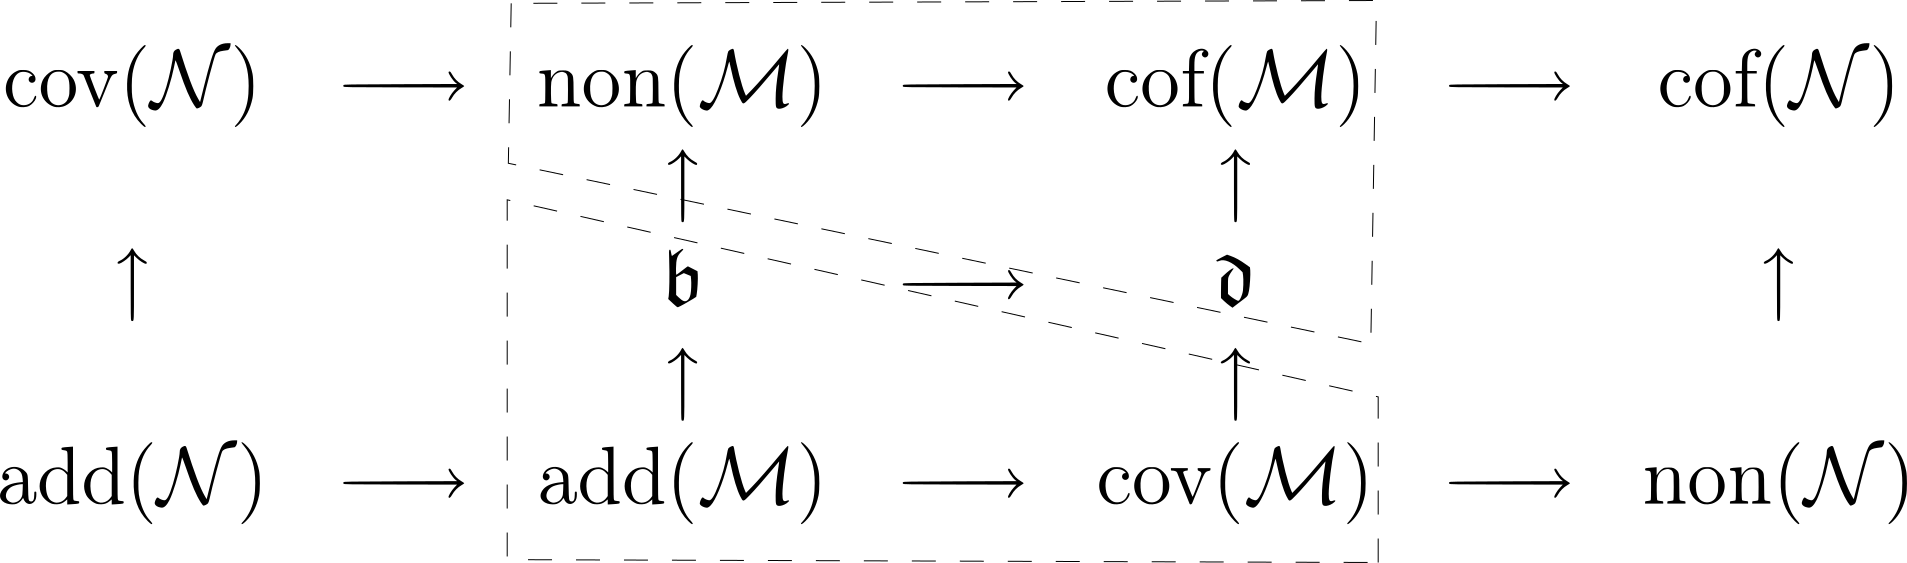
\includegraphics[height=3cm]{work_in_progress/cichon-2.pdf}
\end{center}

It is a direct consequence of the following reformulation of the cardinal invariants in terms of norms of triples:

\begin{theorem}
 \begin{displaymath}
\begin{array}{ccccccc}

(\R,\N,\in)        &\longrightarrow & (\M,\R,\not\ni)                         &\longrightarrow & (\M,\M,\subset)                    & \longrightarrow &(\N,\N,\subset)\cr
                   &                & \uparrow                                &                &\uparrow                            &                 &               \cr
\uparrow           &                & (\omega^\omega,\omega^\omega,\not\geq^*)&\longrightarrow &(\omega^\omega,\omega^\omega,\leq^*)&                 &\uparrow       \cr
                   &                & \uparrow                                &                &\uparrow                            &                 &               \cr
(\N,\N,\not\supset)&\longrightarrow & (\M,\M,\not\supset)                     &\longrightarrow &(\R,\M,\in)                         & \longrightarrow &(\N,\R,\not\ni)\cr
\end{array}
\end{displaymath}
\end{theorem}

A summary of the connections between different cardinal invariants can be seen in the following diagram. It is a fusion of
Cicho\'n's diagram with van Douwen's diagram which can be found in \cite{Bl:2009} (see also \cite{Br:2006}):

\begin{center}
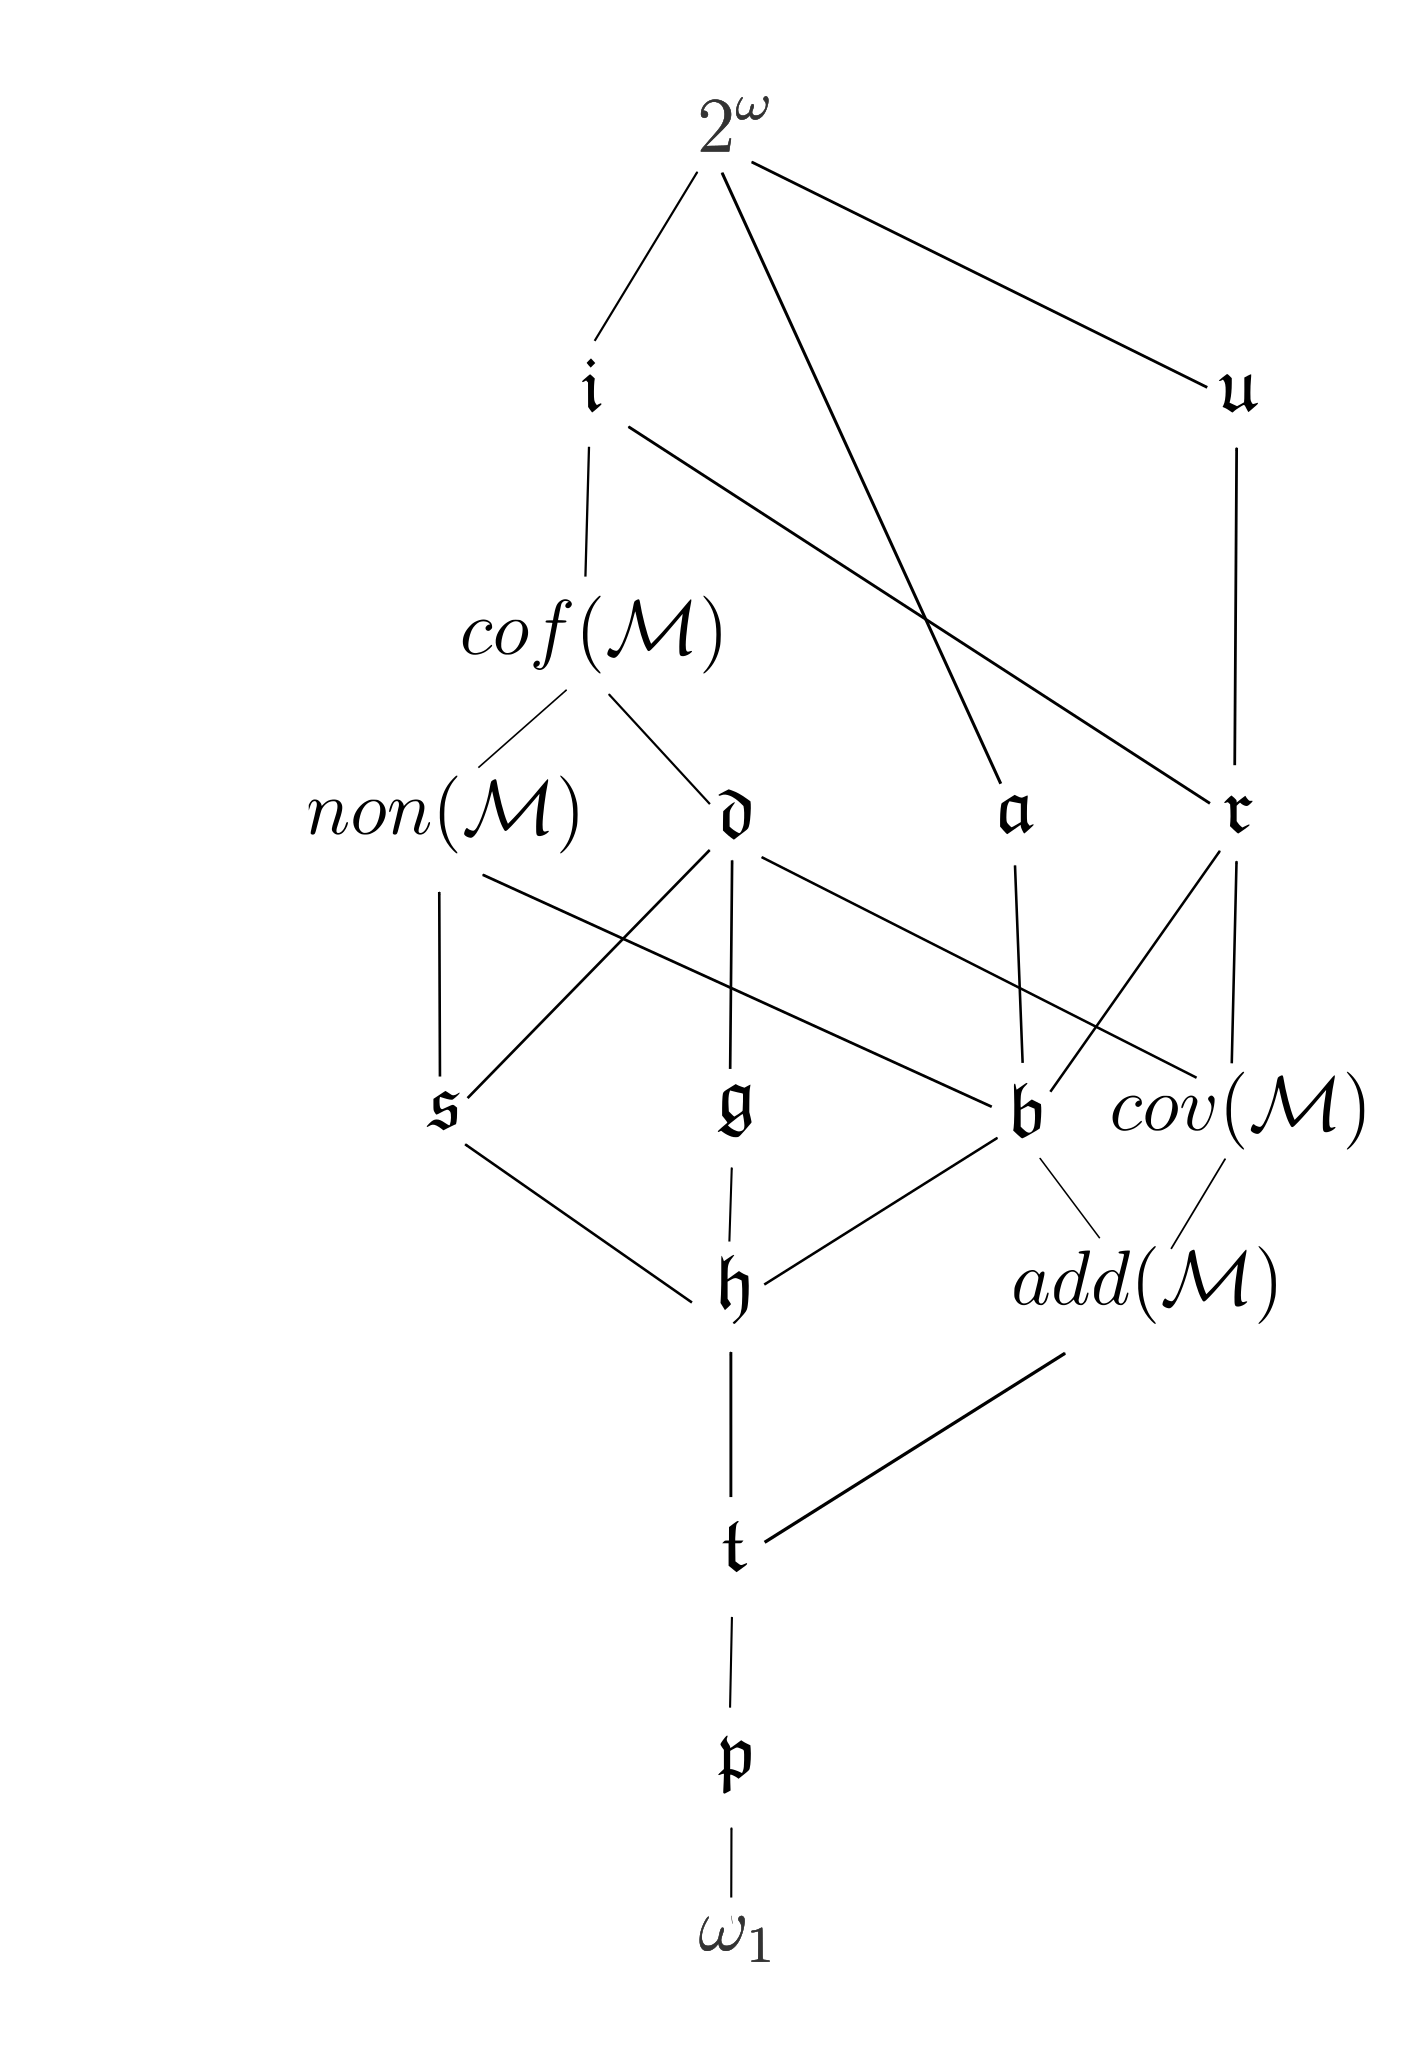
\includegraphics[height=10cm]{work_in_progress/cardinal-invariants-diagram-varIII.pdf}
\end{center}

The dashed boxes indicate, respectively, that the top cardinal and bottom cardinal are the maximum and the minimum of the other
two cardinals.
\subsection{iteration}

% \subsubsection{Martin's axiom}
%
% Take $\kappa$ s.t., $\kappa^{<\kappa}=\kappa$. Consider $\mathcal S=\{(P,\leq):P\subseteq \kappa, |P|<\kappa\}$ ordered by regular embedding.
% If $B$ is a generic on $S$ then forcing with $B$ gives us MA.


\subsubsection{Preservation theorems}
\begin{definition} An ordering $P$ is \emph{$n$-linked}, $n<\omega$, if for any $X\in[P]^{\leq n}$ there is
$p\in P$ compatible with each $x\in X$. \emph{Linked} is short for $2$-linked. An ordering has the \emph{Knaster} property if any uncountable subset of the ordering contains an uncountable linked subset.
\end{definition}

\begin{obs} If $P$ has the Knaster property then given $n<\omega$ any uncountable subset contains
 an uncountable $n$-linked subset.
\end{obs}
\begin{proof} Easy, inductively apply the Knaster property to the witnesses for $2$-linkedness.
\end{proof}

\begin{proposition} If $P$ is an ordering with the Knaster property and $P\force\dot{Q}$ has the Knaster
 property then $P*\dot{Q}$ has the Knaster property.
\end{proposition}
\begin{proof}
 Let $\{\langle p_\alpha,\dot{q}_\alpha\rangle:\alpha<\omega_1\}\subseteq P*\dot{Q}$.
 By strengthening the $p_\alpha$'s we may assume that each $p_\alpha$ decides the statement

 \begin{displaymath}
  \{\dot{q}_\alpha:\alpha< \omega_1\}\ \hbox{is uncountable}
 \end{displaymath}

 By the above observation we may assume that the $p_\alpha$'s are $4$-linked. We also assume that all the
 $p_\alpha$'s decide the statement in the same way. There are two cases:

 {\bf Case 1.} Each $p_\alpha$ forces that $\{\dot{q}_\alpha:\alpha<\omega_1\}$ is uncountable. Working
 in $RO(P)$ (which also has the Knaster property) let $b=\bigvee\{p_\alpha\}$. Then $b$ forces that
 $\{\dot{q}_\alpha:\alpha<\omega_1\}$ is uncountable and since $P\force\dot{Q}$ has the Knaster property,
 there is a name $\dot{X}$ such that
 \begin{displaymath}
  b\force \dot{X}\subseteq\{\dot{q}_\alpha:\alpha<\omega_1\}\ \&\ |\dot{X}|=\omega_1\ \&\ \dot{X}\
  \mbox{is linked}.
 \end{displaymath}
 By induction to $\omega_1$ choose
 $\{\langle r_\alpha,\dot{s}_\alpha\rangle :\alpha<\omega_1\}\subseteq
  \{\langle p_\beta,\dot{q}_\beta\rangle:\beta<\omega\}$
 such that $r_\alpha\force \dot{s}_{\alpha+1}\in\dot{X}$. This is possible since each $p_\alpha$
 forces $\dot{X}$ to be uncountable. We claim that
 $\{\langle r_{\alpha+1},\dot{s}_{\alpha+1}\rangle:\alpha<\omega_1\}$
 is linked. Choose $\alpha,\beta<\omega_1$. Since we assumed the $p_\alpha$'s are $4$-linked we may find
 $p\in P$ be below $r_\alpha,r_{\alpha+1},r_\beta,r_{\beta+1}$.
 Then $p\force \dot{s}_{\alpha+1},\dot{s}_{\beta+1}\in \dot{X}$ so $p$ knows they are compatible so there
 is $\dot{t}\in \dot{Q}$ such that $p\force \dot{t}\leq \dot{s}_{\alpha+1},\dot{s}_{\beta+1}$. Then
 $\langle p,\dot{t}\rangle\leq\langle r_{\alpha+1},\dot{s}_{\alpha+1}\rangle,\langle r_{\beta+1},dot{s}_{\beta+1}\rangle$ and this finishes the proof of case 1.

 {\bf Case 2.} There is $R=\{\dot{r}_n:n<\omega\}\subseteq\dot{Q}$ such that
 $\dot{p}_\alpha\force\dot{q}_\alpha\in R$. Again work in $RO(P)$ and find, below each $p_\alpha$
 an antichain $b_{\alpha,n}$ such that $b_{\alpha,n}=||\dot{q}_\alpha=\dot{r}_n||$.
 By the Knaster property for $RO(P)$ there is an uncountable set $I\subseteq\omega_1\times\omega$
 such that for each $(\alpha,n),(\beta,m)\in I$ the corresponding $b_{\alpha,n}$ and $b_{\beta,m}$
 are compatible. Since $I$ is uncountable we may assume that the second coordinates are all equal to
 some $n_0<\omega$ and then $b_{\alpha,n_0}\leq p_\alpha$ and $b_{\alpha,n_0}\force \dot{q}_\alpha=\dot{r}_n$
 so they witness that $\langle p_\alpha,\dot{q}_\alpha\rangle$ are pairwise compatible.

\end{proof}


%%%%%%%%%%%%%%%%%%%%%%%%%%%%%%%%%%%%%%%%%%%%%%%%%%%%%%%%%%%%%%%%%%%%%%%
%%%                          END                                    %%%
%%%%%%%%%%%%%%%%%%%%%%%%%%%%%%%%%%%%%%%%%%%%%%%%%%%%%%%%%%%%%%%%%%%%%%%

%-------------------------------------------------------------
%-------------------------------------------------------------
%-------------------------------------------------------------
%-------------------------------------------------------------
\nocite{ArTo:05}\nocite{BaSt}\nocite{BaJu:95}\nocite{Ke:1994}\nocite{Handbook1}\nocite{KunST}
\nocite{Sh:98}\nocite{Zap:08}\nocite{BlTu}\nocite{goldstern}\nocite{kanamori}\nocite*
% \nocite{}\nocite{}\nocite{}\nocite{}\nocite{}\nocite{}
% \nocite{}\nocite{}\nocite{}\nocite{}\nocite{}\nocite{}\nocite{}\nocite{}
% \nocite{}\nocite{}\nocite{}\nocite{}\nocite{}\nocite{}\nocite{}\nocite{}
% \nocite{}\nocite{}\nocite{}\nocite{}\nocite{}\nocite{}\nocite{}\nocite{}

%--------------------REFERENCES------------------------------
\bibliographystyle{alpha}\addcontentsline{toc}{chapter}{References}
\lhead{{\scshape References}}
\bibliography{entree}


%...................l_entree.ind....................................
%\include{index}

%..............................................................


\end{document}
